%%-----------------------------------------------------------------------------
%%
%%                                   Sean Mauch
%%                       California Institute of Technology
%%                          (a) 2000 No Rights Reserved
%%
%%-----------------------------------------------------------------------------

%% CONTINUE Consider integrating \frac{1}{\sin(\pi/z)} on the circle of
%% radius 2 as an application of the residue at infinity







%%============================================================================
%%============================================================================
\flushbottom
\chapter{The Residue Theorem}





Man will occasionally stumble over the truth, but most of the time 
he will pick himself up and continue on.

\begin{flushright}
  - Winston Churchill
\end{flushright}











%%=============================================================================
\section{The Residue Theorem}




We will find that many integrals on closed contours may be evaluated
in terms of the \textit{residues} of a function.  We first define
residues and then prove the Residue Theorem.


\begin{Result}
  \index{residues}
  \index{Laurent expansions}
  \index{residues!of a pole of order $n$}
  \textbf{Residues.}
  Let $f(z)$ be single-valued an analytic in a deleted neighborhood of $z_0$.
  Then $f(z)$ has the Laurent series expansion
  \[ 
  f(z) = \sum_{n=-\infty}^{\infty} a_n (z-z_0)^n, 
  \]
  The residue of $f(z)$ at $z = z_0$ is the coefficient of the $\frac{1}{z-z_0}$
  term:
  \[ 
  \Res(f(z),z_0) = a_{-1}.
  \]
  The residue at a branch point or non-isolated singularity is undefined as 
  the Laurent series does not exist.
  If $f(z)$ has a pole of order $n$ at $z=z_0$ then we can use the 
  Residue Formula:
  \[
  \Res(f(z),z_0) = \lim_{z \to z_0} \left( \frac{1}{(n-1)!}
    \frac{\dd^{n-1}}{\dd z^{n-1}}\big[(z-z_0)^n f(z)\big] \right). 
  \]
\end{Result}

See Exercise~\ref{exercise residue formula} for a proof of the Residue Formula.




\begin{Example}
  In Example~\ref{example_z_sin_z} we showed that $f(z) = z/\sin z$ 
  has first order poles at $z = n \pi$, $n \in \mathbb{Z} \setminus \{ 0 \}$.
  Now we find the residues at these isolated singularities.
  \begin{align*}
    \Res \left( \frac{z}{\sin z}, z = n \pi \right)
    &= \lim_{z \to n\pi} \left( \left( z-n\pi \right) 
      \frac{z}{\sin z} \right) \\
    &= n\pi \lim_{z \to n\pi} \frac{z-n\pi}{\sin z} \\
    &= n\pi \lim_{z \to n \pi} \frac{1}{\cos z} \\
    &= n\pi \frac{1}{(-1)^n} \\
    &= (-1)^n n \pi
  \end{align*}
\end{Example}






\paragraph{Residue Theorem.}
We can evaluate many integrals in terms of the residues of a function.
Suppose $f(z)$ has only one singularity, (at $z = z_0$), inside the 
simple, closed, positively oriented contour $C$.  $f(z)$ has a convergent 
Laurent series in some deleted disk about $z_0$.  We deform $C$ to lie in 
the disk.  See Figure~\ref{deformc2b}.  We now evaluate $\int_C f(z) \,\dd z$
by deforming the contour and using the Laurent series expansion of the 
function.

\begin{figure}[tb!]
  \begin{center}
    
\includegraphics[width=0.4\textwidth]{fcv/residue/deformc2b}
  \end{center}
  \caption{Deform the contour to lie in the deleted disk.}
  \label{deformc2b}
\end{figure}

\begin{align*}
  \int_C f(z) \,\dd z
  &= \int_B f(z) \,\dd z \\
  &= \int_B \sum_{n = - \infty}^\infty a_n (z - z_0)^n \,\dd z \\
  &= \sum_{\substack{n = - \infty \\ n \neq -1}}^\infty a_n \left[ \frac{ (z - z_0)^{n+1} }{ n+1 } 
  \right]_{r \e^{\imath \theta}}^{r \e^{\imath (\theta + 2 \pi)}}
  + a_{-1} \left[ \log(z - z_0) \right]_{r \e^{\imath \theta}}^{r \e^{\imath (\theta + 2 \pi)}} \\
  &= a_{-1} \imath 2 \pi
\end{align*}
\[
\int_C f(z) \,\dd z = \imath 2 \pi \Res( f(z), z_0 )
\]


Now assume that $f(z)$ has $n$ singularities at $\{ z_1, \ldots, z_n \}$.
We deform $C$ to $n$ contours $C_1, \ldots, C_n$ which enclose the singularities
and lie in deleted disks about the singularities in which $f(z)$ has 
convergent Laurent series.  See Figure~\ref{deformc2cn}.  We evaluate
$\int_C f(z) \,\dd z$ by deforming the contour.
\[
\int_C f(z) \,\dd z 
= \sum_{k = 1}^n \int_{C_k} f(z) \,\dd z
= \imath 2 \pi \sum_{k = 1}^n \Res( f(z), z_k )
\]


\begin{figure}[tb!]
  \begin{center}
    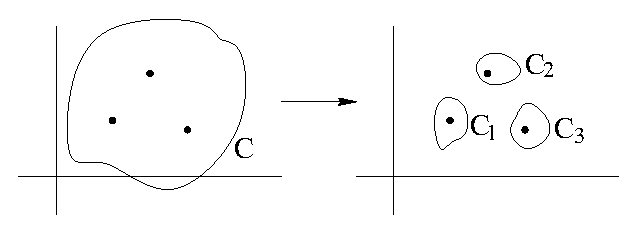
\includegraphics[width=0.4\textwidth]{fcv/residue/deformc2cn}
  \end{center}
  \caption{Deform the contours which enclose the singularities.}
  \label{deformc2cn}
\end{figure}



Now instead let $f(z)$ be analytic \textit{outside} and on $C$ 
except for isolated singularities at $\{ \zeta_n \}$ in the domain outside $C$ and
perhaps an isolated singularity at infinity.
Let $a$ be any point in the interior of $C$.
To evaluate $\int_C f(z) \,\dd z$ we make the change of variables
$\zeta = 1 / (z-a)$.  This maps the contour $C$ to $C'$.  (Note that $C'$ is
negatively oriented.)  All the points outside
$C$ are mapped to points inside $C'$ and vice versa.  We can then evaluate
the integral in terms of the singularities inside $C'$.

\begin{align*}
  \oint_C f(z)\,\dd z 
  &= \oint_{C'} f \left( \frac{1}{\zeta} + a \right) \frac{-1}{\zeta^2} \,\dd \zeta \\
  &= \oint_{-C'} \frac{1}{z^2} f \left(\frac{1}{z} + a \right) \,\dd z \\
  &= \imath 2 \pi \sum_n \Res \left( \frac{1}{z^2} f \left(\frac{1}{z} + a \right), 
    \frac{1}{\zeta_n - a} \right)
  + \imath 2 \pi \Res \left( \frac{1}{z^2} f \left(\frac{1}{z} + a \right), 0 \right).
\end{align*}


\begin{figure}[tb!]
  \begin{center}
    \includegraphics[width=0.5\textwidth]{fcv/residue/changevarz1za}
  \end{center}
  \caption{The change of variables.}
  \label{changevarz1za}
\end{figure}



\begin{Result}
  \index{residue theorem}
  \textbf{Residue Theorem.}
  If $f(z)$ is analytic in a compact, closed, connected domain $D$
  except for isolated singularities at $\{ z_n \}$ in the interior of $D$ then
  \[ 
  \int_{\partial D} f(z)\,\dd z 
  = \sum_k \oint_{C_k} f(z)\,\dd z 
  = \imath 2 \pi \sum_n \Res(f(z),z_n).
  \]
  Here the set of contours $\{ C_k \}$ make up the positively oriented boundary
  $\partial D$ of the domain $D$.  If the boundary of the domain is a single contour 
  $C$ then the formula simplifies.
  \[ 
  \oint_C f(z)\,\dd z = \imath 2 \pi \sum_n \Res(f(z),z_n)
  \]
  If instead $f(z)$ is analytic outside and on $C$ 
  except for isolated singularities at $\{ \zeta_n \}$ in the domain outside $C$ and
  perhaps an isolated singularity at infinity then
  \[ 
  \oint_C f(z)\,\dd z 
  = \imath 2 \pi \sum_n \Res \left( \frac{1}{z^2} f \left(\frac{1}{z} + a \right), 
    \frac{1}{\zeta_n - a} \right)
  + \imath 2 \pi \Res \left( \frac{1}{z^2} f \left(\frac{1}{z} + a \right), 0 \right).
  \]
  Here $a$ is a any point in the interior of $C$.
\end{Result}








\begin{Example}
  Consider
  \[
  \frac{1}{\imath 2 \pi}\int_C \frac{\sin z}{z(z-1)} \,\dd z
  \]
  where $C$ is the positively oriented circle of radius 2 centered at the origin.
  Since the integrand is single-valued with only isolated singularities, 
  the Residue Theorem applies.  The value of the integral is the sum of 
  the residues from singularities inside the contour.

  The only places that the integrand could have singularities are $z = 0$ and
  $z = 1$.  Since
  \[
  \lim_{z \to 0} \frac{\sin z}{z} = \lim_{z \to 0} \frac{\cos z}{1} = 1,
  \]
  there is a removable singularity at the point $z = 0$.  There is no residue
  at this point.

  Now we consider the point $z = 1$.
  Since $\sin(z) / z$ is analytic and nonzero at $z = 1$, that point is a 
  first order pole of the integrand.  The residue there is
  \[
  \Res \left( \frac{ \sin z }{ z (z-1) }, z = 1 \right)
  = \lim_{z \to 1} (z - 1) \frac{ \sin z }{ z (z-1) }
  = \sin(1).
  \]

  There is only one singular point with a residue inside the path of integration.
  The residue at this point is $\sin(1)$.  Thus the value of the integral is
  \[
  \frac{1}{\imath 2 \pi}\int_C \frac{\sin z}{z(z-1)} \,\dd z = \sin(1)
  \]
\end{Example}





















\begin{Example}
  Evaluate the integral
  \[
  \int_C \frac{\cot z  \coth z}{z^3} \,\dd z
  \]
  where $C$ is the unit circle about the origin in the positive direction.

  The integrand is
  \[
  \frac{\cot z  \coth z}{z^3} = \frac{\cos z \cosh z}{z^3 \sin z  \sinh z}
  \]
  $\sin z$ has zeros at $n\pi$.  $\sinh z$ has zeros at $\imath n \pi$.  Thus
  the only pole inside the contour of integration is at $z = 0$.
  Since $\sin z$ and $\sinh z$ both have simple zeros at $z=0$,
  \[
  \sin z = z + \mathcal{O}(z^3), \qquad \sinh z = z + \mathcal{O}(z^3)
  \]
  the integrand has a pole of order 5 at the origin.
  The residue at $z=0$ is
  \begin{align*}
    \lim_{z \to 0} \frac{1}{4!} \frac{\dd^4}{\dd z^4} \left( z^5
      \frac{\cot z  \coth z}{z^3} \right)
    &= \lim_{z \to 0} \frac{1}{4!} \frac{\dd^4}{\dd z^4} \left( z^2
      \cot z  \coth z \right) \\
    &= \frac{1}{4!} \lim_{z \to 0} \bigg(
    24 \cot (z) \coth (z) {{\csc (z)}^2} -
    32 z \coth (z) {{\csc (z)}^4}  \\
    &\qquad -
    16 z \cos (2 z) \coth (z) {{\csc (z)}^4} +
    22 {z^2} \cot (z) \coth (z) {{\csc (z)}^4}  \\
    &\qquad +
    2 {z^2} \cos (3 z) \coth (z) {{\csc (z)}^5} +
    24 \cot (z) \coth (z) {{{\csch}(z)}^2} \\
    &\qquad +
    24 {{\csc (z)}^2} {{{\csch}(z)}^2} -
    48 z \cot (z) {{\csc (z)}^2} {{{\csch}(z)}^2}  \\
    &\qquad -
    48 z \coth (z) {{\csc (z)}^2} {{{\csch}(z)}^2} +
    24 {z^2} \cot (z) \coth (z) {{\csc (z)}^2}
    {{{\csch}(z)}^2} \\
    &\qquad + 16 {z^2} {{\csc (z)}^4}
    {{{\csch}(z)}^2} + 8 {z^2} \cos (2 z)
    {{\csc (z)}^4} {{{\csch}(z)}^2}  \\
    &\qquad -
    32 z \cot (z) {{{\csch}(z)}^4} -
    16 z \cosh (2 z) \cot (z) {{{\csch}(z)}^4}  \\
    &\qquad +
    22 {z^2} \cot (z) \coth (z) {{{\csch}(z)}^4} +
    16 {z^2} {{\csc (z)}^2} {{{\csch}(z)}^4} \\
    &\qquad +
    8 {z^2} \cosh (2 z) {{\csc (z)}^2}
    {{{\csch}(z)}^4} + 2 {z^2} \cosh (3 z) \cot (z)
    {{{\csch}(z)}^5} \bigg) \\
    &= \frac{1}{4!} \left( -\frac{56}{15} \right) \\
    &= -\frac{7}{45}
  \end{align*}

  Since taking the fourth derivative of $z^2 \cot z  \coth z$ really sucks, we
  would like a more elegant way of finding the residue.  We expand the
  functions in the integrand in Taylor series about the origin.
  \begin{align*}
    \frac{\cos z \cosh z}{z^3 \sin z  \sinh z}
    &= \frac{\left( 1 - \frac{z^2}{2} + \frac{z^4}{24} - \cdots \right)
      \left(1 + \frac{z^2}{2} + \frac{z^4}{24} + \cdots \right)}{z^3
      \left(z - \frac{z^3}{6} + \frac{z^5}{120} - \cdots \right)
      \left(z + \frac{z^3}{6} + \frac{z^5}{120} + \cdots \right)} \\
    &= \frac{1 - \frac{z^4}{6} + \cdots }
    {z^3 \left(z^2 + z^6 \left( \frac{-1}{36} + \frac{1}{60}
        \right)  + \cdots \right) } \\
    &= \frac{1}{z^5} \frac{1 - \frac{z^4}{6} + \cdots }
    {1 - \frac{z^4}{90} + \cdots } \\
    &= \frac{1}{z^5} \left( 1 - \frac{z^4}{6} + \cdots  \right)
    \left( 1 + \frac{z^4}{90} + \cdots  \right) \\
    &= \frac{1}{z^5} \left(1 - \frac{7}{45} z^4 + \cdots \right) \\
    &= \frac{1}{z^5} -\frac{7}{45} \frac{1}{z} + \cdots
  \end{align*}
  Thus we see that the residue is $-\frac{7}{45}$.
  Now we can evaluate the integral.
  \[
  \int_C \frac{\cot z  \coth z}{z^3} \,\dd z = - \imath \frac{14}{45} \pi
  \]
\end{Example}










%% CONTINUE
%% Consider integrating over a pole at infinity.






%%=============================================================================
\section{Cauchy Principal Value for Real Integrals}











%%-----------------------------------------------------------------------------
\subsection{The Cauchy Principal Value}
\index{principal value}
\index{Cauchy principal value}



First we recap improper integrals.  If $f(x)$ has a singularity at
$x_0 \in (a \ldots b)$ then
\[
\int_a^b f(x) \,\dd x \equiv \lim_{\epsilon \to 0^+} \int_a^{x_0 - \epsilon} f(x) \,\dd x
+ \lim_{\delta \to 0^+} \int_{x_0 + \delta}^b f(x) \,\dd x.
\]
For integrals on $(-\infty \ldots \infty)$,
\[
\int_{-\infty}^\infty f(x) \,\dd x \equiv \lim_{a \to -\infty,\ b \to \infty} \int_a^b f(x) \,\dd x.
\]




\begin{Example}
  $\int_{-1}^1 \frac{1}{x} \,\dd x$ is divergent.  We show this with the definition 
  of improper integrals.
  \begin{align*}
    \int_{-1}^1 \frac{1}{x} \,\dd x
    &= \lim_{\epsilon \to 0^+} \int_{-1}^{-\epsilon} \frac{1}{x} \,\dd x
    + \lim_{\delta \to 0^+} \int_{\delta}^1 \frac{1}{x} \,\dd x \\
    &= \lim_{\epsilon \to 0^+} \left[ \ln|x| \right]_{-1}^{-\epsilon}
    + \lim_{\delta \to 0^+} \left[ \ln|x| \right]_\delta^1 \\
    &= \lim_{\epsilon \to 0^+} \ln \epsilon
    - \lim_{\delta \to 0^+} \ln \delta
  \end{align*}
  The integral diverges because $\epsilon$ and $\delta$ approach zero independently.

  Since $1 / x$ is an odd function, it appears that the area under the
  curve is zero.  Consider what would happen if $\epsilon$ and $\delta$ were not
  independent.  If they approached zero symmetrically, $\delta = \epsilon$, then
  the value of the integral would be zero.
  \[
  \lim_{\epsilon \to 0^+} \left( \int_{-1}^{-\epsilon} + \int_\epsilon^1 \right) \frac{1}{x} \,\dd x
  = \lim_{\epsilon \to 0^+} ( \ln \epsilon - \ln \epsilon ) = 0
  \]
  We could make the integral have any value we pleased by choosing $\delta = c \epsilon$.
  \footnote{This may remind you of conditionally convergent series.  You can 
    rearrange the terms to make the series sum to any number.}
  %% CONTINUE reference exercise.
  \[
  \lim_{\epsilon \to 0^+} \left( \int_{-1}^{-\epsilon} + \int_{c \epsilon}^1 \right) \frac{1}{x} \,\dd x
  = \lim_{\epsilon \to 0^+} ( \ln \epsilon - \ln(c \epsilon) ) = - \ln c
  \]
\end{Example}





We have seen it is reasonable that 
\[
\int_{-1}^1 \frac{1}{x} \,\dd x
\]
has some meaning, and if we could evaluate the integral, the most 
reasonable value would be zero.  The \textit{Cauchy principal value} 
provides us with a way of evaluating such integrals.
If $f(x)$ is continuous on $(a,b)$ except at the point $x_0 \in (a,b)$ then 
the Cauchy principal value of the integral is defined
\[
\pv \int_a^b f(x) \,\dd x = \lim_{\epsilon \to 0^+} \left(
  \int_a^{x_0-\epsilon} f(x) \,\dd x
  + \int_{x_0+\epsilon}^b f(x) \,\dd x \right).
\]
The Cauchy principal value is obtained by approaching the singularity 
symmetrically.
The principal value of the integral may exist when the integral diverges.
If the integral exists, it is equal to the principal value of the integral.

The Cauchy principal value of $\int_{-1}^1 \frac{1}{x} \,\dd x$ is defined
\begin{align*}
  \pv \int_{-1}^1 \frac{1}{x} \,\dd x 
  &\equiv \lim_{\epsilon \to 0^+} \left( \int_{-1}^{-\epsilon} 
    \frac{1}{x} \,\dd x + \int_\epsilon^1 \frac{1}{x} \,\dd x \right) \\
  &= \lim_{\epsilon \to 0^+} \left( 
    \left[ \log |x| \right]_{-1}^{-\epsilon}
    \left[ \log |x| \right]_\epsilon^1 \right) \\
  &= \lim_{\epsilon \to 0^+} \left( \log |-\epsilon| -
    \log | \epsilon | \right) \\
  &= 0.
\end{align*}
(Another notation for the principal value of an integral is
$\PV \int f(x)\,\dd x$.)
Since the limits of integration approach zero symmetrically, the two halves
of the integral cancel.  If the limits of integration approached
zero independently, (the definition of the integral), then the two halves
would  both diverge.






\begin{Example}
  $\int_{-\infty}^\infty \frac{x}{x^2 + 1} \,\dd x$ is divergent.  
  We show this with the definition of improper integrals.
  \begin{align*}
    \int_{-\infty}^\infty \frac{x}{x^2 + 1} \,\dd x
    &= \lim_{a \to -\infty,\ b \to \infty} \int_a^b \frac{x}{x^2 + 1} \,\dd x \\
    &= \lim_{a \to -\infty,\ b \to \infty} \left[ \frac{1}{2} \ln(x^2+1) \right]_a^b \\
    &= \frac{1}{2} \lim_{a \to -\infty,\ b \to \infty} \ln \left( \frac{b^2+1}{a^2+1} \right)
  \end{align*}
  The integral diverges because $a$ and $b$ approach infinity independently.
  Now consider what would happen if $a$ and $b$ were not independent.
  If they approached zero symmetrically, $a = -b$, then the value 
  of the integral would be zero.
  \[
  \frac{1}{2} \lim_{b \to \infty} \ln \left( \frac{b^2+1}{b^2+1} \right) = 0
  \]
  We could make the integral have any value we pleased by choosing $a = - c b$.
\end{Example}



We can assign a meaning to divergent integrals of the form
$\int_{-\infty}^\infty f(x) \,\dd x$ with the Cauchy principal value.
The Cauchy principal value of the integral is defined
\[
\pv \int_{-\infty}^\infty f(x) \,\dd x = \lim_{a \to \infty} \int_{-a}^a f(x) \,\dd x.
\]
The Cauchy principal value is obtained by approaching infinity
symmetrically.

The Cauchy principal value of $\int_{-\infty}^\infty \frac{x}{x^2+1} \,\dd x$ is defined
\begin{align*}
  \pv \int_{-\infty}^\infty \frac{x}{x^2+1} \,\dd x 
  &= \lim_{a \to \infty} \int_{-a}^a \frac{x}{x^2+1} \,\dd x \\
  &= \lim_{a \to \infty} \left[ \frac{1}{2} \ln \left( x^2+1 \right) \right]_{-a}^a \\
  &= 0.
\end{align*}




\begin{Result}
  \textbf{Cauchy Principal Value.}
  If $f(x)$ is continuous on $(a,b)$ except at the point $x_0 \in (a,b)$ then 
  the integral of $f(x)$ is defined
  \[
  \int_a^b f(x) \,\dd x = \lim_{\epsilon \to 0^+} \int_a^{x_0-\epsilon} f(x) \,\dd x
  + \lim_{\delta \to 0^+} \int_{x_0+\delta}^b f(x) \,\dd x.
  \]
  The Cauchy principal value of the integral is defined
  \[
  \pv \int_a^b f(x) \,\dd x = \lim_{\epsilon \to 0^+} \left(
    \int_a^{x_0-\epsilon} f(x) \,\dd x
    + \int_{x_0+\epsilon}^b f(x) \,\dd x \right).
  \]

  If $f(x)$ is continuous on $(-\infty,\infty)$ then the integral of $f(x)$ is defined
  \[
  \int_{-\infty}^\infty f(x) \,\dd x = \lim_{a \to -\infty,\ b \to \infty} \int_a^b f(x) \,\dd x.
  \]
  The Cauchy principal value of the integral is defined
  \[
  \pv \int_{-\infty}^\infty f(x) \,\dd x = \lim_{a \to \infty} \int_{-a}^a f(x) \,\dd x.
  \]

  The principal value of the integral may exist when the integral diverges.
  If the integral exists, it is equal to the principal value of the integral.
\end{Result}




\begin{Example}
  Clearly $\int_{-\infty}^\infty x \,\dd x$ diverges, however the Cauchy principal value exists.
  \[
  \pv \int_{-\infty}^\infty x \,\dd x 
  = \lim_{a \to \infty} \left[ \frac{x^2}{2} \right]_{-a}{a} 
  = 0
  \]
  In general, if $f(x)$ is an odd function with no singularities on the finite 
  real axis then
  \[
  \pv \int_{-\infty}^\infty f(x) \,\dd x = 0.
  \]
\end{Example}









%%=============================================================================
\section{Cauchy Principal Value for Contour Integrals}





\begin{Example}
  Consider the integral
  \[
  \int_{C_r} \frac{1}{z-1} \,\dd z,
  \]
  where $C_r$ is the positively oriented circle of radius $r$ and center at 
  the origin.  From the residue theorem, we know that the integral is
  \[
  \int_{C_r} \frac{1}{z-1} \,\dd z
  = \begin{cases}
    0 \quad &\mathrm{for}\ r < 1, \\
    \imath 2 \pi \quad &\mathrm{for}\ r > 1.
  \end{cases}
  \]
  When $r=1$, the integral diverges, as there is a first order pole on the
  path of integration.  However, the principal value of the integral exists.
  \begin{align*}
    \pv \int_{C_r} \frac{1}{z-1} \,\dd z
    &= \lim_{\epsilon \to 0^+} \int_\epsilon^{2\pi - \epsilon}
    \frac{1}{e^{\imath \theta} - 1} \imath e^{\imath \theta} \,\dd \theta \\
    &= \lim_{\epsilon \to 0^+} \left[ \log(e^{\imath \theta}-1)
    \right]_\epsilon^{2\pi - \epsilon} \\
    \intertext{We choose the branch of the logarithm with a branch cut on the 
      positive real axis and $\arg\log z \in (0,2\pi)$.}
    &= \lim_{\epsilon \to 0^+} \left( 
      \log \left( e^{\imath (2\pi - \epsilon)} - 1  \right) -
      \log \left( e^{\imath \epsilon} - 1 \right) \right) \\
    &= \lim_{\epsilon \to 0^+} \left( 
      \log \left( \left( 1 - i\epsilon + O(\epsilon^2) \right) - 1 \right) -
      \log \left( \left( 1 + i\epsilon + O(\epsilon^2) \right) - 1 \right) 
    \right) \\
    &= \lim_{\epsilon \to 0^+} \left( 
      \log \left( - i\epsilon + O(\epsilon^2) \right) -
      \log \left( i\epsilon + O(\epsilon^2) \right) 
    \right) \\
    &= \lim_{\epsilon \to 0^+} \left( 
      \Log \left( \epsilon + O(\epsilon^2) \right) 
      + \imath \arg\left( -\imath \epsilon + O(\epsilon^2) \right) -
      \Log \left( \epsilon + O(\epsilon^2) \right) 
      - \imath \arg\left( \imath \epsilon + O(\epsilon^2) \right)
    \right) \\
    &= \imath \frac{3\pi}{2} - \imath \frac{\pi}{2} \\
    &= \imath \pi
  \end{align*}
  Thus we obtain 
  \[
  \boxed{
    \pv \int_{C_r} \frac{1}{z-1} \,\dd z
    = \begin{cases}
      0 \quad &\mathrm{for}\ r < 1, \\
      \imath \pi \quad &\mathrm{for}\ r = 1, \\
      \imath 2 \pi \quad &\mathrm{for}\ r > 1.
    \end{cases}
    }
  \]
\end{Example}



In the above example we evaluated the contour integral by parameterizing
the contour.  This approach is only feasible when the integrand is
simple.  We would like to use the residue theorem to more easily
evaluate the principal value of the integral.  But before we do
that, we will need a preliminary result.





\begin{Result}
  \label{cpv_arcint}
  Let $f(z)$ have a first order pole at $z=z_0$ and let $(z-z_0)f(z)$ be 
  analytic in some neighborhood of $z_0$.  Let the contour $C_\epsilon$
  be a circular arc from $z_0 + \epsilon e^{\imath \alpha}$ to 
  $z_0 + \epsilon e^{\imath \beta}$.  (We assume that $\beta > \alpha$ and 
  $\beta - \alpha < 2\pi$.)
  \[
  \lim_{\epsilon \to 0^+} \int_{C_\epsilon} f(z) \,\dd z =
  \imath (\beta - \alpha) \Res( f(z), z_0 )
  \]
  The contour is shown in Figure~\ref{cpv_ceab}.
  (See Exercise~\ref{exercise int ce f(z)} for a proof of this result.)
\end{Result}



\begin{figure}[tb!]
  \begin{center}
    \includegraphics[width=0.2\textwidth]{fcv/residue/cpv_ceab}
  \end{center}
  \caption{The contour.}
  \label{cpv_ceab}
\end{figure}









\begin{Example}
  \label{cpv_exind}
  Consider 
  \[
  \pv \int_C \frac{1}{z-1} \,\dd z
  \]
  where $C$ is the unit circle.
  Let $C_p$ be the circular arc of radius 1 that starts and ends a distance
  of $\epsilon$ from $z=1$.  Let $C_\epsilon$ be the positive,
  circular arc of radius $\epsilon$ with center at $z=1$ that joins the endpoints
  of $C_p$.  Let $C_i$, be the union of $C_p$ and $C_\epsilon$.  ($C_p$ stands
  for Principal value Contour; $C_i$ stands for Indented Contour.)  $C_i$ is
  an indented contour that avoids the first order pole at $z=1$.  
  Figure~\ref{cpv_cpce} shows the three contours.

  %% CONTINUE Make into 3 graphs: C_i, C_p and C_\epsilon.
  \begin{figure}[tb!]
    \begin{center}
      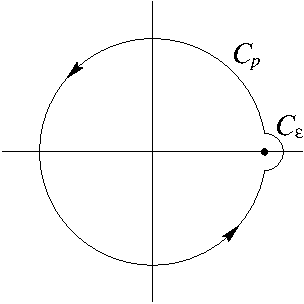
\includegraphics[width=0.25\textwidth]{fcv/residue/cpv_cpce}
    \end{center}
    \caption{The indented contour.}
    \label{cpv_cpce}
  \end{figure}

  Note that the principal value of the integral is
  \[
  \pv \int_C \frac{1}{z-1} \,\dd z
  = \lim_{\epsilon \to 0^+} \int_{C_p} \frac{1}{z-1} \,\dd z.
  \]
  We can calculate the integral along $C_i$ with the residue theorem.
  \[
  \int_{C_i} \frac{1}{z-1} \,\dd z = \imath 2 \pi
  \]
  We can calculate the integral along $C_\epsilon$ using Result~\ref{cpv_arcint}.
  Note that as $\epsilon \to 0^+$, the contour becomes a semi-circle, a 
  circular arc of $\pi$ radians.
  \[
  \lim_{\epsilon \to 0^+} \int_{C_\epsilon} \frac{1}{z-1} \,\dd z
  = \imath \pi \Res\left( \frac{1}{z-1}, 1 \right) = \imath \pi
  \]
  Now we can write the principal value of the integral along $C$ in terms of
  the two known integrals.
  \begin{align*}
    \pv \int_C \frac{1}{z-1} \,\dd z 
    &= \int_{C_i} \frac{1}{z-1} \,\dd z
    - \int_{C_\epsilon} \frac{1}{z-1} \,\dd z \\
    &= \imath 2 \pi - \imath \pi \\
    &= \imath \pi
  \end{align*}
\end{Example}



In the previous example, we formed an indented contour that included the
first order pole.  You can show that if we had indented the contour to
exclude the pole, we would obtain the same result.  (See 
Exercise~\ref{exercise 1/(z-1)}.)



We can extend the residue theorem to principal values of integrals.
(See Exercise~\ref{exercise cpv res thrm}.)

\begin{Result}
  \label{result residue theorem principal values}
  \textbf{Residue Theorem for Principal Values.}
  \index{residue theorem!principal values}
  Let $f(z)$ be analytic inside and on a simple, closed, positive contour $C$,
  except for isolated singularities at $z_1,\ldots,z_m$ inside the contour 
  and first order poles at $\zeta_1,\ldots,\zeta_n$
  on the contour.  Further, let the contour be $C^1$ at the locations of these
  first order poles. (i.e., the contour does not have a corner at any of the
  first order poles.)  Then the principal value of the integral of $f(z)$
  along $C$ is
  \[
  \pv \int_C f(z) \,\dd z = \imath 2 \pi \sum_{j=1}^m \Res(f(z),z_j)
  + \imath \pi \sum_{j=1}^n \Res(f(z),\zeta_j).
  \]
\end{Result}








































%%=============================================================================
\section{Integrals on the Real Axis}








\begin{Example}
  \label{ci_1ox2p1}
  We wish to evaluate the integral
  \[
  \int_{-\infty}^\infty \frac{1}{x^2+1} \,\dd x.
  \]
  We can evaluate this integral directly using calculus.
  \begin{align*}
    \int_{-\infty}^\infty \frac{1}{x^2+1} \,\dd x
    &= \left[ \arctan x \right]_{-\infty}^\infty \\
    &= \pi
  \end{align*}
  Now we will evaluate the integral using contour integration.
  Let $C_R$ be the semicircular arc from $R$ to $-R$ in the upper half plane.
  Let $C$ be the union of $C_R$ and the interval $[-R,R]$.  

  We can evaluate the integral along $C$ with the residue theorem.
  The integrand has first order poles at $z = \pm \imath$.
  For  $R > 1$, we have
  \begin{align*}
    \int_C \frac{1}{z^2+1} \,\dd z
    &= \imath 2 \pi \Res\left( \frac{1}{z^2+1}, \imath \right) \\
    &= \imath 2 \pi \frac{1}{\imath 2} \\
    &= \pi.
  \end{align*}
  Now we examine the integral along $C_R$.
  We use the maximum modulus integral bound to show that the value of the 
  integral vanishes as $R \to \infty$.
  \begin{align*}
    \left| \int_{C_R} \frac{1}{z^2+1} \,\dd z \right|
    &\leq \pi R \max_{z \in C_R} \left| \frac{1}{z^2+1} \right| \\
    &= \pi R \frac{1}{R^2-1} \\
    &\to 0 \quad \mathrm{as}\ R \to \infty.
  \end{align*}
  Now we are prepared to evaluate the original real integral.
  \begin{gather*}
    \int_C \frac{1}{z^2+1} \,\dd z = \pi \\
    \int_{-R}^R \frac{1}{x^2 + 1} \,\dd x +
    \int_{C_R} \frac{1}{z^2+1} \,\dd z = \pi \\
    \intertext{We take the limit as $R \to \infty$.}
    \boxed{
      \int_{-\infty}^\infty \frac{1}{x^2 + 1} \,\dd x = \pi
      }
  \end{gather*}
  We would get the same result by closing the path of integration in 
  the lower half plane.  Note that in this case the closed contour would
  be in the negative direction.
\end{Example}




If you are really observant, you may have noticed that we did something a 
little funny in evaluating 
\[
\int_{-\infty}^\infty \frac{1}{x^2+1}\,\dd x.
\]
The definition of this improper integral is
\[
\int_{-\infty}^\infty \frac{1}{x^2+1}\,\dd x 
= \lim_{a \to +\infty} \int_{-a}^0 \frac{1}{x^2+1}\,\dd x +
= \lim_{b \to +\infty} \int_0^b \frac{1}{x^2+1}\,\dd x. 
\]
In the above example we instead computed 
\[
\lim_{R \to +\infty} \int_{-R}^R \frac{1}{x^2+1}\,\dd x.
\]
Note that for some integrands, the former and latter are not the same.
Consider the integral of $\frac{x}{x^2+1}$.
\begin{align*}
  \int_{-\infty}^\infty \frac{x}{x^2+1} \,\dd x
  &= \lim_{a \to +\infty} \int_{-a}^0 \frac{x}{x^2+1}\,\dd x +
  \lim_{b \to +\infty} \int_0^b \frac{x}{x^2+1}\,\dd x \\
  &= \lim_{a \to +\infty} \left(\frac{1}{2} \log|a^2+1| \right) +
  \lim_{b \to +\infty} \left( - \frac{1}{2} \log|b^2+1| \right) 
\end{align*}
Note that the limits do not exist and hence the integral diverges.
We get a different result if the limits of integration approach infinity
symmetrically.
\begin{align*}
  \lim_{R \to +\infty} \int_{-R}^R \frac{x}{x^2+1} \,\dd x
  &= \lim_{R \to +\infty} \left( \frac{1}{2} (\log |R^2+1| 
    - \log |R^2+1|) \right) \\
  &= 0
\end{align*}
(Note that the integrand is an odd function, so the integral from $-R$ to $R$
is zero.)  We call this the \textit{principal value} of the integral and 
denote it by writing ``PV'' in front of the integral sign or putting a dash
through the integral.
\[
\PV \int_{-\infty}^\infty f(x) \,\dd x 
\equiv \pv \int_{-\infty}^\infty f(x) \,\dd x
\equiv \lim_{R \to +\infty} \int_{-R}^R f(x)\,\dd x
\]

The principal value of an integral may exist when the integral diverges.
If the integral does converge, then it is equal to its principal value.



We can use the method of 
Example~\ref{ci_1ox2p1} to evaluate the principal value of
integrals of functions that vanish fast enough at infinity.  


\begin{Result}
  \label{result int mii f(x)}
  Let $f(z)$ be analytic except for isolated singularities, with only 
  first order poles on the real axis.  
  Let $C_R$ be the semi-circle from $R$ to $-R$ in the upper half plane.  If
  \[
  \lim_{R \to \infty} \left( R \max_{z \in C_R} |f(z)| \right) = 0
  \]
  then
  \[
  \pv \int_{-\infty}^\infty f(x) \,\dd x = \imath 2 \pi \sum_{k=1}^m \Res \left( f(z), z_k \right)
  + \imath \pi \sum_{k=1}^n \Res( f(z), x_k )
  \]
  where $z_1, \ldots z_m$ are the singularities of $f(z)$ in the upper half 
  plane and $x_1, \ldots, x_n$ are the first order poles on the real axis.  

  Now let $C_R$ be the semi-circle from $R$ to $-R$ in the lower half plane.
  If
  \[
  \lim_{R \to \infty} \left( R \max_{z \in C_R} |f(z)| \right) = 0
  \]
  then
  \[
  \pv \int_{-\infty}^\infty f(x) \,\dd x = - \imath 2 \pi \sum_{k=1}^m \Res \left( f(z), z_k \right)
  - \imath \pi \sum_{k=1}^n \Res( f(z), x_k )
  \]
  where $z_1, \ldots z_m$ are the singularities of $f(z)$ in the lower half 
  plane and $x_1, \ldots, x_n$ are the first order poles on the real axis.  
\end{Result}



This result is proved in Exercise~\ref{exercise int mii f(x)}.  Of course
we can use this result to evaluate the integrals of the form
\[
\int_0^\infty f(z)\,\dd z,
\]
where $f(x)$ is an even function.











%%=============================================================================
\section{Fourier Integrals}




In order to do Fourier transforms, which are useful in solving differential
equations, it is necessary to be able to calculate Fourier integrals.  
Fourier integrals have the form
\[
\int_{-\infty}^\infty \e^{\imath \omega x} f(x) \,\dd x.
\]
We evaluate these integrals by closing the path of integration in the lower
or upper half plane and using techniques of contour integration.



Consider the integral
\[
\int_0^{\pi/2} \e^{-R \sin \theta} \,\dd \theta.
\]
Since $2 \theta / \pi \leq \sin\theta$ for $0 \leq \theta \leq \pi/2$,
\[
\e^{-R \sin \theta} \leq \e^{-R 2 \theta / \pi} \quad \mathrm{for}\ 0 \leq \theta \leq \pi/2
\]
\begin{align*}
  \int_0^{\pi/2} \e^{-R \sin \theta} \,\dd \theta
  &\leq \int_0^{\pi/2}\e^{-R 2 \theta / \pi} \,\dd \theta \\
  &= \left[ -\frac{\pi}{2R} \e^{-R 2 \theta / \pi} \right]_0^{\pi/2} \\
  &=  -\frac{\pi}{2R} ( \e^{-R} - 1 ) \\
  &\leq \frac{\pi}{2R} \\
  &\to 0 \quad \mathrm{as}\ R \to \infty
\end{align*}
We can use this to prove the following Result~\ref{jordanslemma}. 
(See Exercise~\ref{exercise jordan's lemma}.)

\begin{Result}
  \label{jordanslemma}
  \textbf{Jordan's Lemma.}
  \[
  \int_0^\pi \e^{-R \sin\theta} \,\dd \theta < \frac{\pi}{R}.
  \]
  Suppose that $f(z)$ vanishes as $|z| \to \infty$.
  If $\omega$ is a (positive/negative) real number and $C_R$ is a 
  semi-circle of radius $R$ in the (upper/lower) half plane then the integral
  \[
  \int_{C_R} f(z) \e^{\imath \omega z} \,\dd z
  \]
  vanishes as $R \to \infty$.
\end{Result}





We can use Jordan's Lemma and the Residue Theorem to evaluate many Fourier 
integrals.  Consider $\int_{-\infty}^\infty f(x) \e^{\imath \omega x}\,\dd x$,
where $\omega$ is a positive real number.
Let $f(z)$ be analytic except for isolated singularities, with only first 
order poles on the real axis.  Let $C$ be the contour from $-R$ to $R$ on
the real axis and then back to $-R$ along a semi-circle in the upper
half plane.  If $R$ is large enough so that $C$ encloses all the singularities
of $f(z)$ in the upper half plane then
\[
\int_C f(z) \e^{\imath \omega z} \,\dd z 
= \imath 2 \pi \sum_{k = 1}^m \Res( f(z) \e^{\imath \omega z}, z_k )
+ \imath \pi \sum_{k = 1}^n \Res( f(z) \e^{\imath \omega z}, x_k )
\]
where $z_1, \ldots z_m$ are the singularities of $f(z)$ in the upper half 
plane and $x_1, \ldots, x_n$ are the first order poles on the real axis.  
If $f(z)$ vanishes as $|z| \to \infty$ then the integral on $C_R$
vanishes as $R \to \infty$ by Jordan's Lemma.
\[
\int_{-\infty}^\infty f(x) \e^{\imath \omega x} \,\dd x
= \imath 2 \pi \sum_{k = 1}^m \Res( f(z) \e^{\imath \omega z}, z_k )
+ \imath \pi \sum_{k = 1}^n \Res( f(z) \e^{\imath \omega z}, x_k )
\]
For negative $\omega$ we close the path of integration in the lower half
plane.  Note that the contour is then in the negative direction.







\begin{Result}
  \label{fourier_integrals}
  \textbf{Fourier Integrals.}
  Let $f(z)$ be analytic except for isolated singularities, with only 
  first order poles on the real axis.  Suppose that $f(z)$ vanishes as 
  $|z| \to \infty$.  If $\omega$ is a positive real number then
  \[
  \int_{-\infty}^\infty f(x) \e^{\imath \omega x} \,\dd x
  = \imath 2 \pi \sum_{k = 1}^m \Res( f(z) \e^{\imath \omega z}, z_k )
  + \imath \pi \sum_{k = 1}^n \Res( f(z) \e^{\imath \omega z}, x_k )
  \]
  where $z_1, \ldots z_m$ are the singularities of $f(z)$ in the upper half 
  plane and $x_1, \ldots, x_n$ are the first order poles on the real axis.  
  If $\omega$ is a negative real number then
  \[
  \int_{-\infty}^\infty f(x) \e^{\imath \omega x} \,\dd x
  = - \imath 2 \pi \sum_{k = 1}^m \Res( f(z) \e^{\imath \omega z}, z_k )
  - \imath \pi \sum_{k = 1}^n \Res( f(z) \e^{\imath \omega z}, x_k )
  \]
  where $z_1, \ldots z_m$ are the singularities of $f(z)$ in the lower half 
  plane and $x_1, \ldots, x_n$ are the first order poles on the real axis.  
\end{Result}











%%=============================================================================
\section{Fourier Cosine and Sine Integrals}






Fourier cosine and sine integrals have the form,
\[
\int_0^\infty f(x) \cos (\omega x) \,\dd x \quad \mathrm{and} \quad
\int_0^\infty f(x) \sin (\omega x) \,\dd x.
\]
If $f(x)$ is even/odd then we can evaluate the cosine/sine integral with
the method we developed for Fourier integrals.



Let $f(z)$ be analytic except for isolated singularities, with only 
first order poles on the real axis.  Suppose that $f(x)$ is an even function 
and that $f(z)$ vanishes as $|z| \to \infty$.  We consider real $\omega > 0$. 
\[
\pv \int_0^\infty f(x) \cos (\omega x) \,\dd x 
= \frac{1}{2} \pv \int_{-\infty}^\infty f(x) \cos( \omega x )\,\dd x 
\]
Since $f(x) \sin( \omega x)$ is an odd function,
\[
\frac{1}{2} \pv \int_{-\infty}^\infty f(x) \sin( \omega x )\,\dd x = 0.
\]
Thus
\[
\pv \int_0^\infty f(x) \cos (\omega x) \,\dd x 
= \frac{1}{2} \pv \int_{-\infty}^\infty f(x) \e^{\imath \omega x}\,\dd x 
\]
Now we apply Result~\ref{fourier_integrals}.
\[
\pv \int_0^\infty f(x) \cos (\omega x) \,\dd x 
= \imath \pi \sum_{k = 1}^m \Res( f(z) \e^{\imath \omega z}, z_k )
+ \frac{\imath \pi}{2} \sum_{k = 1}^n \Res( f(z) \e^{\imath \omega z}, x_k )
\]
where $z_1, \ldots z_m$ are the singularities of $f(z)$ in the upper half 
plane and $x_1, \ldots, x_n$ are the first order poles on the real axis.  

If $f(x)$ is an odd function, we note that $f(x) \cos( \omega x )$ is an odd
function to obtain the analogous result for Fourier sine integrals.







\begin{Result}
  \label{fourier_cos_sin_integrals}
  \textbf{Fourier Cosine and Sine Integrals.}
  Let $f(z)$ be analytic except for isolated singularities, with only 
  first order poles on the real axis.  Suppose that $f(x)$ is an even 
  function 
  and that $f(z)$ vanishes as $|z| \to \infty$.  We consider real $\omega > 0$. 
  \[
  \pv \int_0^\infty f(x) \cos (\omega x) \,\dd x 
  = \imath \pi \sum_{k = 1}^m \Res( f(z) \e^{\imath \omega z}, z_k )
  + \frac{\imath \pi}{2} \sum_{k = 1}^n \Res( f(z) \e^{\imath \omega z}, x_k )
  \]
  where $z_1, \ldots z_m$ are the singularities of $f(z)$ in the upper half 
  plane and $x_1, \ldots, x_n$ are the first order poles on the real axis.  
  If $f(x)$ is an odd function then,
  \[
  \pv \int_0^\infty f(x) \sin (\omega x) \,\dd x 
  = \pi \sum_{k = 1}^\mu \Res( f(z) \e^{\imath \omega z}, \zeta_k )
  + \frac{\pi}{2} \sum_{k = 1}^n \Res( f(z) \e^{\imath \omega z}, x_k )
  \]
  where $\zeta_1, \ldots \zeta_\mu$ are the singularities of $f(z)$ in the lower half 
  plane and $x_1, \ldots, x_n$ are the first order poles on the real axis.  
\end{Result}




Now suppose that $f(x)$ is neither even nor odd.
We can evaluate integrals of the form:
\[
\int_{-\infty}^\infty f(x) \cos (\omega x) \,\dd x \quad \mathrm{and} \quad
\int_{-\infty}^\infty f(x) \sin (\omega x) \,\dd x
\]
by writing them in terms of Fourier integrals
\begin{gather*}
  \int_{-\infty}^\infty f(x) \cos (\omega x) \,\dd x
  = \frac{1}{2} \int_{-\infty}^\infty f(x) \e^{\imath \omega x} \,\dd x
  + \frac{1}{2} \int_{-\infty}^\infty f(x) \e^{- \imath \omega x} \,\dd x \\
  \int_{-\infty}^\infty f(x) \sin (\omega x) \,\dd x
  = - \frac{\imath}{2} \int_{-\infty}^\infty f(x) \e^{\imath \omega x} \,\dd x
  + \frac{\imath}{2} \int_{-\infty}^\infty f(x) \e^{- \imath \omega x} \,\dd x 
\end{gather*}












%%=============================================================================
\section{Contour Integration and Branch Cuts}






\begin{Example}
  Consider
  \[
  \int_0^\infty \frac{x^{-a}}{x+1} \,\dd x, \quad 0<a<1,
  \]
  where $x^{-a}$ denotes $\exp( -a \ln(x))$.
  We choose the branch of the function
  \[
  f(z) = \frac{z^{-a}}{z+1} \quad |z| > 0,\ 0< \arg z < 2\pi
  \]
  with a branch cut on the positive real axis.

  Let $C_\epsilon$ and $C_R$ denote the circular arcs of radius $\epsilon$ and $R$ 
  where $\epsilon < 1 < R$.  $C_\epsilon$ is negatively oriented; 
  $C_R$ is positively oriented.
  Consider the closed contour $C$ that is traced by a point moving from
  $C_\epsilon$ to $C_R$ above the branch cut, next around $C_R$, then
  below the cut to $C_\epsilon$, and finally around $C_\epsilon$.
  (See Figure~\ref{contepsr x-a x+1}.)
  \begin{figure}[tb!]
    \begin{center}
      \includegraphics[width=0.2\textwidth]{fcv/residue/contepsr}
    \end{center}
    %% CONTINUE
    \caption{The contour.}
    \label{contepsr x-a x+1}
  \end{figure}

  We write $f(z)$ in polar coordinates.
  \[
  f(z) = \frac{\exp(-a \log z)}{z+1} =
  \frac{\exp(-a(\log r + i\theta))}{r\e^{\imath \theta} + 1} 
  \]
  We evaluate the function above, ($z = r \e^{\imath 0}$), and below, ($z = r \e^{\imath 2 \pi}$),
  the branch cut.
  \begin{gather*}
    f(r \e^{\imath 0}) = \frac{\exp[-a(\log r + i0)]}{r+1} = \frac{r^{-a}}{r+1} \\
    f(r \e^{\imath 2 \pi}) = \frac{\exp[-a(\log r + \imath 2\pi)]}{r+1} = \frac{r^{-a}\e^{-\imath 2a\pi}}{r+1}.
  \end{gather*}

  We use the residue theorem to evaluate the integral along $C$.
  \begin{gather*}
    \oint_C f(z) \,\dd z = \imath 2 \pi \Res( f(z), -1 ) \\
    \int_\epsilon^R \frac{r^{-a}}{r+1}dr + \int_{C_R} f(z)\,\dd z -
    \int_\epsilon^R \frac{r^{-a}\e^{-\imath 2 a \pi}}{r+1} dr 
    + \int_{C_\epsilon} f(z)\,\dd z =
    \imath 2 \pi \Res( f(z), -1)
  \end{gather*}
  The residue is
  \[ 
  \Res( f(z), -1) = \exp(-a \log (-1)) = \exp(-a (\log 1 + \imath \pi)) = \e^{- \imath a \pi}.
  \]

  We bound the integrals along $C_\epsilon$ and $C_R$ with the maximum modulus integral
  bound.
  \begin{gather*}
    \left| \int_{C_\epsilon} f(z) \,\dd z \right| 
    \leq 2 \pi \epsilon \frac{\epsilon^{-a}}{1-\epsilon} 
    = 2 \pi \frac{\epsilon^{1-a}}{1-\epsilon} \\
    \left| \int_{C_R} f(z)\,\dd z \right| 
    \leq 2 \pi R \frac{R^{-a}}{R-1}
    = 2 \pi \frac{R^{1-a}}{R-1}
  \end{gather*}
  Since $0<a<1$, the values of the integrals tend to zero as 
  $\epsilon \to 0$ and $R \to \infty$.  Thus we have
  \[
  \int_0^\infty \frac{r^{-a}}{r+1}dr =
  \imath 2 \pi \frac{\e^{- \imath a \pi}}{1-\e^{- \imath 2 a \pi}}
  \]
  \[
  \int_0^\infty \frac{x^{-a}}{x+1} \,\dd x = \frac{\pi}{\sin a\pi} 
  \]
\end{Example}











\begin{Result}
  \label{int_from_zero_to_infinity}
  \textbf{Integrals from Zero to Infinity.} 
  Let $f(z)$ be a single-valued analytic function with only isolated 
  singularities and no singularities on the positive, real axis, 
  $[0,\infty)$.  Let $a \not\in \mathbb{Z}$.  If the integrals exist then,
  \[
  \int_0^\infty f(x) \,\dd x = - \sum_{k = 1}^n \Res\left(f(z) \log z, z_k\right),
  \]
  \[
  \int_0^\infty x^a f(x) \,\dd x = \frac{\imath 2 \pi}{1 - \e^{\imath 2 \pi a} }
  \sum_{k = 1}^n \Res\left(z^a f(z), z_k\right),
  \]
  \[
  \int_0^\infty f(x) \log x \,\dd x 
  = - \frac{1}{2} \sum_{k = 1}^n \Res\left(f(z) \log^2 z, z_k\right) 
  + \imath \pi \sum_{k = 1}^n \Res\left(f(z) \log z, z_k\right),
  \]
  \begin{multline*}
    \int_0^\infty x^a f(x) \log x \,\dd x
    = \frac{ \imath 2 \pi }{ 1 - \e^{\imath 2 \pi a} }
    \sum_{k=1}^n \Res \left( z^a f(z) \log z, z_k \right) \\
    + \frac{ \pi^2 a }{ \sin^2 (\pi a) }
    \sum_{k=1}^n \Res \left( z^a f(z), z_k \right),
  \end{multline*}
  \[
  \int_0^\infty x^a f(x) \log^m x\,\dd x
  = \frac{\partial^m}{\partial a^m} \left(\frac{ \imath 2 \pi }{ 1 - \e^{\imath 2 \pi a} }
    \sum_{k=1}^n \Res \left( z^a f(z), z_k \right) \right),
  \]
  where $z_1, \ldots, z_n$ are the singularities of $f(z)$ and there is 
  a branch cut on the positive real axis with $0 < \arg(z) < 2\pi$.
\end{Result}


%% CONTINUE: These results are proved in the exercises.  Move an exercise
%% or two up to this section.  Perhaps do $f(x) \log^m x$.  Cite the rest of
%% the exercises.















%%=============================================================================
\section{Exploiting Symmetry}



We have already used symmetry of the integrand to evaluate certain integrals.
For $f(x)$ an even function we were able to evaluate $\int_0^\infty f(x)\,\dd x$
by extending the range of integration from $-\infty$ to $\infty$.  
For 
\[
\int_0^\infty x^\alpha f(x) \,\dd x
\]
we put a branch cut on the positive real axis and noted that the value of
the integrand below the branch cut is a constant multiple of the value
of the function above the branch cut.  This enabled us to evaluate the 
real integral with contour integration.  In this section we will 
use other kinds of symmetry to evaluate integrals.  We will discover
that periodicity of the integrand will produce this symmetry.




%%-----------------------------------------------------------------------------
\subsection{Wedge Contours}



We note that $z^n = r^n \e^{\imath n \theta}$ is periodic in $\theta$ with
period $2 \pi / n$.  The real and imaginary parts of $z^n$ are 
odd periodic in $\theta$ with period $\pi / n$.  This observation 
suggests that certain integrals on the positive real axis may be evaluated
by closing the path of integration with a wedge contour.






\begin{Example}
  Consider 
  \[
  \int_0^\infty \frac{1}{1+x^n} \,\dd x
  \]
  where $n \in \mathbb{N}$, $n \geq 2$.  We can evaluate this integral using
  Result~\ref{int_from_zero_to_infinity}.
  \begin{align*}
    \int_0^\infty \frac{1}{1+x^n} \,\dd x
    &= - \sum_{k = 0}^{n-1} \Res\left(\frac{\log z}{1+z^n}, 
      \e^{\imath \pi(1 + 2k)/n} \right) \\
    &= - \sum_{k = 0}^{n-1} \lim_{z \to \e^{\imath \pi (1+2k)/n}} 
    \left(\frac{(z - \e^{\imath \pi (1+2k)/n}) \log z}{1+z^n} \right) \\
    &= - \sum_{k = 0}^{n-1} \lim_{z \to \e^{\imath \pi (1+2k)/n}} 
    \left(\frac{\log z + (z - \e^{\imath \pi (1+2k)/n})/z}{n z^{n-1}} 
    \right) \\
    &= - \sum_{k = 0}^{n-1} 
    \left(\frac{ \imath \pi (1 + 2k)/n }{ n \e^{\imath \pi (1+2k)(n-1)/n } }
    \right) \\
    &= - \frac{ \imath \pi }{ n^2 \e^{\imath \pi (n-1)/n } } \sum_{k = 0}^{n-1} 
    (1 + 2k) \e^{\imath 2 \pi k/n } \\
    &= \frac{ \imath 2 \pi \e^{\imath \pi / n} }{ n^2 } \sum_{k = 1}^{n-1} 
    k \e^{\imath 2 \pi k/n } \\
    &= \frac{ \imath 2 \pi \e^{\imath \pi / n} }{ n^2 } 
    \frac{ n }{ \e^{\imath 2 \pi / n} - 1 } \\
    &= \frac{ \pi }{ n \sin( \pi / n ) }
  \end{align*}
  This is a bit grungy.  To find a spiffier way to evaluate the integral we 
  note that if we write the integrand as a function of $r$ and $\theta$,
  it is periodic in $\theta$ with period $2 \pi / n$.  
  \[
  \frac{1}{1+z^n} = \frac{1}{1 + r^n \e^{\imath n \theta}}
  \]
  The integrand along 
  the rays $\theta = 2 \pi /n, 4 \pi/n, 6 \pi/n, \ldots$ has the same value
  as the integrand on the real axis.   Consider the contour $C$ that is the 
  boundary of the wedge $0 < r < R$, $0 < \theta < 2 \pi / n$.
  There is one singularity inside the contour.  We evaluate the residue there.
  \begin{align*}
    \Res \left( \frac{1}{1+z^n}, \e^{\imath \pi / n} \right)
    &= \lim_{z \to \e^{\imath \pi / n} } \frac{ z - \e^{\imath \pi/n} }{1+z^n} \\
    &= \lim_{z \to \e^{\imath \pi / n} } \frac{ 1 }{n z^{n-1}} \\
    &= - \frac{ \e^{\imath \pi / n} }{ n }
  \end{align*}
  We evaluate the integral along $C$ with the residue theorem.
  \[
  \int_C \frac{1}{1+z^n} \,\dd z = \frac{ -\imath 2 \pi \e^{\imath \pi/n} }{ n }
  \]
  Let $C_R$ be the circular arc.  The integral along $C_R$ vanishes as 
  $R \to \infty$.
  \begin{align*}
    \left| \int_{C_R} \frac{1}{1+z^n} \,\dd z \right|
    &\leq \frac{2 \pi R}{n} \max_{z \in C_R} \left| \frac{1}{1+z^n} \right| \\
    &\leq \frac{2 \pi R}{n} \frac{1}{R^n - 1} \\
    &\to 0\ \mathrm{as}\ R \to \infty
  \end{align*}
  We parametrize the contour to evaluate the desired integral.
  \begin{gather*}
    \int_0^\infty \frac{1}{1+x^n} \,\dd x 
    + \int_{\infty}^0 \frac{1}{1+x^n} \e^{\imath 2 \pi/n} \,\dd x
    = \frac{ -\imath 2 \pi \e^{\imath \pi/n} }{ n } \\
    \int_0^\infty \frac{1}{1+x^n} \,\dd x 
    = \frac{ -\imath 2 \pi \e^{\imath \pi/n} }{ n (1 - \e^{\imath 2 \pi /n}) } \\
    \boxed{
      \int_0^\infty \frac{1}{1+x^n} \,\dd x 
      = \frac{ \pi }{ n \sin( \pi / n ) }
      }
  \end{gather*}
\end{Example}









%%-----------------------------------------------------------------------------
\subsection{Box Contours}





Recall that $\e^z = \e^{x + \imath y}$ is periodic in $y$ with period $2 \pi$.
This implies that the hyperbolic trigonometric functions $\cosh z$, 
$\sinh z$ and $\tanh z$ are periodic in $y$ with period $2 \pi$ and 
odd periodic in $y$ with period $\pi$.  We can exploit this property 
to evaluate certain integrals on the real axis by closing the path of 
integration with a box contour.






\begin{Example}
  Consider the integral
  \begin{align*}
    \int_{-\infty}^\infty \frac{1}{\cosh x} \,\dd x
    &= \left[ \imath \log \left( \tanh \left( \frac{\imath \pi}{4} + \frac{x}{2}
        \right) \right) \right]_{-\infty}^\infty \\
    &= \imath \log(1) - \imath \log(-1) \\
    &= \pi.
  \end{align*}
  We will evaluate this integral using contour integration.  Note that
  \[
  \cosh(x + \imath \pi) = \frac{\e^{x + \imath \pi} + \e^{-x - \imath \pi}}{2} = - \cosh(x).
  \]
  Consider the box contour $C$ that is the boundary of the region
  $-R < x < R$, $0 < y < \pi$.   The only singularity of the 
  integrand inside the contour is a first order pole at $z = \imath \pi / 2$.
  We evaluate the integral along $C$ with the residue theorem.
  \begin{align*}
    \oint_C \frac{1}{\cosh z} \,\dd z
    &= \imath 2 \pi \Res \left( \frac{1}{\cosh z}, \frac{\imath \pi}{2} \right) \\
    &= \imath 2 \pi \lim_{z \to \imath \pi/2} \frac{z - \imath \pi/2}{\cosh z} \\
    &= \imath 2 \pi \lim_{z \to \imath \pi/2} \frac{1}{\sinh z} \\
    &= 2 \pi
  \end{align*}
  The integrals along the sides of the box vanish as $R \to \infty$.
  \begin{align*}
    \left| \int_{\pm R}^{\pm R + \imath \pi} \frac{1}{\cosh z} \,\dd z \right|
    &\leq \pi \max_{z \in [\pm R \ldots \pm R+\imath \pi]} 
    \left| \frac{1}{\cosh z} \right| \\
    &\leq \pi \max_{y \in [0 \ldots \pi]} 
    \left| \frac{2}{\e^{\pm R + \imath y} + \e^{\mp R - \imath y}} \right| \\
    &= \frac{2}{\e^R - \e^{-R}} \\
    &\leq \frac{\pi}{\sinh R} \\
    &\to 0\ \mathrm{as}\ R \to \infty
  \end{align*}
  The value of the integrand on the top of the box is the negative of its 
  value on the bottom.   We take the limit as $R \to \infty$.
  \begin{gather*}
    \int_{-\infty}^\infty \frac{1}{\cosh x} \,\dd x 
    + \int_\infty^{-\infty} \frac{1}{-\cosh x} \,\dd x = 2 \pi \\
    \boxed{
      \int_{-\infty}^\infty \frac{1}{\cosh x} \,\dd x = \pi
      }
  \end{gather*}
\end{Example}






























%%=============================================================================
\section{Definite Integrals Involving Sine and Cosine}








\begin{Example}
  For real-valued $a$, evaluate the integral:
  \[ 
  f(a) = \int_0^{2\pi} \frac{\dd \theta}{1+a \sin \theta}.
  \]
  What is the value of the integral for complex-valued $a$.

  \textbf{Real-Valued $\mathbf{a}$.}
  For $-1 < a < 1$, the integrand is bounded, hence the integral exists.  
  For $|a| = 1$, the integrand has a second order pole on the path of 
  integration.  For $|a| > 1$ the integrand has two first order poles on 
  the path of integration.  The integral is divergent for these two cases.
  Thus we see that the integral exists for $-1 < a < 1$.

  For $a=0$, the value of the integral is $2 \pi$.  Now consider $a \neq 0$.
  We make the change of variables $z = \e^{\imath \theta}$.  The real integral
  from $\theta = 0$ to $\theta = 2 \pi$ becomes a contour integral 
  along the unit circle, $|z| = 1$.  We write the sine, cosine and the 
  differential in terms of $z$.
  \[
  \sin \theta = \frac{z-z^{-1}}{\imath 2},\quad 
  \cos \theta = \frac{z+z^{-1}}{2}, \quad 
  \dd z = \imath \e^{\imath \theta} \dd \theta, \quad
  \dd \theta = \frac{\dd z}{\imath z}
  \]
  We write $f(a)$ as an integral along $C$, the positively oriented 
  unit circle $|z| = 1$.  
  \[
  f(a) = \oint_C \frac{ 1/(\imath z) }{ 1 + a (z - z^{-1}) / (2 \imath) } \,\dd z
  = \oint_C \frac{2 / a}{z^2 + (\imath 2 / a) z - 1}\,\dd z
  \]
  We factor the denominator of the integrand.
  \begin{gather*}
    f(a) = \oint_C \frac{2/a}{(z-z_1)(z-z_2)}\,\dd z \\
    z_1 = \imath \left(\frac{-1+\sqrt{1-a^2}}{a} \right),\quad
    z_2 = \imath \left(\frac{-1-\sqrt{1-a^2}}{a} \right) 
  \end{gather*}

  Because $|a| < 1$, the second root is outside the unit circle.
  \[ 
  |z_2| = \frac{1+\sqrt{1-a^2}}{|a|} > 1. 
  \]
  Since $|z_1 z_2| = 1$, $|z_1| < 1$.  Thus the pole at $z_1$ is inside the
  contour and the pole at $z_2$ is outside.  
  We evaluate the contour integral with the residue theorem.
  \begin{align*}
    f(a) &= \oint_C \frac{2/a}{z^2 + (\imath 2 / a) z -1} \,\dd z \\
    &= \imath 2 \pi \frac{2/a}{z_1-z_2} \\
    &= \imath 2 \pi \frac{1}{\imath \sqrt{1-a^2}}
  \end{align*}
  \[
  \boxed{
    f(a) = \frac{2\pi}{\sqrt{1-a^2}}
    }
  \]

  \textbf{Complex-Valued $\mathbf{a}$.}
  We note that the integral converges except for real-valued $a$
  satisfying $|a| \geq 1$.  On any closed subset of 
  $\mathbb{C} \setminus \{ a \in \mathbb{R} \mid |a| \geq 1 \}$ the integral is uniformly
  convergent.
  Thus except for the values $\{ a \in \mathbb{R} \mid |a| \geq 1 \}$, 
  we can differentiate
  the integral with respect to $a$.  $f(a)$ is analytic in the complex
  plane except for the set of points on the  real axis: 
  $a \in (-\infty \ldots -1]$ and $a \in [1 \ldots \infty)$.
  The value of the analytic function $f(a)$ on the real axis for the 
  interval $(-1 \ldots 1)$ is 
  \[ 
  f(a) = \frac{2\pi}{\sqrt{1-a^2}}.
  \]
  By analytic continuation we see that the value of $f(a)$ in the complex 
  plane is the branch of the function
  \[ 
  f(a) = \frac{2\pi}{(1-a^2)^{1/2}}
  \]
  where $f(a)$ is positive, real-valued for $a \in (-1 \ldots 1)$  and there
  are branch cuts on the real axis on the intervals:
  $(-\infty \ldots -1]$ and $[1 \ldots \infty)$.
\end{Example}












\begin{Result}
  %%\label{}
  For evaluating integrals of the form
  \[
  \int_a^{a + 2 \pi} F( \sin \theta, \cos \theta ) \,\dd \theta
  \]
  it may be useful to make the change of variables $z = \e^{\imath \theta}$.  This gives us 
  a contour integral along the unit circle about the origin.  We can write
  the sine, cosine and differential in terms of $z$.
  \[
  \sin \theta = \frac{z-z^{-1}}{\imath 2},\quad \cos \theta = \frac{z+z^{-1}}{2},
  \quad d\theta = \frac{\dd z}{\imath z}
  \]
\end{Result}











%%=============================================================================
\section{Infinite Sums}



The function $g(z) = \pi \cot (\pi z)$ has simple poles at 
$z = n \in \mathbb{Z}$.  The residues at these points are all unity.
\begin{align*}
  \Res ( \pi \cot (\pi z), n )
  &= \lim_{z \to n} \frac{ \pi (z-n) \cos (\pi z) }{ \sin (\pi z) } \\
  &= \lim_{z \to n} \frac{ \pi \cos (\pi z) - \pi (z-n) \sin (\pi z) }
  { \pi \cos (\pi z) } \\
  &= 1
\end{align*}
Let $C_n$ be the square contour with corners at $z = (n + 1/2)(\pm 1 \pm \imath)$.
Recall that
\[
\cos z = \cos x \cosh y - \imath \sin x \sinh y
\quad \mathrm{and} \quad
\sin z = \sin x \cosh y + \imath \cos x \sinh y.
\]
First we bound the modulus of $\cot(z)$.
\begin{align*}
  |\cot(z)|
  &= \left| \frac{ \cos x \cosh y - \imath \sin x \sinh y }
    { \sin x \cosh y + \imath \cos x \sinh y } \right| \\
  &= \sqrt{ \frac{ \cos^2 x \cosh^2 y + \sin^2 x \sinh^2 y }
    { \sin^2 x \cosh^2 y + \cos^2 x \sinh^2 y } } \\
  &\leq \sqrt{ \frac{ \cosh^2 y }{ \sinh^2 y } } \\
  &= | \coth(y) |
\end{align*}
The hyperbolic cotangent, $\coth(y)$, has a simple pole at $y = 0$ and tends
to $\pm 1$ as $y \to \pm \infty$.

Along the top and bottom of $C_n$, ($z = x \pm \imath (n + 1/2)$), we bound 
the modulus of $g(z) = \pi \cot( \pi z )$.
\[
| \pi \cot (\pi z) | \leq \pi \big| \coth( \pi (n + 1/2) ) \big|
\]
Along the left and right sides of $C_n$, ($z = \pm (n + 1/2) + \imath y$), 
the modulus of the function is bounded by a constant.
\begin{align*}
  | g( \pm (n+1/2) + \imath y ) |
  &= \left| \pi \frac{ \cos (\pi(n+1/2)) \cosh (\pi y) 
      \mp \imath \sin (\pi(n+1/2)) \sinh (\pi y) }
    { \sin (\pi(n+1/2)) \cosh (\pi y)
      + \imath \cos (\pi(n+1/2)) \sinh (\pi y) } \right| \\
  &= \left| \mp \imath \pi \tanh (\pi y) \right| \\
  &\leq \pi
\end{align*}
Thus the modulus of $\pi \cot(\pi z)$ can be bounded by a constant $M$ on $C_n$.


Let $f(z)$ be analytic except for isolated singularities.  
Consider the integral,
\[
\oint_{C_n} \pi \cot(\pi z) f(z)\,\dd z.
\]
We use the maximum modulus integral bound.
\[
\left| \oint_{C_n} \pi \cot(\pi z) f(z)\,\dd z \right|
\leq (8 n + 4) M \max_{z \in C_n} |f(z)|
\]
Note that if 
\[
\lim_{|z| \to \infty} \left| z f(z) \right| = 0,
\]
then
\[
\lim_{n \to \infty} \oint_{C_n} \pi \cot(\pi z) f(z)\,\dd z = 0.
\]
This implies that the sum of all residues of $\pi \cot(\pi z) f(z)$ is zero.
Suppose further that $f(z)$ is analytic at $z = n \in \mathbb{Z}$.  The
residues of $\pi \cot(\pi z) f(z)$ at $z = n$ are $f(n)$.  This means
\[
\sum_{n = -\infty}^\infty f(n) = -( \mathrm{sum of the residues of}\ 
  \pi \cot(\pi z) f(z)\ \mathrm{at the poles of}\ f(z)).
\]

%% CONTINUE add the other results.
\begin{Result}
  \label{contint_summii}
  If
  \[
  \lim_{|z| \to \infty} \left| z f(z) \right| = 0,
  \]
  then the sum of all the residues of $\pi \cot(\pi z) f(z)$ is zero.  If 
  in addition $f(z)$ is analytic at $z = n \in \mathbb{Z}$ then
  \[
  \sum_{n = -\infty}^\infty f(n) = -( \mathrm{sum of the residues of}\ 
    \pi \cot(\pi z) f(z)\ \mathrm{at the poles of}\ f(z) ).
  \]
\end{Result}



\begin{Example}
  Consider the sum
  \[
  \sum_{n = -\infty}^\infty \frac{1}{(n+a)^2}, \quad a \not\in \mathbb{Z}.
  \]
  By Result~\ref{contint_summii} with $f(z) = 1/(z+a)^2$ we have
  \begin{align*}
    \sum_{n = -\infty}^\infty \frac{1}{(n+a)^2}
    &= - \Res \left( \pi \cot(\pi z) \frac{1}{(z+a)^2}, -a \right) \\
    &= - \pi \lim_{z \to -a} \frac{\dd}{\dd z} \cot(\pi z) \\
    &= - \pi \frac{-\pi \sin^2(\pi z) - \pi \cos^2(\pi z)}
    {\sin^2(\pi z)}. 
  \end{align*}
  \[
  \boxed{
    \sum_{n = -\infty}^\infty \frac{1}{(n+a)^2} = \frac{ \pi^2 }{ \sin^2 (\pi a) }
    }
  \]
\end{Example}









%% CONTINUE Redo this.  Ask a more relevant question.  Show more detail.

\begin{Example}
  Derive $\pi/4 = 1 - 1/3 + 1/5 - 1/7 + 1/9 - \cdots$.

  Consider the integral
  \[ 
  I_n = \frac{1}{\imath 2 \pi} \int_{C_n} \frac{\dd w}{w(w-z) \sin w} 
  \]
  where $C_n$ is the square with corners at $w = (n + 1/2)(\pm 1 \pm \imath) \pi$,
  $n \in \mathbb{Z}^+$.  With the substitution $w = x + \imath y$,
  \[ 
  |\sin w|^2 = \sin^2 x + \sinh^2 y,
  \]
  we see that $|1/ \sin w| \leq 1$ on $C_n$.  Thus $I_n \to 0$ as
  $n \to \infty$.  We use the residue theorem and take the limit $n \to \infty$.
  \[
  0 = \sum_{n=1}^\infty \left[ \frac{(-1)^n}{n\pi(n\pi-z)}
    +\frac{(-1)^n}{n\pi(n\pi+z)} \right] + \frac{1}{z \sin z} -
  \frac{1}{z^2}
  \]
  \begin{align*}
    \frac{1}{\sin z} &= \frac{1}{z} -
    2z \sum_{n=1}^\infty \frac{(-1)^n}{n^2 \pi^2 - z^2} \\
    &= \frac{1}{z} - \sum_{n=1}^\infty
    \left[ \frac{(-1)^n}{n\pi-z} - \frac{(-1)^n}{n\pi+z} \right]
  \end{align*}
  We substitute $z = \pi/2$ into the above expression to obtain
  \[
  \pi/4 = 1 - 1/3 + 1/5 - 1/7 + 1/9 - \cdots
  \]
\end{Example}





























\raggedbottom
%%=============================================================================
\exercises{
\pagebreak
\flushbottom
\section{Exercises}








%%-----------------------------------------------------------------------------
\begin{large}
  \noindent
  \textbf{The Residue Theorem}
\end{large}








\begin{Exercise}
  \label{exercise integrate dz z2-1}
  Evaluate the following closed contour integrals using Cauchy's 
  residue theorem.
  \begin{enumerate}
  \item 
    $\displaystyle \int_C \frac{\dd z}{z^2 - 1}$, ~~~~ 
    where $C$ is the contour parameterized by 
    $r = 2 \cos( 2 \theta )$, $0 \leq \theta \leq  2 \pi$.
  \item 
    $\displaystyle \int_C \frac{\e^{\imath z}}{z^2 (z - 2) (z + \imath 5)}\,\dd z$,~~~~
    where $C$ is the positive circle $|z| = 3$.
  \item 
    $\displaystyle \int_C \e^{1/z} \sin(1/z)\,\dd z$,~~~~
    where $C$ is the positive circle $|z| = 1$.
  \end{enumerate}

  \hintsolution{integrate dz z2-1}
\end{Exercise}








\begin{Exercise}
  \label{exercise cauchy integral formula cauchy residue}
  Derive Cauchy's integral formula from Cauchy's residue theorem.

  \hintsolution{cauchy integral formula cauchy residue}
\end{Exercise}





\begin{Exercise}
  \label{exercise calculate residues 1 z4-a4}
  Calculate the residues of the following functions at each
  of the poles in the finite part of the plane.
  \begin{enumerate}
  \item 
    $\displaystyle \frac{1}{z^4 - a^4}$
  \item 
    $\displaystyle \frac{\sin z}{z^2}$
  \item 
    $\displaystyle \frac{1 + z^2}{z (z - 1)^2}$
  \item 
    $\displaystyle \frac{\e^z}{z^2 + a^2}$
  \item 
    $\displaystyle \frac{(1 - \cos z)^2}{z^7}$
  \end{enumerate}

  \hintsolution{calculate residues 1 z4-a4}
\end{Exercise}













%% Residue Formula
\begin{Exercise}
  \label{exercise residue formula}
  Let $f(z)$ have a pole of order $n$ at $z=z_0$.  Prove the Residue Formula:
  \[
  \Res(f(z),z_0) = \lim_{z \to z_0} \left( \frac{1}{(n-1)!}
    \frac{\dd^{n-1}}{\dd z^{n-1}} \left[ (z-z_0)^n f(z) \right] \right). 
  \]

  \hintsolution{residue formula}
\end{Exercise}




%% f(z) = \frac{ z^4 }{ z^2 + 1 }.
\begin{Exercise}
  \label{exercise z^4/(z^2+1)}
  Consider the function
  \[
  f(z) = \frac{ z^4 }{ z^2 + 1 }.
  \]
  Classify the singularities of $f(z)$ in the extended complex plane.
  Calculate the residue at each pole and at infinity.
  Find the Laurent series expansions
  and their domains of convergence about the points $z = 0$, $z = \imath$
  and $z = \infty$.

  \hintsolution{z^4/(z^2+1)}
\end{Exercise}







%% \frac{1}{\imath 2 \pi} \int \frac{P'(z)}{P(z)}\,\dd z = 
\begin{Exercise}
  \label{exercise P'(z)/P(z)}
  Let $P(z)$ be a polynomial none of whose roots lie on the closed contour 
  $\Gamma$.  Show that 
  \[
  \frac{1}{\imath 2 \pi} \int \frac{P'(z)}{P(z)}\,\dd z = 
  \mathrm{number of roots of}\ P(z)\ \mathrm{which lie inside}\ \Gamma.
  \]
  where the roots are counted according to their multiplicity.

  \textit{Hint:  From the fundamental theorem of algebra,
    it is always possible to factor $P(z)$ in
    the form $P(z) = (z-z_1)(z-z_2)\cdots(z-z_n)$.
    Using this form of $P(z)$ the integrand
    $P'(z)/P(z)$ reduces to a very simple expression.}

  \hintsolution{P'(z)/P(z)}
\end{Exercise}








%% \oint_C \frac{\e^z}{ (z - \pi) \tan z } \,\dd z
\begin{Exercise}
  \label{exercise e^z/((z-pi)tan(z))}
  Find the value of 
  \[
  \oint_C \frac{\e^z}{ (z - \pi) \tan z } \,\dd z
  \]
  where $C$ is the positively-oriented circle
  \begin{enumerate}
  \item $|z| = 2$
  \item $|z| = 4$
  \end{enumerate}

  \hintsolution{e^z/((z-pi)tan(z))}
\end{Exercise}






%%-----------------------------------------------------------------------------
\begin{large}
  \noindent
  \textbf{Cauchy Principal Value for Real Integrals}
\end{large}





%%\int_{-1}^1 \frac{1}{x} \,\dd x.
\begin{Solution}
  Show that the integral
  \[
  \int_{-1}^1 \frac{1}{x} \,\dd x.
  \]
  is divergent.
  Evaluate the integral
  \[
  \int_{-1}^1 \frac{1}{x - \imath \alpha} \,\dd x, \quad \alpha \in \mathbb{R},\ \alpha \neq 0.
  \]
  Evaluate
  \[
  \lim_{\alpha \to 0^+} \int_{-1}^1 \frac{1}{x - \imath \alpha} \,\dd x
  \]
  and
  \[
  \lim_{\alpha \to 0^-} \int_{-1}^1 \frac{1}{x - \imath \alpha} \,\dd x.
  \]
  The integral exists for $\alpha$ arbitrarily close to zero, but diverges 
  when $\alpha = 0$.  Plot the real and imaginary part of the integrand.  If one 
  were to assign meaning to the integral for $\alpha = 0$, what would the value
  of the integral be?
\end{Solution}







%% Do the principal values of the following integrals exist?
\begin{Exercise}
  \label{exercise cpv 1/x^2}
  Do the principal values of the following integrals exist?
  \begin{enumerate}
  \item $\int_{-1}^1 \frac{1}{x^2} \,\dd x$,
  \item $\int_{-1}^1 \frac{1}{x^3} \,\dd x$,
  \item $\int_{-1}^1 \frac{f(x)}{x^3} \,\dd x$.
  \end{enumerate}
  Assume that $f(x)$ is real analytic on the interval $(-1,1)$.

  \hintsolution{cpv 1/x^2}
\end{Exercise}





%%-----------------------------------------------------------------------------
\begin{large}
  \noindent
  \textbf{Cauchy Principal Value for Contour Integrals}
\end{large}



%% corner contour
\begin{Exercise}
  \label{exercise int ce f(z)}
  Let $f(z)$ have a first order pole at $z=z_0$ and let $(z-z_0)f(z)$ be
  analytic in some neighborhood of $z_0$.  Let the contour $C_\epsilon$ be a
  circular arc from $z_0 + \epsilon e^{\imath \alpha}$ to $z_0 + \epsilon e^{\imath \beta}$.  (Assume
  that $\beta > \alpha$ and $\beta - \alpha < 2\pi$.)  Show that
  \[
  \lim_{\epsilon \to 0^+} \int_{C_\epsilon} f(z) \,\dd z = \imath (\beta - \alpha) \Res( f(z), z_0 )
  \]

  \hintsolution{int ce f(z)}
\end{Exercise}



%% residue theorem for principal values
\begin{Exercise}
  \label{exercise cpv res thrm}
  Let $f(z)$ be analytic inside and on a simple, closed, positive contour $C$,
  except for isolated singularities at $z_1,\ldots,z_m$ inside the contour 
  and first order poles at $\zeta_1,\ldots,\zeta_n$
  on the contour.  Further, let the contour be $C^1$ at the locations of these
  first order poles. (i.e., the contour does not have a corner at any of the
  first order poles.)  Show that the principal value of the integral of $f(z)$
  along $C$ is
  \[
  \pv \int_C f(z) \,\dd z = \imath 2 \pi \sum_{j=1}^m \Res(f(z),z_j)
  + \imath \pi \sum_{j=1}^n \Res(f(z),\zeta_j).
  \]

  \hintsolution{cpv res thrm}
\end{Exercise}



%% \pv \int_C \frac{1}{z-1} \,\dd z
\begin{Exercise}
  \label{exercise 1/(z-1)}
  Let $C$ be the unit circle.
  Evaluate
  \[
  \pv \int_C \frac{1}{z-1} \,\dd z
  \]
  by indenting the contour to exclude the first order pole at $z=1$.

  \hintsolution{1/(z-1)}
\end{Exercise}




%%-----------------------------------------------------------------------------
\begin{large}
  \noindent
  \textbf{Integrals on the Real Axis}
\end{large}





\begin{Exercise}
  \label{exercise integrate x2 x2+1 x2+4}
  Evaluate the following improper integrals.
  \begin{enumerate}
  \item 
    $\displaystyle \int_0^\infty \frac{x^2}{(x^2 + 1) (x^2 + 4)}\,\dd x = \frac{\pi}{6}$
  \item 
    $\displaystyle \int_{-\infty}^\infty \frac{\dd x}{(x + b)^2 + a^2}$,~~~~$a > 0$
  \end{enumerate}

  \hintsolution{integrate x2 x2+1 x2+4}
\end{Exercise}







%% integrals from $-\infty$ to $\infty$
\begin{Exercise}
  \label{exercise int mii f(x)}
  Prove Result~\ref{result int mii f(x)}.

  \hintsolution{int mii f(x)}
\end{Exercise}





%% \pv \int_{-\infty}^\infty \frac{2 x}{x^2 + x + 1}.
\begin{Exercise}
  \label{exercise 2x/(x^2+x+1)}
  Evaluate
  \[
  \pv \int_{-\infty}^\infty \frac{2 x}{x^2 + x + 1}.
  \]

  \hintsolution{2x/(x^2+x+1)}
\end{Exercise}



%% \int_{-\infty}^\infty \frac{1}{x^4 + 1} \,\dd x, \qquad \int_{-\infty}^\infty \frac{x^2}{(x^2+1)^2}\,\dd x.
\begin{Exercise}
  \label{exercise 1/(x^4+1)}
  Use contour integration to evaluate the integrals
  \begin{enumerate}
  \item $\displaystyle \int_{-\infty}^\infty \frac{\dd x}{1+x^4}$, 
  \item $\displaystyle \int_{-\infty}^\infty \frac{x^2 \,\dd x}{(1+x^2)^2}$,
  \item $\displaystyle \int_{-\infty}^\infty \frac{\cos(x)}{1+x^2} \,\dd x$.
  \end{enumerate}

  \hintsolution{1/(x^4+1)}
\end{Exercise}







%% \int_0^\infty \frac{ x^6 }{ (x^4 + 1)^2 } \,\dd x.
\begin{Exercise}
  \label{exercise x^6/(x^4+1)^2}
  Evaluate by contour integration
  \[
  \int_0^\infty \frac{ x^6 }{ (x^4 + 1)^2 } \,\dd x.
  \]

  \hintsolution{x^6/(x^4+1)^2}
\end{Exercise}








%%-----------------------------------------------------------------------------
\begin{large}
  \noindent
  \textbf{Fourier Integrals}
\end{large}



%% jordan's lemma
\begin{Exercise}
  \label{exercise jordan's lemma}
  Suppose that $f(z)$ vanishes as $|z| \to \infty$.
  If $\omega$ is a (positive / negative) real number and $C_R$ is a 
  semi-circle of radius $R$ in the (upper / lower) half plane then 
  show that the integral
  \[
  \int_{C_R} f(z)  \e^{\imath \omega z} \,\dd z
  \]
  vanishes as $R \to \infty$.

  \hintsolution{jordan's lemma}
\end{Exercise}




%% \int_{-\infty}^\infty \frac{ \cos 2 x }{ x - \imath \pi } \,\dd x.
\begin{Exercise}
  \label{exercise cos(2x)/(x-i pi)}
  Evaluate by contour integration
  \[
  \int_{-\infty}^\infty \frac{ \cos 2 x }{ x - \imath \pi } \,\dd x.
  \]

  \hintsolution{cos(2x)/(x-i pi)}
\end{Exercise}








%%-----------------------------------------------------------------------------
\begin{large}
  \noindent
  \textbf{Fourier Cosine and Sine Integrals}
\end{large}









%% \int_{-\infty}^\infty \frac{\sin x}{x} \,\dd x.
\begin{Exercise}
  \label{exercise sin(x)/x}
  Evaluate
  \[
  \int_{-\infty}^\infty \frac{\sin x}{x} \,\dd x.
  \]

  \hintsolution{sin(x)/x}
\end{Exercise}



%% \int_{-\infty}^\infty \frac{1 - \cos x}{x^2} \,\dd x.
\begin{Exercise}
  \label{exercise (1-cos x)/x^2}
  Evaluate
  \[
  \int_{-\infty}^\infty \frac{1 - \cos x}{x^2} \,\dd x.
  \]

  \hintsolution{(1-cos x)/x^2}
\end{Exercise}



%% \int_0^\infty \frac{\sin(\pi x)}{x(1-x^2)} \,\dd x.
\begin{Exercise}
  \label{exercise sin(pi x)/(x(1-x^2))}
  Evaluate
  \[
  \int_0^\infty \frac{\sin(\pi x)}{x(1-x^2)} \,\dd x.
  \]

  \hintsolution{sin(pi x)/(x(1-x^2))}
\end{Exercise}



%%-----------------------------------------------------------------------------
\begin{large}
  \noindent
  \textbf{Contour Integration and Branch Cuts}
\end{large}







\begin{Exercise}
  \label{exercise int (ln x)^2 / (1 + x^2)}
  Evaluate the following integrals.
  \begin{enumerate}
  \item
    $\displaystyle \int_0^\infty \frac{\ln^2 x}{1 + x^2}\,\dd x = \frac{\pi^3}{8}$
  \item
    $\displaystyle \int_0^\infty \frac{\ln x}{1 + x^2}\,\dd x = 0$
  \end{enumerate}

  \hintsolution{int (ln x)^2 / (1 + x^2)}
\end{Exercise}









%% \int_0^\infty \frac{\dd x}{ x^2 + 5 x + 6 }
\begin{Exercise}
  \label{exercise 1/(x^2+5x+6)}
  By methods of contour integration find
  \[
  \int_0^\infty \frac{\dd x}{ x^2 + 5 x + 6 }
  \]
  [ Recall the trick of considering $\int_\Gamma f(z) \log z \,\dd z$ with
  a suitably chosen contour $\Gamma$ and branch for $\log z$. ]

  \hintsolution{1/(x^2+5x+6)}
\end{Exercise}







%% \int_0^\infty \frac{x^a}{(x+1)^2}\,\dd x 
\begin{Exercise}
  \label{exercise x^a/(x+1)^2}
  Show that
  \[
  \int_0^\infty \frac{x^a}{(x+1)^2}\,\dd x = \frac{\pi a}{\sin(\pi a)} \quad
  \mathrm{for}\ -1 < \Re(a) < 1.
  \]
  From this derive that
  \[
  \int_0^\infty \frac{\log x}{(x+1)^2} \,\dd x = 0, \qquad
  \int_0^\infty \frac{\log^2 x}{(x+1)^2}\,\dd x = \frac{\pi^2}{3}.
  \]

  \hintsolution{x^a/(x+1)^2}
\end{Exercise}






%% I(a) = \int_0^\infty \frac{x^a}{ 1 + x^2 } \,\dd x.
\begin{Exercise}
  \label{exercise x^a/(1+x^2)}
  Consider the integral
  \[
  I(a) = \int_0^\infty \frac{x^a}{ 1 + x^2 } \,\dd x.
  \]
  \begin{enumerate}
  \item
    For what values of $a$ does the integral exist?
  \item
    Evaluate the integral.  Show that
    \[
    I(a) = \frac{ \pi }{ 2 \cos (\pi a / 2) }
    \]
  \item
    Deduce from your answer in part (b) the results
    \[
    \int_0^\infty \frac{ \log x }{ 1 + x^2 } \,\dd x = 0, \qquad
    \int_0^\infty \frac{ \log^2 x }{ 1 + x^2 } \,\dd x = \frac{\pi^3 }{ 8 }.
    \]
    You may assume that it is valid to differentiate under the integral sign.
  \end{enumerate}

  \hintsolution{x^a/(1+x^2)}
\end{Exercise}










%% \int_0^\infty x^a f(x) \,\dd x.
\begin{Exercise}
  \label{exercise x^a f(x)}
  Let $f(z)$ be a single-valued analytic function with only isolated
  singularities and no singularities on the positive real axis, $[0,\infty)$.
  Give sufficient conditions on $f(x)$ for absolute convergence of the integral
  \[
  \int_0^\infty x^a f(x) \,\dd x.
  \]
  Assume that $a$ is not an integer.  Evaluate the integral by considering the
  integral of $z^a f(z)$ on a suitable contour.
  (Consider the branch of $z^a$ on which $1^a = 1$.)

  \hintsolution{x^a f(x)}
\end{Exercise}



%% \int_0^\infty x^a f(x) \log x \,\dd x,
\begin{Exercise}
  \label{exercise x^a f(x) log x}
  Using the solution to Exercise~\ref{exercise x^a f(x)}, evaluate
  \[
  \int_0^\infty x^a f(x) \log x \,\dd x,
  \]
  and 
  \[
  \int_0^\infty x^a f(x) \log^m x \,\dd x,
  \]
  where $m$ is a positive integer.

  \hintsolution{x^a f(x) log x}
\end{Exercise}



%% \int_0^\infty f(x) \,\dd x,
\begin{Exercise}
  \label{exercise intzi f(x)}
  Using the solution to Exercise~\ref{exercise x^a f(x)}, evaluate
  \[
  \int_0^\infty f(x) \,\dd x,
  \]
  i.e. examine $a = 0$.  The solution will suggest a way to evaluate the integral
  with contour integration.  Do the contour integration to corroborate the
  value of $\int_0^\infty f(x) \,\dd x$.

  \hintsolution{intzi f(x)}
\end{Exercise}



%% \int_0^\infty f(x) \log x \,\dd x
\begin{Exercise}
  \label{exercise f(x) log x}
  Let $f(z)$ be an analytic function with only isolated
  singularities and no singularities on the positive real axis, $[0,\infty)$.
  Give sufficient conditions on $f(x)$ for absolute convergence of the integral
  \[
  \int_0^\infty f(x) \log x \,\dd x
  \]
  Evaluate the integral with contour integration.

  \hintsolution{f(x) log x}
\end{Exercise}



%% \int_0^\infty \frac{x^a}{1+x^4} \,\dd x.
\begin{Exercise}
  \label{exercise x^a/(1+x^4)}
  For what values of $a$ does the following integral exist?
  \[
  \int_0^\infty \frac{x^a}{1+x^4} \,\dd x.
  \]
  Evaluate the integral.  (Consider the branch of $x^a$ on which $1^a = 1$.)

  \hintsolution{x^a/(1+x^4)}
\end{Exercise}



%% \int_0^\infty \frac{x^{1/2} \log x}{(x+1)^2} \,\dd x 
\begin{Exercise}
  \label{exercise x^(1/2) log x / (x+1)^2}
  By considering the integral of $f(z) = z^{1/2} \log z / (z+1)^2$ on a 
  suitable contour, show that
  \[
  \int_0^\infty \frac{x^{1/2} \log x}{(x+1)^2} \,\dd x = \pi, \qquad
  \int_0^\infty \frac{x^{1/2}}{(x+1)^2} \,\dd x = \frac{\pi}{2}.
  \]

  \hintsolution{x^(1/2) log x / (x+1)^2}
\end{Exercise}





%%-----------------------------------------------------------------------------
\begin{large}
  \noindent
  \textbf{Exploiting Symmetry}
\end{large}






%% I(a) = \pv\int_{-\infty}^\infty \frac{ \e^{a x} }{ \e^x - \e^{-x} } \,\dd x
\begin{Exercise}
  \label{exercise e ax / (e x - e -x)}
  Evaluate by contour integration, the principal value integral
  \[
  I(a) = \pv\int_{-\infty}^\infty \frac{ \e^{a x} }{ \e^x - \e^{-x} } \,\dd x
  \]
  for $a$ real and $|a| < 1$.  
  [Hint: Consider the contour that is the boundary of the box,
  $-R < x < R$, $0 < y < \pi$,
  but indented around $z = 0$ and $z = \imath \pi$.

  \hintsolution{e ax / (e x - e -x)}
\end{Exercise}







%% \int_0^\infty \frac{\dd x}{x^3+1}.
\begin{Exercise}
  \label{exercise 1/(x^3+1)}
  Evaluate the following integrals.
  \begin{enumerate}
  \item
    $\displaystyle \int_0^\infty \frac{\dd x}{(1 + x^2)^2}$, 
  \item
    $\displaystyle \int_0^\infty \frac{\dd x}{1 + x^3}$.
  \end{enumerate}

  \hintsolution{1/(x^3+1)}
\end{Exercise}






%% \int_0^\infty \frac{\dd x}{1 + x^6}
\begin{Exercise}
  \label{exercise 1/(1+x^6)}
  Find the value of the integral $I$
  \[
  I = \int_0^\infty \frac{\dd x}{1 + x^6}
  \]
  by considering the contour integral
  \[
  \int_\Gamma \frac{\dd z}{1 + z^6}
  \]
  with an appropriately chosen contour $\Gamma$.

  \hintsolution{1/(1+x^6)}
\end{Exercise}








%% \int_0^\infty \cos(x^2)\,\dd x 
\begin{Exercise}
  \label{exercise cos x^2}
  Let $C$ be the boundary of the sector $0 < r < R$, 
  $0 < \theta < \pi / 4$.  By integrating $\e^{-z^2}$ on $C$ and letting 
  $R \to \infty$ show that
  \[
  \int_0^\infty \cos(x^2)\,\dd x = \int_0^\infty \sin(x^2)\,\dd x 
  = \frac{1}{\sqrt{2}} \int_0^\infty \e^{-x^2}\,\dd x.
  \]

  \hintsolution{cos x^2}
\end{Exercise}



%% $\frac{x}{\sinh x}$
\begin{Exercise}
  \label{exercise x/sinh x}
  Evaluate
  \[
  \int_{-\infty}^\infty \frac{x}{\sinh x}\,\dd x
  \]
  using contour integration.

  \hintsolution{x/sinh x}
\end{Exercise}



%% \int_{-\infty}^\infty \frac{\e^{a x}}{\e^x + 1} \,\dd x = \frac{\pi}{\sin(\pi a)}
\begin{Exercise}
  \label{exercise e ax / (e x + 1)}
  Show that
  \[
  \int_{-\infty}^\infty \frac{\e^{a x}}{\e^x + 1} \,\dd x = \frac{\pi}{\sin(\pi a)}
  \quad \mathrm{for}\ 0 < a < 1.
  \]
  Use this to derive that
  \[
  \int_{-\infty}^\infty \frac{\cosh(b x)}{\cosh x} \,\dd x = \frac{\pi}{\cos(\pi b/2)}
  \quad \mathrm{for}\ -1 < b < 1.
  \]

  \hintsolution{e ax / (e x + 1)}
\end{Exercise}







%% F(a,b) = \int_0^\pi \frac{ d \theta }{ (a + b \cos \theta)^2 }
\begin{Exercise}
  \label{exercise 1/(a + b cos theta)^2}
  Using techniques of contour integration find for real $a$ and $b$:
  \[
  F(a,b) = \int_0^\pi \frac{ d \theta }{ (a + b \cos \theta)^2 }
  \]
  What are the restrictions on $a$ and $b$ if any?  Can the result be applied
  for complex $a$, $b$?  How?

  \hintsolution{1/(a + b cos theta)^2}
\end{Exercise}






%% \int_{-\infty}^\infty \frac{\cos x}{\e^x + \e^{-x} } \,\dd x 
\begin{Exercise}
  \label{exercise cos x / (e x + e -x)}
  Show that
  \[
  \int_{-\infty}^\infty \frac{\cos x}{\e^x + \e^{-x} } \,\dd x 
  = \frac{\pi}{\e^{\pi/2} + \e^{-\pi/2} }
  \]
  [ Hint:  Begin by considering the integral of $\e^{\imath z} / (\e^z + \e^{-z})$
  around a rectangle with vertices:
  $\pm R$, $\pm R + \imath \pi$.]

  \hintsolution{cos x / (e x + e -x)}
\end{Exercise}







%%-----------------------------------------------------------------------------
\begin{large}
  \noindent
  \textbf{Definite Integrals Involving Sine and Cosine}
\end{large}





\begin{Exercise}
  \label{exercise dq 1+sin2 q}
  Evaluate the following real integrals.
  \begin{enumerate}
  \item 
    $\displaystyle \int_{-\pi}^\pi \frac{\dd \theta}{1 + \sin^2\theta} = \sqrt{2} \pi$
  \item 
    $\displaystyle \int_0^{\pi/2} \sin^4 \theta\,\dd \theta$
  \end{enumerate}

  \hintsolution{dq 1+sin2 q}
\end{Exercise}





%% \int_0^{2\pi}\frac{\dd\theta}{2+\sin(\theta)}
\begin{Exercise}
  \label{exercise 1/(2 + sin theta)}
  Use contour integration to evaluate the integrals
  \begin{enumerate}
  \item $\displaystyle \int_0^{2\pi}\frac{\dd\theta}{2+\sin(\theta)}$,
  \item $\displaystyle \int_{-\pi}^{\pi}\frac{\cos(n\theta)}{1-2a\cos(\theta)+a^2}
    \,\dd \theta \quad \mathrm{for}\ |a|<1,\ n \in \mathbb{Z}^{0+}.$
  \end{enumerate}

  \hintsolution{1/(2 + sin theta)}
\end{Exercise}



%% \pv\int_0^\pi \frac{ \cos(n \theta) }{ \cos \theta - \cos \alpha }\,\dd \theta
\begin{Exercise}
  \label{exercise cos(n t)/(cos t - cos a)}
  By integration around the unit circle, suitably indented, show that
  \[
  \pv\int_0^\pi \frac{ \cos(n \theta) }{ \cos \theta - \cos \alpha }
  \,\dd \theta = \pi \frac{ \sin(n \alpha) }{ \sin \alpha }.
  \]

  \hintsolution{cos(n t)/(cos t - cos a)}
\end{Exercise}






%% \int_0^1 \frac{ x^2 }{ (1+x^2) \sqrt{1-x^2} } \,\dd x.
\begin{Exercise}
  \label{exercise x^2/((1+x^2)sqrt(1-x^2))}
  Evaluate
  \[
  \int_0^1 \frac{ x^2 }{ (1+x^2) \sqrt{1-x^2} } \,\dd x.
  \]

  \hintsolution{x^2/((1+x^2)sqrt(1-x^2))}
\end{Exercise}




%%-----------------------------------------------------------------------------
\begin{large}
  \noindent
  \textbf{Infinite Sums}
\end{large}



%% \sum_{n=1}^\infty \frac{1}{n^4}.
\begin{Exercise}
  \label{exercise sum 1/n^4}
  Evaluate
  \[
  \sum_{n=1}^\infty \frac{1}{n^4}.
  \]

  \hintsolution{sum 1/n^4}
\end{Exercise}








%% \sum_{n = -\infty}^\infty \frac{1}{n^2 - \alpha^2}
\begin{Exercise}
  \label{exercise sum 1/(n^2-a^2)}
  Sum the following series using contour integration:
  \[
  \sum_{n = -\infty}^\infty \frac{1}{n^2 - \alpha^2}
  \]

  \hintsolution{sum 1/(n^2-a^2)}
\end{Exercise}

























\raggedbottom
}
%%=============================================================================
\hints{
\pagebreak
\flushbottom
\section{Hints}









%%-----------------------------------------------------------------------------
\begin{large}
  \noindent
  \textbf{The Residue Theorem}
\end{large}


\begin{Hint}
  \label{hint integrate dz z2-1}
  %% CONTINUE
\end{Hint}







\begin{Hint}
  \label{hint cauchy integral formula cauchy residue}
  %% CONTINUE
\end{Hint}





\begin{Hint}
  \label{hint calculate residues 1 z4-a4}
  %% CONTINUE
\end{Hint}





%% Residue Formula
\begin{Hint}
  \label{hint residue formula}
  Substitute the Laurent series into the formula and simplify.
\end{Hint}




%% f(z) = \frac{ z^4 }{ z^2 + 1 }.
\begin{Hint}
  \label{hint z^4/(z^2+1)}
  Use that the sum of all residues of the function in the extended complex
  plane is zero in calculating the residue at infinity. 
  To obtain the Laurent series expansion about $z = \imath$, write the function
  as a proper rational function, (numerator has a lower degree than the 
  denominator) and expand in partial fractions.  
\end{Hint}







%% \frac{1}{\imath 2 \pi} \int \frac{P'(z)}{P(z)}\,\dd z = 
\begin{Hint}
  \label{hint P'(z)/P(z)}
  %% CONTINUE
\end{Hint}




%% \oint_C \frac{\e^z}{ (z - \pi) \tan z } \,\dd z
\begin{Hint}
  \label{hint e^z/((z-pi)tan(z))}
  %% CONTINUE
\end{Hint}








%%-----------------------------------------------------------------------------
\begin{large}
  \noindent
  \textbf{Cauchy Principal Value for Real Integrals}
\end{large}




%%\int_{-1}^1 \frac{1}{x} \,\dd x.
\begin{Hint}
  %% CONTINUE
\end{Hint}



%% Do the principal values of the following integrals exist?
\begin{Hint}
  \label{hint cpv 1/x^2}
  For the third part, does the integrand have a term that behaves like
  $1/x^2$?
\end{Hint}



%%-----------------------------------------------------------------------------
\begin{large}
  \noindent
  \textbf{Cauchy Principal Value for Contour Integrals}
\end{large}



%% corner contour
\begin{Hint}
  \label{hint int ce f(z)}
  Expand $f(z)$ in a Laurent series.  Only the first term will make
  a contribution to the integral in the limit as $\epsilon \to 0^+$.
\end{Hint}



%% residue theorem for principal values
\begin{Hint}
  \label{hint cpv res thrm}
  Use the result of Exercise~\ref{exercise int ce f(z)}.
\end{Hint}



%% \pv \int_C \frac{1}{z-1} \,\dd z
\begin{Hint}
  \label{hint 1/(z-1)}
  Look at Example~\ref{cpv_exind}.
\end{Hint}




%%-----------------------------------------------------------------------------
\begin{large}
  \noindent
  \textbf{Integrals on the Real Axis}
\end{large}




\begin{Hint}
  \label{hint integrate x2 x2+1 x2+4}
  %% CONTINUE
\end{Hint}





%% integrals from $-\infty$ to $\infty$
\begin{Hint}
  \label{hint int mii f(x)}
  Close the path of integration in the upper or lower half plane with a 
  semi-circle.  Use the maximum modulus integral bound, 
  (Result~\ref{max_mod_int_bound}), to show that the integral along the 
  semi-circle vanishes.
\end{Hint}




%% \pv \int_{-\infty}^\infty \frac{2 x}{x^2 + x + 1}.
\begin{Hint}
  \label{hint 2x/(x^2+x+1)}
  Make the change of variables $x = 1/\xi$.
\end{Hint}



%% \int_{-\infty}^\infty \frac{1}{x^4 + 1} \,\dd x, \qquad \int_{-\infty}^\infty \frac{x^2}{(x^2+1)^2}\,\dd x.
\begin{Hint}
  \label{hint 1/(x^4+1)}
  Use Result~\ref{result int mii f(x)}.
\end{Hint}






%% \int_0^\infty \frac{ x^6 }{ (x^4 + 1)^2 } \,\dd x.
\begin{Hint}
  \label{hint x^6/(x^4+1)^2}
  %% CONTINUE
\end{Hint}







%%-----------------------------------------------------------------------------
\begin{large}
  \noindent
  \textbf{Fourier Integrals}
\end{large}



%% jordan's lemma
\begin{Hint}
  \label{hint jordan's lemma}
  Use
  \[
  \int_0^\pi \e^{-R \sin\theta} \,\dd \theta < \frac{\pi}{R}.
  \]
\end{Hint}


%% \int_{-\infty}^\infty \frac{ \cos 2 x }{ x - \imath \pi } \,\dd x.
\begin{Hint}
  \label{hint cos(2x)/(x-i pi)}
  %% CONTINUE
\end{Hint}








%%-----------------------------------------------------------------------------
\begin{large}
  \noindent
  \textbf{Fourier Cosine and Sine Integrals}
\end{large}



%% \int_{-\infty}^\infty \frac{\sin x}{x} \,\dd x.
\begin{Hint}
  \label{hint sin(x)/x}
  Consider the integral of $\frac{\e^{\imath x}}{\imath x}$.
\end{Hint}


%% \int_{-\infty}^\infty \frac{1 - \cos x}{x^2} \,\dd x.
\begin{Hint}
  \label{hint (1-cos x)/x^2}
  Show that
  \[
  \int_{-\infty}^\infty \frac{1 - \cos x}{x^2} \,\dd x 
  = \pv \int_{-\infty}^\infty \frac{1 - \e^{\imath x}}{x^2}\,\dd x.
  \]
\end{Hint}



%% \int_0^\infty \frac{\sin(\pi x)}{x(1-x^2)} \,\dd x.
\begin{Hint}
  \label{hint sin(pi x)/(x(1-x^2))}
  Show that
  \[
  \int_0^\infty \frac{\sin(\pi x)}{x(1-x^2)}\,\dd x
  = - \frac{\imath}{2} \pv \int_{-\infty}^\infty \frac{\e^{\imath x}}{x(1-x^2)}\,\dd x.
  \]
\end{Hint}


%%-----------------------------------------------------------------------------
\begin{large}
  \noindent
  \textbf{Contour Integration and Branch Cuts}
\end{large}



\begin{Hint}
  \label{hint int (ln x)^2 / (1 + x^2)}
  Integrate a branch of $\log^2 z / (1 + z^2)$ along the boundary of the domain
  $\epsilon < r < R$, $0 < \theta < \pi$.
\end{Hint}



%% \int_0^\infty \frac{\dd x}{ x^2 + 5 x + 6 }
\begin{Hint}
  \label{hint 1/(x^2+5x+6)}
  %% CONTINUE
\end{Hint}





%% \int_0^\infty \frac{x^a}{(x+1)^2}\,\dd x 
\begin{Hint}
  \label{hint x^a/(x+1)^2}
  Note that
  \[
  \int_0^1 x^a \,\dd x
  \]
  converges for $\Re(a) > -1$; and 
  \[
  \int_1^\infty x^a \,\dd x
  \]
  converges for $\Re(a) < 1$.

  Consider $f(z) = z^a / (z+1)^2$ with a branch cut along the positive 
  real axis and the contour in Figure~\ref{contepsr} in the limit as
  $\rho \to 0$ and $R \to \infty$.  

  To derive the last two integrals, differentiate with respect to $a$.
\end{Hint}




%% I(a) = \int_0^\infty \frac{x^a}{ 1 + x^2 } \,\dd x.
\begin{Hint}
  \label{hint x^a/(1+x^2)}
  %% CONTINUE
\end{Hint}




%% \int_0^\infty x^a f(x) \,\dd x.
\begin{Hint}
  \label{hint x^a f(x)}
  Consider the integral of $z^a f(z)$ on the contour in Figure~\ref{contepsr}.
\end{Hint}



%% \int_0^\infty x^a f(x) \log x \,\dd x,
\begin{Hint}
  \label{hint x^a f(x) log x}
  Differentiate with respect to $a$.
\end{Hint}



%% \int_0^\infty f(x) \,\dd x,
\begin{Hint}
  \label{hint intzi f(x)}
  Take the limit as $a \to 0$.  Use L'Hospital's rule.  To corroborate the 
  result, consider the integral of $f(z) \log z$ on an appropriate contour.
\end{Hint}



%% \int_0^\infty f(x) \log x \,\dd x
\begin{Hint}
  \label{hint f(x) log x}
  Consider the integral of $f(z) \log^2 z$ on the contour in 
  Figure~\ref{contepsr}.
\end{Hint}



%% \int_0^\infty \frac{x^a}{1+x^4} \,\dd x.
\begin{Hint}
  \label{hint x^a/(1+x^4)}
  Consider the integral of 
  \[
  f(z) = \frac{ z^a }{ 1 + z^4 }
  \]
  on the boundary of the region $\epsilon < r < R$, $0 < \theta < \pi/2$.  
  Take the limits as $\epsilon \to 0$ and $R \to \infty$.
\end{Hint}



%% \int_0^\infty \frac{x^{1/2} \log x}{(x+1)^2} \,\dd x 
\begin{Hint}
  \label{hint x^(1/2) log x / (x+1)^2}
  Consider the branch of $f(z) = z^{1/2} \log z / (z+1)^2$ with a 
  branch cut on the positive real axis and $0 < \arg z < 2 \pi$.  Integrate
  this function on the contour in Figure~\ref{contepsr}.
\end{Hint}



%%-----------------------------------------------------------------------------
\begin{large}
  \noindent
  \textbf{Exploiting Symmetry}
\end{large}






%% I(a) = \pv\int_{-\infty}^\infty \frac{ \e^{a x} }{ \e^x - \e^{-x} } \,\dd x
\begin{Hint}
  \label{hint e ax / (e x - e -x)}
  %% CONTINUE
\end{Hint}





%% \int_0^\infty \frac{\dd x}{x^3+1}.
\begin{Hint}
  \label{hint 1/(x^3+1)}
  For the second part, consider the integral along the boundary of the
  region, $0 < r < R$, $0 < \theta < 2 \pi / 3$.
\end{Hint}





%% \int_0^\infty \frac{\dd x}{1 + x^6}
\begin{Hint}
  \label{hint 1/(1+x^6)}
  %% CONTINUE
\end{Hint}




%% \int_0^\infty \cos(x^2)\,\dd x 
\begin{Hint}
  \label{hint cos x^2}
  To show that the integral on the quarter-circle vanishes as $R \to \infty$
  establish the inequality,
  \[
  \cos 2 \theta \geq 1 - \frac{4}{\pi} \theta, 
  \quad 0 \leq \theta \leq \frac{\pi}{4}.
  \]
\end{Hint}



%% $\frac{x}{\sinh x}$
\begin{Hint}
  \label{hint x/sinh x}
  Consider the box contour $C$ this is the boundary of the rectangle,
  $-R \leq x \leq R$, $0 \leq y \leq \pi$.  The value of the integral is
  $\pi^2 / 2$.
\end{Hint}



%% \int_{-\infty}^\infty \frac{\e^{a x}}{\e^x + 1} \,\dd x = \frac{\pi}{\sin(\pi a)}
\begin{Hint}
  \label{hint e ax / (e x + 1)}
  Consider the rectangular contour with corners at $\pm R$ and $\pm R + \imath 2 \pi$.
  Let $R \to \infty$.
\end{Hint}








%% F(a,b) = \int_0^\pi \frac{ d \theta }{ (a + b \cos \theta)^2 }
\begin{Hint}
  \label{hint 1/(a + b cos theta)^2}
  %% CONTINUE
\end{Hint}





%% \int_{-\infty}^\infty \frac{\cos x}{\e^x + \e^{-x} } \,\dd x 
\begin{Hint}
  \label{hint cos x / (e x + e -x)}
  %% CONTINUE
\end{Hint}







%%-----------------------------------------------------------------------------
\begin{large}
  \noindent
  \textbf{Definite Integrals Involving Sine and Cosine}
\end{large}






\begin{Hint}
  \label{hint dq 1+sin2 q}
  %% CONTINUE
\end{Hint}





%% \int_0^{2\pi}\frac{\dd\theta}{2+\sin(\theta)}
\begin{Hint}
  \label{hint 1/(2 + sin theta)}
  %% CONTINUE
\end{Hint}




%% \pv\int_0^\pi \frac{ \cos(n \theta) }{ \cos \theta - \cos \alpha }\,\dd \theta
\begin{Hint}
  \label{hint cos(n t)/(cos t - cos a)}
  %% CONTINUE
\end{Hint}






%% \int_0^1 \frac{ x^2 }{ (1+x^2) \sqrt{1-x^2} } \,\dd x.
\begin{Hint}
  \label{hint x^2/((1+x^2)sqrt(1-x^2))}
  Make the changes of variables $x = \sin \xi$ and then $z = \e^{\imath \xi}$.
\end{Hint}



%%-----------------------------------------------------------------------------
\begin{large}
  \noindent
  \textbf{Infinite Sums}
\end{large}



%% \sum_{n=1}^\infty \frac{1}{n^4}.
\begin{Hint}
  \label{hint sum 1/n^4}
  Use Result~\ref{contint_summii}.
\end{Hint}







%% \sum_{n = -\infty}^\infty \frac{1}{n^2 - \alpha^2}
\begin{Hint}
  \label{hint sum 1/(n^2-a^2)}
  %% CONTINUE
\end{Hint}







































\raggedbottom
}
%%=============================================================================
\solutions{
\pagebreak
\flushbottom
\section{Solutions}






%%-----------------------------------------------------------------------------
\begin{large}
  \noindent
  \textbf{The Residue Theorem}
\end{large}




\begin{Solution}
  \label{solution integrate dz z2-1}
  \begin{enumerate}
  \item 
    We consider
    \[
    \int_C \frac{\dd z}{z^2 - 1}
    \]
    where $C$ is the contour parameterized by $r = 2 \cos( 2 \theta )$, 
    $0 \leq \theta \leq  2 \pi$.  (See Figure~\ref{figure 2cos2q}.)
    \begin{figure}[tb!]
      \begin{center}
        
\includegraphics[width=0.3\textwidth]{fcv/residue/2cos2q}
      \end{center}
      \caption{The contour.}
      \label{figure 2cos2q}
    \end{figure}
    There are first order poles at $z = \pm 1$.  We evaluate the integral 
    with Cauchy's residue theorem.
    \begin{align*}
      \int_C \frac{\dd z}{z^2 - 1}
      &= \imath 2 \pi \left( \Res \left( \frac{1}{z^2 - 1}, z = 1 \right)
        + \Res \left( \frac{1}{z^2 - 1}, z = - 1 \right) \right)
      \\
      &= \imath 2 \pi \left( \left. \frac{1}{z + 1} \right|_{z = 1}
        + \left. \frac{1}{z - 1} \right|_{z = - 1} \right)
      \\
      &= 0
    \end{align*}
  \item 
    We consider the integral
    \[
    \int_C \frac{\e^{\imath z}}{z^2 (z - 2) (z + \imath 5)}\,\dd z,
    \]
    where $C$ is the positive circle $|z| = 3$.
    There is a second order pole at $z = 0$, and first order poles at $z = 2$
    and $z = - \imath 5$.  The poles at $z = 0$ and $z = 2$ lie inside the contour.
    We evaluate the integral with Cauchy's residue theorem.
    \begin{align*}
      \int_C \frac{\e^{\imath z}}{z^2 (z - 2) (z + \imath 5)}\,\dd z
      &= \imath 2 \pi \bigg( 
      \Res \left(\frac{\e^{\imath z}}{z^2 (z - 2) (z + \imath 5)}, z = 0 \right)
      \\
      &\qquad + \Res \left(\frac{\e^{\imath z}}{z^2 (z - 2) (z + \imath 5)}, z = 2 \right) 
      \bigg)
      \\
      &= \imath 2 \pi \left( 
        \left. \frac{\dd}{\dd z} \frac{\e^{\imath z}}{(z - 2) (z + \imath 5)} \right|_{z = 0}
        + \left. \frac{\e^{\imath z}}{z^2 (z + \imath 5)} \right|_{z = 2} \right)
      \\
      &= \imath 2 \pi \left( 
        \left. \frac{\dd}{\dd z} \frac{\e^{\imath z}}{(z - 2) (z + \imath 5)} \right|_{z = 0}
        + \left. \frac{\e^{\imath z}}{z^2 (z + \imath 5)} \right|_{z = 2} \right)
      \\
      &= \imath 2 \pi \left( 
        \left. \frac{ \imath \left( z^2 + (\imath 7 - 2) z - 5 - \imath 12 \right) \e^{\imath z} }
          { (z - 2)^2 (z + \imath 5)^2 } \right|_{z = 0}
        + \left( \frac{1}{58} - \imath \frac{5}{116} \right) \e^{\imath 2}
      \right)
      \\
      &= \imath 2 \pi \left( 
        - \frac{3}{25} + \frac{\imath}{20}
        + \left( \frac{1}{58} - \imath \frac{5}{116} \right) \e^{\imath 2}
      \right)
      \\
      &= - \frac{\pi}{10} + \frac{5}{58} \pi \cos 2 - \frac{1}{29} \pi \sin 2
      + \imath \left( - \frac{6 \pi}{25} + \frac{1}{29} \pi \cos 2 
        + \frac{5}{58} \pi \sin 2 \right)
    \end{align*}
  \item 
    We consider the integral
    \[
    \int_C \e^{1/z} \sin(1/z)\,\dd z
    \]
    where $C$ is the positive circle $|z| = 1$.  There is an essential 
    singularity at $z = 0$.  We determine the residue there by expanding 
    the integrand in a Laurent series.
    \begin{align*}
      \e^{1/z} \sin(1/z)
      &= \left( 1 + \frac{1}{z} +  \mathcal{O} \left( \frac{1}{z^2} \right)
      \right)
      \left( \frac{1}{z} + \mathcal{O} \left( \frac{1}{z^3} \right) \right)
      \\
      &= \frac{1}{z} + \mathcal{O} \left( \frac{1}{z^2} \right)
    \end{align*}
    The residue at $z = 0$ is $1$.  We evaluate the integral with the residue
    theorem.
    \[
    \int_C \e^{1/z} \sin(1/z)\,\dd z = \imath 2 \pi
    \]
  \end{enumerate}
\end{Solution}











\begin{Solution}
  \label{solution cauchy integral formula cauchy residue}
  If $f(\zeta)$ is analytic in a compact, closed, connected domain $D$ 
  and $z$ is a point in the interior of $D$ then Cauchy's integral formula
  states
  \[
  f^{(n)}(z) = \frac{n!}{\imath 2 \pi} \oint_{\partial D} \frac{ f(\zeta) }{ (\zeta - z)^{n+1} } \,\dd \zeta.
  \]
  To corroborate this, we evaluate the integral with Cauchy's residue theorem.
  There is a pole of order $n + 1$ at the point $\zeta = z$.
  \begin{align*}
    \frac{n!}{\imath 2 \pi} \oint_{\partial D} \frac{ f(\zeta) }{ (\zeta - z)^{n+1} } \,\dd \zeta.
    &= \left. \frac{n!}{\imath 2 \pi} \frac{\imath 2 \pi}{n!} \frac{\dd^n}{\dd \zeta^n} f(\zeta)
    \right|_{\zeta = z}
    \\
    &= f^{(n)}(z)
  \end{align*}
\end{Solution}








\begin{Solution}
  \label{solution calculate residues 1 z4-a4}
  \begin{enumerate}
  \item 
    \[
    \frac{1}{z^4 - a^4} 
    = \frac{1}{ (z - a) (z + a) (z - \imath a) (z + \imath a) }
    \]
    There are first order poles at $z = \pm a$ and $z = \pm \imath a$.  We calculate 
    the residues there.
    \begin{gather*}
      \Res \left( \frac{1}{z^4 - a^4}, z = a \right)
      = \left. \frac{1}{ (z + a) (z - \imath a) (z + \imath a) } \right|_{z = a}
      = \frac{1}{4 a^3}
      \\
      \Res \left( \frac{1}{z^4 - a^4}, z = - a \right)
      = \left. \frac{1}{ (z - a) (z - \imath a) (z + \imath a) } \right|_{z = - a}
      = - \frac{1}{4 a^3}
      \\
      \Res \left( \frac{1}{z^4 - a^4}, z = \imath a \right)
      = \left. \frac{1}{ (z - a) (z + a) (z + \imath a) } \right|_{z = \imath a}
      = \frac{\imath}{4 a^3}
      \\
      \Res \left( \frac{1}{z^4 - a^4}, z = - \imath a \right)
      = \left. \frac{1}{ (z - a) (z + a) (z - \imath a) } \right|_{z = - \imath a}
      = - \frac{\imath}{4 a^3}
    \end{gather*}
  \item 
    \[
    \frac{\sin z}{z^2}
    \]
    Since denominator has a second order zero at $z = 0$ and the numerator 
    has a first order zero there, the function has a first order pole at 
    $z = 0$.  We calculate the residue there.
    \begin{align*}
      \Res \left( \frac{\sin z}{z^2}, z = 0 \right)
      &= \lim_{z \to 0} \frac{\sin z}{z}
      \\
      &= \lim_{z \to 0} \frac{\cos z}{1}
      \\
      &= 1
    \end{align*}
  \item 
    \[
    \frac{1 + z^2}{z (z - 1)^2}
    \]
    There is a first order pole at $z = 0$ and a second order pole at $z = 1$.
    \[
    \Res \left( \frac{1 + z^2}{z (z - 1)^2}, z = 0 \right)
    = \left. \frac{1 + z^2}{(z - 1)^2} \right|_{z = 0}
    = 1
    \]
    \begin{align*}
      \Res \left( \frac{1 + z^2}{z (z - 1)^2}, z = 1 \right)
      &= \left. \frac{\dd}{\dd z} \frac{1 + z^2}{z} \right|_{z = 1}
      \\
      &= \left. \left( 1 - \frac{1}{z^2} \right) \right|_{z = 1}
      \\
      &= 0
    \end{align*}
  \item 
    $\e^z / \left( z^2 + a^2 \right)$ has first order poles at $z = \pm \imath a$.  
    We calculate the residues there.
    \begin{gather*}
      \Res \left( \frac{\e^z}{z^2 + a^2}, z = \imath a \right)
      = \left. \frac{\e^z}{z + \imath a} \right|_{z = \imath a}
      = - \frac{\imath \e^{\imath a}}{2 a}
      \\
      \Res \left( \frac{\e^z}{z^2 + a^2}, z = - \imath a \right)
      = \left. \frac{\e^z}{z - \imath a} \right|_{z = - \imath a}
      = \frac{\imath \e^{- \imath a}}{2 a}
    \end{gather*}
  \item 
    Since $1 - \cos z$ has a second order zero at $z = 0$, 
    $\frac{(1 - \cos z)^2}{z^7}$ has a third order pole at that point.
    We find the residue by expanding the function in a Laurent series.
    \begin{align*}
      \frac{(1 - \cos z)^2}{z^7}
      &= z^{-7} \left( 1 - \left( 1 - \frac{z^2}{2} + \frac{z^4}{24} 
          + \mathcal{O}\left( z^6 \right) \right) \right)^2
      \\
      &= z^{-7} \left( \frac{z^2}{2} - \frac{z^4}{24} 
        + \mathcal{O}\left( z^6 \right) \right)^2
      \\
      &= z^{-7} \left( \frac{z^4}{4} - \frac{z^6}{24} 
        + \mathcal{O}\left( z^8 \right) \right) 
      \\
      &= \frac{1}{4 z^3} - \frac{1}{24 z} + \mathcal{O}(z)
    \end{align*}
    The residue at $z = 0$ is $- 1 / 24$.
  \end{enumerate}
\end{Solution}









%% Residue Formula
\begin{Solution}
  \label{solution residue formula}
  Since $f(z)$ has an isolated pole of order $n$ at $z = z_0$, it has
  a Laurent series that is convergent in a deleted neighborhood about 
  that point.  We substitute this Laurent series into the Residue
  Formula to verify it.
  \begin{align*}
    \Res(f(z),z_0) 
    &= \lim_{z \to z_0} \left( \frac{1}{(n-1)!}
      \frac{\dd^{n-1}}{\dd z^{n-1}} \left[ (z-z_0)^n f(z) \right] 
    \right) \\
    &= \lim_{z \to z_0} \left( \frac{1}{(n-1)!}
      \frac{\dd^{n-1}}{\dd z^{n-1}} \left[ (z-z_0)^n 
        \sum_{k = -n}^\infty a_k (z - z_0)^k \right] \right) \\
    &= \lim_{z \to z_0} \left( \frac{1}{(n-1)!}
      \frac{\dd^{n-1}}{\dd z^{n-1}} \left[
        \sum_{k = 0}^\infty a_{k-n} (z - z_0)^k \right] \right) \\
    &= \lim_{z \to z_0} \left( \frac{1}{(n-1)!}
      \sum_{k = n-1}^\infty a_{k-n} \frac{ k! }{ (k-n+1)! } 
      (z - z_0)^{k-n+1} \right) \\
    &= \lim_{z \to z_0} \left( \frac{1}{(n-1)!}
      \sum_{k = 0}^\infty a_{k-1} \frac{ (k+n-1)! }{ k! } 
      (z - z_0)^k \right) \\
    &= \frac{1}{(n-1)!} a_{-1} \frac{(n-1)!}{0!} \\
    &= a_{-1}
  \end{align*}
  This proves the Residue Formula.
\end{Solution}














%% f(z) = \frac{ z^4 }{ z^2 + 1 }.
\begin{Solution}
  \label{solution z^4/(z^2+1)}
  \textbf{Classify Singularities.}
  \[
  f(z) = \frac{ z^4 }{ z^2 + 1 } = \frac{z^4}{(z-\imath)(z+\imath)}.
  \]
  There are first order poles at $z = \pm \imath$.  Since the function behaves
  like $z^2$ at infinity, there is a second order pole there.  To see this
  more slowly, we can make the substitution $z = 1/\zeta$ and examine the
  point $\zeta = 0$.
  \[
  f \left( \frac{1}{\zeta} \right) = \frac{\zeta^{-4}}{\zeta^{-2}+1}
  = \frac{1}{\zeta^2 + \zeta^4} = \frac{1}{\zeta^2(1 + \zeta^2)}
  \]
  $f(1/\zeta)$ has a second order pole at $\zeta = 0$, which implies that
  $f(z)$ has a second order pole at infinity.

  \textbf{Residues.}
  The residues at $z = \pm \imath$ are,
  \[
  \Res \left( \frac{ z^4 }{ z^2 + 1 }, \imath \right)
  = \lim_{z \to \imath} \frac{ z^4 }{ z + \imath }
  = - \frac{ \imath }{ 2 },
  \]
  \[
  \Res \left( \frac{ z^4 }{ z^2 + 1 }, -\imath \right)
  = \lim_{z \to -\imath} \frac{ z^4 }{ z - \imath }
  = \frac{ \imath }{ 2 }.
  \]
  The residue at infinity is
  \begin{align*}
    \Res ( f(z), \infty )
    &= \Res \left( \frac{-1}{\zeta^2} f \left( \frac{1}{\zeta} \right),
      \zeta = 0 \right) \\
    &= \Res \left( \frac{-1}{\zeta^2} \frac{\zeta^{-4}}{\zeta^{-2} + 1},
      \zeta = 0 \right) \\
    &= \Res \left( - \frac{\zeta^{-4}}{1 + \zeta^2}, \zeta = 0 \right) \\
    \intertext{Here we could use the residue formula, but it's easier to find
      the Laurent expansion.}
    &= \Res \left( - \zeta^{-4} \sum_{n = 0}^\infty (-1)^n \zeta^{2n},
      \zeta = 0 \right) \\
    &= 0
  \end{align*}
  We could also calculate the residue at infinity by recalling that the sum
  of all residues of this function in the extended complex plane is zero.
  \[
  \frac{-\imath}{2} + \frac{\imath}{2} + \Res(f(z),\infty) = 0
  \]
  \[
  \Res(f(z),\infty) = 0
  \]

  \textbf{Laurent Series about $\mathbf{z = 0}$.}
  Since the nearest singularities are at $z = \pm \imath$, the Taylor series will
  converge in the disk $|z| < 1$.
  \begin{align*}
    \frac{z^4}{z^2 + 1}
    &= z^4 \frac{1}{1 - (-z)^2} \\
    &= z^4 \sum_{n = 0}^\infty (-z^2)^n \\
    &= z^4 \sum_{n = 0}^\infty (-1)^n z^{2n} \\
    &= \sum_{n = 2}^\infty (-1)^n z^{2n}
  \end{align*}
  This geometric series converges for $|-z^2| < 1$, or $|z| < 1$.
  The series expansion of the function is
  \[
  \boxed{
    \frac{z^4}{z^2+1} = \sum_{n=2}^\infty (-1)^n z^{2n} \quad \mathrm{for}\ |z|<1
    }
  \]

  \textbf{Laurent Series about $\mathbf{z = \imath}$.}
  We expand $f(z)$ in partial fractions.  First we write the function as
  a proper rational function, (i.e. the numerator has lower degree than the
  denominator).  By polynomial division, we see that
  \[
  f(z) = z^2 - 1 + \frac{1}{z^2 + 1}.
  \]
  Now we expand the last term in partial fractions.
  \[
  f(z) = z^2 - 1 + \frac{- \imath / 2}{z - \imath} + \frac{\imath / 2}{z + \imath}
  \]
  Since the nearest singularity is at $z = - \imath$, the Laurent series will
  converge in the annulus $0 < |z - \imath| < 2$.
  \begin{align*}
    z^2 - 1
    &= ((z - \imath) + \imath)^2 - 1 \\
    &= (z - \imath)^2 + \imath 2 (z - \imath) - 2
  \end{align*}
  \begin{align*}
    \frac{\imath / 2}{z + \imath}
    &= \frac{\imath/2}{\imath 2 + (z - \imath)} \\
    &= \frac{1/4}{1 - \imath (z - \imath)/2} \\
    &= \frac{1}{4} \sum_{n = 0}^\infty \left( \frac{\imath (z - \imath)}{2} \right)^n \\
    &= \frac{1}{4} \sum_{n = 0}^\infty \frac{\imath^n}{2^n} (z - \imath)^n
  \end{align*}
  This geometric series converges for $|\imath (z - \imath)/2| < 1$, or $|z - \imath| < 2$.
  The series expansion of $f(z)$ is
  \[
  f(z) = \frac{- \imath / 2}{z - \imath} - 2 + \imath 2 (z - \imath) + (z - \imath)^2
  + \frac{1}{4} \sum_{n = 0}^\infty \frac{\imath^n}{2^n} (z - \imath)^n.
  \]
  \[
  \boxed{
    \frac{z^4}{z^2+1} = \frac{- \imath / 2}{z - \imath} - 2 + \imath 2 (z - \imath) + (z - \imath)^2
    + \frac{1}{4} \sum_{n = 0}^\infty \frac{\imath^n}{2^n} (z - \imath)^n \quad
    \mathrm{for}\ |z - \imath| < 2
    }
  \]

  \textbf{Laurent Series about $\mathbf{z = \infty}$.}
  Since the nearest singularities are at $z = \pm \imath$, the Laurent series will
  converge in the annulus $1 < |z| < \infty$.
  \begin{align*}
    \frac{z^4}{z^2 + 1}
    &= \frac{z^2}{1 + 1/z^2} \\
    &= z^2 \sum_{n = 0}^\infty \left( - \frac{1}{z^2} \right)^n \\
    &= \sum_{n = -\infty}^0 (-1)^n z^{2(n+1)} \\
    &= \sum_{n = -\infty}^1 (-1)^{n+1} z^{2n}
  \end{align*}
  This geometric series converges for $|-1/z^2| < 1$, or $|z| > 1$.
  The series expansion of $f(z)$ is
  \[
  \boxed{
    \frac{z^4}{z^2+1} = \sum_{n = -\infty}^1 (-1)^{n+1} z^{2n}
    \quad \mathrm{for}\ 1 < |z| < \infty
    }
  \]
\end{Solution}










%% \frac{1}{\imath 2 \pi} \int \frac{P'(z)}{P(z)}\,\dd z = 
\begin{Solution}
  \label{solution P'(z)/P(z)}
  \textbf{Method 1: Residue Theorem.}
  We factor $P(z)$.  Let $m$ be the number of roots, counting multiplicities,
  that lie inside the contour $\Gamma$.  We find a simple expression for 
  $P'(z) / P(z)$.
  \begin{gather*}
    P(z) = c \prod_{k = 1}^n (z - z_k) \\
    P'(z) = c \sum_{k = 1}^n \prod_{\substack{j = 1\\j \neq k}}^n (z - z_j) 
  \end{gather*}
  \begin{align*}
    \frac{P'(z)}{P(z)}
    &= \frac{ c \sum_{k = 1}^n 
      \prod_{\substack{j = 1\\j \neq k}}^n (z - z_j) }
    { c \prod_{k = 1}^n (z - z_k) } \\
    &= \sum_{k = 1}^n 
    \frac{ \prod_{\substack{j = 1\\j \neq k}}^n (z - z_j) }
    { \prod_{j = 1}^n (z - z_j) } \\
    &= \sum_{k = 1}^n \frac{1}{z - z_k}
  \end{align*}
  Now we do the integration using the residue theorem.
  \begin{align*}
    \frac{1}{\imath 2 \pi} \int_\Gamma \frac{P'(z)}{P(z)} \,\dd z
    &= \frac{1}{\imath 2 \pi} \int_\Gamma 
    \sum_{k = 1}^n \frac{1}{z - z_k} \,\dd z \\
    &= \sum_{k = 1}^n \frac{1}{\imath 2 \pi} \int_\Gamma 
    \frac{1}{z - z_k} \,\dd z \\
    &= \sum_{z_k\ \mathrm{inside}\  \Gamma} \frac{1}{\imath 2 \pi} \int_\Gamma 
    \frac{1}{z - z_k} \,\dd z \\
    &= \sum_{z_k\ \mathrm{inside}\ \Gamma} 1 \\
    &= m
  \end{align*}


  \textbf{Method 2: Fundamental Theorem of Calculus.}
  We factor the polynomial, $P(z) = c \prod_{k = 1}^n (z - z_k)$.  
  Let $m$ be the number of roots, counting multiplicities,
  that lie inside the contour $\Gamma$.
  \begin{align*}
    \frac{1}{\imath 2 \pi} \int_\Gamma \frac{P'(z)}{P(z)} \,\dd z
    &= \frac{1}{\imath 2 \pi} \left[ \log P(z) \right]_C \\
    &= \frac{1}{\imath 2 \pi} \left[ \log \prod_{k=1}^n (z - z_k) \right]_C \\
    &= \frac{1}{\imath 2 \pi} \left[ \sum_{k=1}^n \log (z - z_k) \right]_C \\
    \intertext{The value of the logarithm changes by $\imath 2 \pi$ for the terms
      in which $z_k$ is inside the contour.  Its value does not change for the terms
      in which $z_k$ is outside the contour.}
    &= \frac{1}{\imath 2 \pi} \left[ \sum_{z_k\ \mathrm{inside}\ \Gamma}
      \log (z - z_k) \right]_C \\
    &= \frac{1}{\imath 2 \pi} \sum_{z_k\ \mathrm{inside}\ \Gamma}
    \imath 2 \pi \\
    &= m
  \end{align*}
\end{Solution}










%% \oint_C \frac{\e^z}{ (z - \pi) \tan z } \,\dd z
\begin{Solution}
  \label{solution e^z/((z-pi)tan(z))}
  \begin{enumerate}
    %%
    %%
  \item
    \[
    \oint_C \frac{\e^z}{ (z - \pi) \tan z } \,\dd z
    = \oint_C \frac{\e^z \cos z}{ (z - \pi) \sin z } \,\dd z
    \]
    The integrand has first order poles at $z = n \pi$, $n \in \mathbb{Z}$, 
    $n \neq 1$ and a double pole at $z = \pi$.
    The only pole inside the contour occurs at $z = 0$.  We evaluate the integral
    with the residue theorem.
    \begin{align*}
      \oint_C \frac{\e^z \cos z}{ (z - \pi) \sin z } \,\dd z
      &= \imath 2 \pi \Res \left( \frac{\e^z \cos z}{ (z - \pi) \sin z }, 
        z = 0 \right) \\
      &= \imath 2 \pi \lim_{z = 0} z \frac{\e^z \cos z}{ (z - \pi) \sin z } \\
      &= - \imath 2 \lim_{z = 0} \frac{ z }{ \sin z } \\
      &= - \imath 2 \lim_{z = 0} \frac{ 1 }{ \cos z } \\
      &= - \imath 2 
    \end{align*}
    \[
    \boxed{
      \oint_C \frac{\e^z}{ (z - \pi) \tan z } \,\dd z = - \imath 2
      }
    \]
    %%
    %%
  \item
    The integrand has a first order poles at $z = 0, -\pi$ and a second order pole
    at $z = \pi$ inside the contour.  The value of the integral is $\imath 2 \pi$
    times the sum of the residues at these points.  From the previous part 
    we know that residue at $z = 0$.
    \[
    \Res \left( \frac{\e^z \cos z}{ (z - \pi) \sin z }, z = 0 \right) 
    = - \frac{1}{\pi}
    \]
    We find the residue at $z = -\pi$ with the residue formula.
    \begin{align*}
      \Res \left( \frac{\e^z \cos z}{ (z - \pi) \sin z }, z = -\pi \right)
      &= \lim_{z \to - \pi} (z + \pi) 
      \frac{\e^z \cos z}{ (z - \pi) \sin z } \\
      &= \frac{ \e^{-\pi} (-1) }{ -2 \pi }
      \lim_{z \to - \pi} \frac{ z + \pi }{ \sin z } \\
      &= \frac{ \e^{-\pi} }{ 2 \pi } \lim_{z \to - \pi} \frac{ 1 }{ \cos z } 
      \\
      &= - \frac{ \e^{-\pi} }{ 2 \pi } 
    \end{align*}
    We find the residue at $z = \pi$ by finding the first few terms in the 
    Laurent series of the integrand.
    \begin{align*}
      \frac{\e^z \cos z}{ (z - \pi) \sin z } 
      &= \frac{ \left( \e^\pi + \e^\pi (z - \pi) 
          + \mathcal{O}\left( (z - \pi)^2 \right) \right)
        \left( 1 + \mathcal{O}\left( (z - \pi)^2 \right) \right) }
      { (z - \pi) \left( - (z - \pi) 
          + \mathcal{O}\left( (z - \pi)^3 \right) \right) } \\
      &= \frac{ - \e^\pi - \e^\pi (z - \pi) 
        + \mathcal{O}\left( (z - \pi)^2 \right) }
      { - (z - \pi)^2 + \mathcal{O}\left( (z - \pi)^4 \right) } \\
      &= \frac{ \frac{ \e^\pi }{ (z - \pi)^2 } 
        + \frac{ \e^\pi }{ z - \pi } + \mathcal{O}( 1 ) }
      { 1 + \mathcal{O}\left( (z - \pi)^2 \right) } \\
      &= \left( \frac{ \e^\pi }{ (z - \pi)^2 } 
        + \frac{ \e^\pi }{ z - \pi } + \mathcal{O}( 1 ) \right)
      \left( 1 + \mathcal{O}\left( (z - \pi)^2 \right) \right) \\
      &= \frac{ \e^\pi }{ (z - \pi)^2 } 
      + \frac{ \e^\pi }{ z - \pi } + \mathcal{O}( 1 )
    \end{align*}
    With this we see that
    \[
    \Res \left( \frac{\e^z \cos z}{ (z - \pi) \sin z }, z = \pi \right)
    = \e^\pi.
    \]

    The integral is
    \begin{align*}
      \oint_C \frac{\e^z \cos z}{ (z - \pi) \sin z } \,\dd z
      &= \imath 2 \pi \Big( \Res \left( \frac{\e^z \cos z}{ (z - \pi) \sin z }, 
        z = -\pi \right)
      + \Res \left( \frac{\e^z \cos z}{ (z - \pi) \sin z }, 
        z = 0 \right) \\
      &\qquad + \Res \left( \frac{\e^z \cos z}{ (z - \pi) \sin z }, 
        z = \pi \right) \Big) \\
      &= \imath 2 \pi \left( - \frac{1}{\pi} - \frac{ \e^{-\pi} }{ 2 \pi } 
        + \e^\pi \right) 
    \end{align*}
    \[
    \boxed{
      \oint_C \frac{\e^z}{ (z - \pi) \tan z } \,\dd z 
      = \imath \left( 2 \pi \e^\pi - 2 - \e^{-\pi} \right) 
      }
    \]
  \end{enumerate}
\end{Solution}




%%-----------------------------------------------------------------------------
\begin{large}
  \noindent
  \textbf{Cauchy Principal Value for Real Integrals}
\end{large}






%%\int_{-1}^1 \frac{1}{x} \,\dd x.
\begin{Solution}
  Consider the integral
  \[
  \int_{-1}^1 \frac{1}{x} \,\dd x.
  \]
  By the definition of improper integrals we have
  \begin{align*}
    \int_{-1}^1 \frac{1}{x} \,\dd x
    &= \lim_{\epsilon \to 0^+} \int_{-1}^{-\epsilon} \frac{1}{x} \,\dd x
    + \lim_{\delta \to 0^+} \int_{\delta}^1 \frac{1}{x} \,\dd x \\
    &= \lim_{\epsilon \to 0^+} \left[ \log|x| \right]_{-1}^{-\epsilon}
    + \lim_{\delta \to 0^+} \left[ \log|x| \right]_\delta^1 \\
    &= \lim_{\epsilon \to 0^+} \log \epsilon
    - \lim_{\delta \to 0^+} \log \delta
  \end{align*}
  This limit diverges.  Thus the integral diverges.

  Now consider the integral
  \[
  \int_{-1}^1 \frac{1}{x - \imath \alpha} \,\dd x
  \]
  where $\alpha \in \mathbb{R}$, $\alpha \neq 0$.  Since the integrand is bounded, 
  the integral exists.
  \begin{align*}
    \int_{-1}^1 \frac{1}{x - \imath \alpha} \,\dd x
    &= \int_{-1}^1 \frac{x + \imath \alpha}{x^2 + \alpha^2} \,\dd x \\
    &= \int_{-1}^1 \frac{\imath \alpha}{x^2 + \alpha^2} \,\dd x \\
    &= \imath 2 \int_0^1 \frac{\alpha}{x^2 + \alpha^2} \,\dd x \\
    &= \imath 2 \int_0^{1/\alpha} \frac{1}{\xi^2 + 1} \,\dd \xi \\
    &= \imath 2 \left[ \arctan \xi \right]_0^{1/\alpha} \\
    &= \imath 2 \arctan\left( \frac{1}{\alpha} \right)
  \end{align*}

  Note that the integral exists for all nonzero real $\alpha$ and that
  \[
  \lim_{\alpha \to 0^+} \int_{-1}^1 \frac{1}{x - \imath \alpha} \,\dd x = \imath \pi
  \]
  and
  \[
  \lim_{\alpha \to 0^-} \int_{-1}^1 \frac{1}{x - \imath \alpha} \,\dd x = - \imath \pi.
  \]

  The integral exists for $\alpha$ arbitrarily close to zero, but diverges 
  when $\alpha = 0$.  The real part of the integrand is an odd function 
  with two humps that get thinner and taller with decreasing $\alpha$.
  The imaginary part of the integrand is an even function with a hump
  that gets thinner and taller with decreasing $\alpha$.
  (See Figure~\ref{cpv_rii}.)
  \[
  \Re\left( \frac{1}{x - \imath \alpha} \right) = \frac{x}{x^2 + \alpha^2}, 
  \qquad
  \Im\left( \frac{1}{x - \imath \alpha} \right) = \frac{\alpha}{x^2 + \alpha^2}
  \]

  \begin{figure}[tb!]
    \begin{center}
      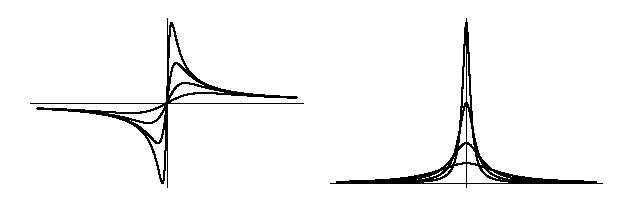
\includegraphics[width=0.8\textwidth]{fcv/residue/cpv_rii}
    \end{center}
    \caption{The real and imaginary part of the integrand for several values 
      of parameter.}
    \label{cpv_rii}
  \end{figure}

  Note that 
  \[
  \Re \int_0^1 \frac{1}{x - \imath \alpha} \,\dd x \to +\infty\ \mathrm{as}\ \alpha \to 0^+
  \]
  and
  \[
  \Re \int_{-1}^0 \frac{1}{x - \imath \alpha} \,\dd x \to -\infty\ \mathrm{as}\ \alpha \to 0^-.
  \]
  However,
  \[
  \lim_{\alpha \to 0} \Re \int_{-1}^1 \frac{1}{x - \imath \alpha} \,\dd x = 0
  \]
  because the two integrals above cancel each other.

  Now note that when $\alpha = 0$, the integrand is real.  Of course the 
  integral doesn't converge for this case, but if we could assign some 
  value to 
  \[
  \int_{-1}^1 \frac{1}{x} \,\dd x
  \]
  it would be a real number.  Since
  \[
  \lim_{\alpha \to 0} \int_{-1}^1 \Re \left[ \frac{1}{x - \imath \alpha} \right] \,\dd x
  = 0,
  \]
  This number should be zero.
\end{Solution}








%% Do the principal values of the following integrals exist?
\begin{Solution}
  \label{solution cpv 1/x^2}
  \begin{enumerate}
  \item
    \begin{align*}
      \pv \int_{-1}^1 \frac{1}{x^2} \,\dd x
      &= \lim_{\epsilon \to 0^+} \left(
        \int_{-1}^{-\epsilon} \frac{1}{x^2} \,\dd x
        + \int_\epsilon^1 \frac{1}{x^2} \,\dd x \right) \\
      &= \lim_{\epsilon \to 0^+} \left(
        \left[ -\frac{1}{x} \right]_{-1}^{-\epsilon}
        + \left[ -\frac{1}{x} \right]_\epsilon^1 \right) \\
      &= \lim_{\epsilon \to 0^+} \left(
        \frac{1}{\epsilon} -1 - 1 + \frac{1}{\epsilon} \right)
    \end{align*}
    The principal value of the integral does not exist.
  \item
    \begin{align*}
      \pv \int_{-1}^1 \frac{1}{x^3} \,\dd x
      &= \lim_{\epsilon \to 0^+} \left(
        \int_{-1}^{-\epsilon} \frac{1}{x^3} \,\dd x
        + \int_\epsilon^1 \frac{1}{x^3} \,\dd x \right) \\
      &= \lim_{\epsilon \to 0^+} \left(
        \left[ -\frac{1}{2x^2} \right]_{-1}^{-\epsilon}
        + \left[ -\frac{1}{2x^2} \right]_\epsilon^1 \right) \\
      &= \lim_{\epsilon \to 0^+} \left(
        -\frac{1}{2(-\epsilon)^2} +\frac{1}{2(-1)^2} 
        - \frac{1}{2(1)^2} + \frac{1}{2\epsilon^2} \right) \\
      &= 0
    \end{align*}
  \item
    Since $f(x)$ is real analytic, 
    \[
    f(x) = \sum_{n = 1}^\infty f_n x^n \quad \mathrm{for}\ x \in (-1,1).
    \]
    We can rewrite the integrand as
    \[
    \frac{f(x)}{x^3} = \frac{f_0}{x^3} + \frac{f_1}{x^2} + \frac{f_2}{x}
    + \frac{f(x)-f_0 -f_1 x - f_2 x^2}{x^3}.
    \]
    Note that the final term is real analytic on $(-1,1)$.  Thus the principal
    value of the integral exists if and only if $f_2 = 0$.
  \end{enumerate}
\end{Solution}





%%-----------------------------------------------------------------------------
\begin{large}
  \noindent
  \textbf{Cauchy Principal Value for Contour Integrals}
\end{large}



%% corner contour
\begin{Solution}
  \label{solution int ce f(z)}
  %% CONTINUE: Use the fundamental theorem of calculus instead.
  We can write $f(z)$ as
  \[
  f(z) = \frac{f_0}{z-z_0} + \frac{(z-z_0) f(z) - f_0}{z-z_0}.
  \]
  Note that the second term is analytic in a neighborhood of $z_0$.  Thus it
  is bounded on the contour.  Let $M_\epsilon$ be the maximum modulus of
  $\frac{(z-z_0) f(z) - f_0}{z-z_0}$ on $C_\epsilon$. 
  By using the maximum modulus integral bound, we have
  \begin{align*}
    \left| \int_{C_\epsilon} \frac{(z-z_0)f(z) -f_0}{z-z_0} \,\dd z \right|
    &\leq (\beta - \alpha) \epsilon M_\epsilon \\
    & \to 0 \quad \mathrm{as}\ \epsilon \to 0^+.
  \end{align*}
  Thus we see that
  \[
  \lim_{\epsilon \to 0^+} \int_{C_\epsilon} f(z) \,\dd z
  \lim_{\epsilon \to 0^+} \int_{C_\epsilon} \frac{f_0}{z-z_0} \,\dd z.
  \]
  We parameterize the path of integration with
  \[
  z = z_0 + \epsilon e^{\imath \theta}, \quad \theta \in (\alpha,\beta).
  \]
  Now we evaluate the integral.
  \begin{align*}
    \lim_{\epsilon \to 0^+} \int_{C_\epsilon} \frac{f_0}{z-z_0} \,\dd z
    &=\lim_{\epsilon \to 0^+} 
    \int_\alpha^\beta \frac{f_0}{\epsilon e^{\imath \theta}} 
    \imath \epsilon e^{\imath \theta}\,\dd \theta \\
    &=\lim_{\epsilon \to 0^+} 
    \int_\alpha^\beta \imath f_0 \,\dd \theta \\
    &= \imath (\beta - \alpha) f_0 \\
    &\equiv \imath (\beta - \alpha) \Res( f(z), z_0 )
  \end{align*}
  This proves the result.
\end{Solution}



%% residue theorem for principal values
\begin{Solution}
  \label{solution cpv res thrm}
  Let $C_i$ be the contour that is indented with circular arcs or radius
  $\epsilon$ at each of the first order poles on $C$ so as to enclose 
  these poles.  Let $A_1,\ldots,A_n$ be these circular arcs of radius
  $\epsilon$ centered at the points $\zeta_1,\ldots,\zeta_n$.  Let $C_p$ 
  be the contour, (not necessarily connected), obtained by subtracting 
  each of the $A_j$'s from $C_i$.

  Since the curve is $C^1$, (or continuously differentiable), at each of the
  first order poles on $C$, the $A_j$'s becomes semi-circles as 
  $\epsilon \to 0^+$.  Thus 
  \[
  \int_{A_j} f(z) \,\dd z = \imath \pi \Res(f(z),\zeta_j) \quad \mathrm{for}\ j = 1,\ldots,n.
  \]

  The principal value of the integral along $C$ is
  \begin{align*}
    \pv \int_C f(z) \,\dd z
    &= \lim_{\epsilon \to 0^+} \int_{C_p} f(z) \,\dd z \\
    &= \lim_{\epsilon \to 0^+} \left( \int_{C_i} f(z) \,\dd z -
      \sum_{j=1}^n \int_{A_j} f(z) \,\dd z \right) \\
    &= \imath 2 \pi \left( \sum_{j=1}^m \Res(f(z),z_j)
      + \sum_{j=1}^n \Res(f(z),\zeta_j) \right) -
    \imath \pi \sum_{j=1}^n \Res(f(z),\zeta_j) 
  \end{align*}
  \[
  \boxed{
    \pv \int_C f(z) \,\dd z = \imath 2 \pi \sum_{j=1}^m \Res(f(z),z_j)
    + \imath \pi \sum_{j=1}^n \Res(f(z),\zeta_j).
    }
  \]
\end{Solution}



%% \pv \int_C \frac{1}{z-1} \,\dd z
\begin{Solution}
  \label{solution 1/(z-1)}
  Consider 
  \[
  \pv \int_C \frac{1}{z-1} \,\dd z
  \]
  where $C$ is the unit circle.
  Let $C_p$ be the circular arc of radius 1 that starts and ends a distance
  of $\epsilon$ from $z=1$.  Let $C_\epsilon$ be the negative,
  circular arc of radius $\epsilon$ with center at $z=1$ that joins the endpoints
  of $C_p$.  Let $C_i$, be the union of $C_p$ and $C_\epsilon$.  ($C_p$ stands
  for Principal value Contour; $C_i$ stands for Indented Contour.)  $C_i$ is
  an indented contour that avoids the first order pole at $z=1$.  
  Figure~\ref{cpv_cicpceneg} shows the three contours.

  \begin{figure}[tb!]
    \begin{center}
      CONTINUE
      %%draw the picture
      \caption{The indented contour.}
      \label{cpv_cicpceneg}
    \end{center}
  \end{figure}

  Note that the principal value of the integral is
  \[
  \pv \int_C \frac{1}{z-1} \,\dd z
  = \lim_{\epsilon \to 0^+} \int_{C_p} \frac{1}{z-1} \,\dd z.
  \]
  We can calculate the integral along $C_i$ with Cauchy's theorem.  The 
  integrand is analytic inside the contour.
  \[
  \int_{C_i} \frac{1}{z-1} \,\dd z = 0
  \]
  We can calculate the integral along $C_\epsilon$ using Result~\ref{cpv_arcint}.
  Note that as $\epsilon \to 0^+$, the contour becomes a semi-circle, a 
  circular arc of $\pi$ radians in the negative direction.
  \[
  \lim_{\epsilon \to 0^+} \int_{C_\epsilon} \frac{1}{z-1} \,\dd z
  = - \imath \pi \Res\left( \frac{1}{z-1}, 1 \right) = - \imath \pi
  \]
  Now we can write the principal value of the integral along $C$ in terms of
  the two known integrals.
  \begin{align*}
    \pv \int_C \frac{1}{z-1} \,\dd z 
    &= \int_{C_i} \frac{1}{z-1} \,\dd z
    - \int_{C_\epsilon} \frac{1}{z-1} \,\dd z \\
    &= 0 - (-\imath \pi) \\
    &= \imath \pi
  \end{align*}
\end{Solution}




%%-----------------------------------------------------------------------------
\begin{large}
  \noindent
  \textbf{Integrals on the Real Axis}
\end{large}




\begin{Solution}
  \label{solution integrate x2 x2+1 x2+4}
  \begin{enumerate}
  \item 
    First we note that the integrand is an even function and extend the 
    domain of integration.
    \[
    \int_0^\infty \frac{x^2}{(x^2 + 1) (x^2 + 4)}\,\dd x
    = \frac{1}{2} \int_{-\infty}^\infty \frac{x^2}{(x^2 + 1) (x^2 + 4)}\,\dd x
    \]
    Next we close the path of integration in the upper half plane.
    Consider the integral along the boundary of the domain $0 < r < R$,
    $0 < \theta < \pi$.  
    \begin{align*}
      \frac{1}{2} \int_C \frac{z^2}{(z^2 + 1) (z^2 + 4)}\,\dd z
      &= \frac{1}{2} \int_C \frac{z^2}{(z - \imath) (z + \imath) (z - \imath 2) (z + \imath 2)}\,\dd z
      \\
      &= \imath 2 \pi \frac{1}{2} \bigg( 
      \Res\left( \frac{z^2}{(z^2 + 1) (z^2 + 4)}, z = \imath \right)
      \\
      &\qquad + \Res\left( \frac{z^2}{(z^2 + 1) (z^2 + 4)}, z = \imath 2 \right)
      \bigg)
      \\
      &= \imath \pi \left( 
        \left. \frac{z^2}{(z + \imath) (z^2 + 4)} \right|_{z = \imath}
        + \left. \frac{z^2}{(z^2 + 1) (z + \imath 2)} \right|_{z = \imath 2}
      \right)
      \\
      &= \imath \pi \left( \frac{\imath}{6} - \frac{\imath}{3} \right)
      \\
      &= \frac{\pi}{6}
    \end{align*}
    Let $C_R$ be the circular arc portion of the contour. $\int_C = \int_{-R}^R + \int_{C_R}$.
    We show that the integral along $C_R$ vanishes as $R \to \infty$ with the 
    maximum modulus bound.
    \begin{align*}
      \left| \int_{C_R} \frac{z^2}{(z^2 + 1) (z^2 + 4)}\,\dd z \right|
      &\leq \pi R \max_{z \in C_R} \left| \frac{z^2}{(z^2 + 1) (z^2 + 4)} \right|
      \\
      &= \pi R \frac{R^2}{(R^2 - 1) (R^2 - 4)}
      \\
      &\to 0\ \mathrm{as}\ R \to \infty
    \end{align*}
    We take the limit as $R \to \infty$ to evaluate the integral along the 
    real axis.
    \begin{gather*}
      \lim_{R \to \infty} \frac{1}{2} \int_{-R}^R \frac{x^2}{(x^2 + 1) (x^2 + 4)}\,\dd x 
      = \frac{\pi}{6}
      \\
      \int_0^\infty \frac{x^2}{(x^2 + 1) (x^2 + 4)}\,\dd x = \frac{\pi}{6}
    \end{gather*}
  \item 
    We close the path of integration in the upper half plane.
    Consider the integral along the boundary of the domain $0 < r < R$,
    $0 < \theta < \pi$.  
    \begin{align*}
      \int_C \frac{\dd z}{(z + b)^2 + a^2}
      &= \int_C \frac{\dd z}{(z + b - \imath a) (z + b + \imath a)}
      \\
      &= \imath 2 \pi \Res \left( \frac{1}{(z + b - \imath a) (z + b + \imath a)}, 
        z = -b + \imath a \right)
      \\
      &= \imath 2 \pi \left. \frac{1}{z + b + \imath a} \right|_{z = -b + \imath a}
      \\
      &= \frac{\pi}{a}
    \end{align*}
    Let $C_R$ be the circular arc portion of the contour. $\int_C = \int_{-R}^R + \int_{C_R}$.
    We show that the integral along $C_R$ vanishes as $R \to \infty$ with the 
    maximum modulus bound.
    \begin{align*}
      \left| \int_{C_R} \frac{\dd z}{(z + b)^2 + a^2} \right|
      &\leq \pi R \max_{z \in C_R} \left|  \frac{1}{(z + b)^2 + a^2} \right|
      \\
      &= \pi R \frac{1}{(R - b)^2 + a^2}
      \\
      &\to 0\ \mathrm{as}\ R \to \infty
    \end{align*}
    We take the limit as $R \to \infty$ to evaluate the integral along the 
    real axis.
    \begin{gather*}
      \lim_{R \to \infty} \int_{-R}^R \frac{\dd x}{(x + b)^2 + a^2} = \frac{\pi}{a}
      \\
      \int_{-\infty}^\infty \frac{\dd x}{(x + b)^2 + a^2} = \frac{\pi}{a}
    \end{gather*}
  \end{enumerate}
\end{Solution}









%% integrals from $-\infty$ to $\infty$
\begin{Solution}
  \label{solution int mii f(x)}
  Let $C_R$ be the semicircular arc from $R$ to $-R$ in the upper half plane.
  Let $C$ be the union of $C_R$ and the interval $[-R,R]$.  
  We can evaluate the principal value of the integral along $C$ with 
  Result~\ref{result residue theorem principal values}.
  \[
  \pv \int_C f(x) \,\dd x = \imath 2 \pi \sum_{k=1}^m \Res \left( f(z), z_k \right)
  + \imath \pi \sum_{k=1}^n \Res( f(z), x_k )
  \]
  We examine the integral along $C_R$ as $R \to \infty$.
  \begin{align*}
    \left| \int_{C_R} f(z) \,\dd z \right|
    &\leq \pi R \max_{z \in C_R} \left| f(z) \right| \\
    &\to 0 \quad \mathrm{as}\ R \to \infty.
  \end{align*}
  Now we are prepared to evaluate the real integral.
  \begin{align*}
    \pv \int_{-\infty}^\infty f(x) \,\dd x
    &= \lim_{R \to \infty} \pv \int_{-R}^R f(x) \,\dd x \\
    &= \lim_{R \to \infty} \pv \int_C f(z) \,\dd z \\
    &= \imath 2 \pi \sum_{k=1}^m \Res \left( f(z), z_k \right)
    + \imath \pi \sum_{k=1}^n \Res( f(z), x_k )
  \end{align*}
  If we close the path of integration in the lower half plane, the contour 
  will be in the negative direction.
  \[
  \pv \int_{-\infty}^\infty f(x) \,\dd x = - \imath 2 \pi \sum_{k=1}^m \Res \left( f(z), z_k \right)
  - \imath \pi \sum_{k=1}^n \Res( f(z), x_k )
  \]
\end{Solution}





%% \pv \int_{-\infty}^\infty \frac{2 x}{x^2 + x + 1}.
\begin{Solution}
  \label{solution 2x/(x^2+x+1)}
  We consider
  \[
  \pv \int_{-\infty}^\infty \frac{2 x}{x^2 + x + 1} \,\dd x.
  \]
  With the change of variables $x = 1/\xi$, this becomes
  \[
  \pv \int_\infty^{-\infty} \frac{2 \xi^{-1}}{ \xi^{-2} + \xi^{-1} + 1 }
  \left( \frac{-1}{\xi^2} \right) \,\dd \xi,
  \]
  \[
  \pv \int_{-\infty}^\infty \frac{2 \xi^{-1}}{ \xi^2 + \xi + 1 }\,\dd \xi
  \]
  There are first order poles at $\xi = 0$ and $\xi = -1/2 \pm \imath \sqrt{3}/2$.
  We close the path of integration in the upper half plane with a semi-circle.
  Since the integrand decays like $\xi^{-3}$ the integrand along the 
  semi-circle vanishes as the radius tends to infinity.  The value 
  of the integral is thus
  \[
  \imath \pi \Res \left( \frac{2 z^{-1}}{z^2 + z + 1}, z = 0 \right)
  + \imath 2 \pi \Res \left( \frac{2 z^{-1}}{z^2 + z + 1}, 
    z = - \frac{1}{2} + \imath \frac{ \sqrt{3} }{2} \right)
  \]
  \[
  \imath \pi \lim_{z \to 0} \left( \frac{ 2 }{ z^2 + z + 1 } \right)
  + \imath 2 \pi \lim_{z \to (-1+\imath \sqrt{3})/2} 
  \left( \frac{ 2 z^{-1} }{ z + (1 + \imath \sqrt{3} )/2 } \right)
  \]
  \[
  \boxed{
    \pv \int_{-\infty}^\infty \frac{2 x}{x^2 + x + 1} \,\dd x = 
    - \frac{ 2 \pi }{ \sqrt{3} }
    }
  \]
\end{Solution}



%% \int_{-\infty}^\infty \frac{1}{x^4 + 1} \,\dd x, \qquad \int_{-\infty}^\infty \frac{x^2}{(x^2+1)^2}\,\dd x.
\begin{Solution}
  \label{solution 1/(x^4+1)}
  \begin{enumerate}
    %%
    %%
    %%
  \item
    Consider
    \[
    \int_{-\infty}^\infty \frac{1}{x^4 + 1} \,\dd x.
    \]
    The integrand $\frac{1}{z^4+1}$ is analytic on the real axis and has isolated
    singularities at the points 
    \[
    z = \{ \e^{\imath \pi / 4}, \e^{\imath 3 \pi / 4}, \e^{\imath 5 \pi / 4}, \e^{\imath 7 \pi / 4} \}.
    \]
    Let $C_R$ be the semi-circle of radius $R$ in the upper half plane.  Since 
    \[
    \lim_{R \to \infty} \left( R \max_{z \in C_R} \left| \frac{1}{z^4 + 1} \right|
    \right)
    = \lim_{R \to \infty} \left( R \frac{1}{R^4 - 1} \right) = 0,
    \]
    we can apply Result~\ref{result int mii f(x)}.
    \[
    \int_{-\infty}^\infty \frac{1}{x^4 + 1}\,\dd x = \imath 2 \pi \left(
      \Res\left( \frac{1}{z^4+1}, \e^{\imath \pi / 4} \right) +
      \Res\left( \frac{1}{z^4+1}, \e^{\imath 3 \pi / 4} \right) \right)
    \]
    The appropriate residues are,
    \begin{align*}
      \Res\left( \frac{1}{z^4+1}, \e^{\imath \pi / 4} \right)
      &= \lim_{z \to \e^{\imath \pi / 4}} \frac{z - \e^{\imath \pi / 4}}{z^4+1} \\
      &= \lim_{z \to \e^{\imath \pi / 4}} \frac{1}{4 z^3} \\
      &= \frac{1}{4} \e^{- \imath 3 \pi / 4} \\
      &= \frac{-1 - \imath}{4 \sqrt{2}},
    \end{align*}
    \begin{align*}
      \Res\left( \frac{1}{z^4+1}, \e^{\imath 3 \pi / 4} \right)
      &= \frac{1}{4 (\e^{\imath 3 \pi / 4})^3} \\
      &= \frac{1}{4} \e^{- \imath \pi / 4} \\
      &= \frac{1 - \imath}{4 \sqrt{2}},
    \end{align*}
    We evaluate the integral with the residue theorem.
    \[
    \int_{-\infty}^\infty \frac{1}{x^4 + 1}\,\dd x = \imath 2 \pi \left( \frac{-1 - \imath}{4 \sqrt{2}}
      + \frac{1 - \imath}{4 \sqrt{2}} \right)
    \]
    \[
    \boxed{
      \int_{-\infty}^\infty \frac{1}{x^4 + 1}\,\dd x = \frac{\pi}{\sqrt{2}}
      }
    \]
    %%
    %%
    %%
  \item
    Now consider
    \[
    \int_{-\infty}^\infty \frac{x^2}{(x^2 + 1)^2} \,\dd x.
    \]
    The integrand is analytic on the real axis and has second order poles at
    $z = \pm \imath$.  Since the integrand decays sufficiently fast at infinity,
    \[
    \lim_{R \to \infty} \left( R \max_{z \in C_R} \left| \frac{z^2}{(z^2 + 1)^2} \right| \right)
    = \lim_{R \to \infty} \left( R \frac{R^2}{(R^2-1)^2} \right) = 0
    \]
    we can apply Result~\ref{result int mii f(x)}.
    \[
    \int_{-\infty}^\infty \frac{x^2}{(x^2 + 1)^2} \,\dd x
    = \imath 2 \pi \Res\left( \frac{z^2}{(z^2+1)^2}, z  = \imath \right)
    \]
    \begin{align*}
      \Res\left( \frac{z^2}{(z^2+1)^2}, z  = \imath \right)
      &= \lim_{z \to \imath} \frac{\dd}{\dd z} \left( 
        (z - \imath)^2 \frac{z^2}{(z^2+1)^2} \right) \\
      &= \lim_{z \to \imath} \frac{\dd}{\dd z} \left( \frac{z^2}{(z + \imath)^2} \right) \\
      &= \lim_{z \to \imath} \left( 
        \frac{(z + \imath)^2 2 z - z^2 2(z + \imath)}{(z + \imath)^4} \right) \\
      &= - \frac{\imath}{4}
    \end{align*}
    \[
    \boxed{
      \int_{-\infty}^\infty \frac{x^2}{(x^2 + 1)^2} \,\dd x = \frac{\pi}{2}
      }
    \]
    %%
    %%
    %%
  \item
    Since 
    \[
    \frac{\sin(x)}{1+x^2}
    \]
    is an odd function,
    \[
    \int_{-\infty}^\infty \frac{\cos(x)}{1+x^2} \,\dd x
    = \int_{-\infty}^\infty \frac{\e^{\imath x}}{1+x^2} \,\dd x
    \]
    Since $\e^{\imath z} / (1 + z^2)$ is analytic except for simple poles at $z = \pm \imath$ 
    and the integrand decays sufficiently fast in the upper half plane,
    \[
    \lim_{R \to \infty} \left( R \max_{z \in C_R} \left| \frac{\e^{\imath z}}{1+z^2} \right| \right)
    = \lim_{R \to \infty} \left( R \frac{1}{R^2 - 1} \right) = 0
    \]
    we can apply Result~\ref{result int mii f(x)}.
    \begin{align*}
      \int_{-\infty}^\infty \frac{\e^{\imath x}}{1+x^2} \,\dd x
      &= \imath 2 \pi \Res \left( \frac{\e^{\imath z}}{(z - \imath)(z + \imath)}, z = \imath \right) \\
      &= \imath 2 \pi \frac{\e^{-1}}{\imath 2}
    \end{align*}
    \[
    \boxed{
      \int_{-\infty}^\infty \frac{\cos(x)}{1+x^2} \,\dd x = \frac{\pi}{e}
      }
    \]
  \end{enumerate}
\end{Solution}










%% \int_0^\infty \frac{ x^6 }{ (x^4 + 1)^2 } \,\dd x.
\begin{Solution}
  \label{solution x^6/(x^4+1)^2}
  Consider the function 
  \[
  f(z) = \frac{ z^6 }{ (z^4 + 1)^2 }.
  \]
  The value of the function on the imaginary axis:
  \[
  \frac{ -y^6 }{ (y^4 + 1)^2 }
  \]
  is a constant multiple of the value of the function on the real axis:
  \[
  \frac{ x^6 }{ (x^4 + 1)^2 }.
  \]
  Thus to evaluate the real integral we consider the path of integration, $C$,
  which starts at the origin, follows the real axis to $R$, follows a 
  circular path to $\imath R$ and then follows the imaginary axis back down to 
  the origin.  $f(z)$ has second order poles at the fourth roots of $-1$: 
  $(\pm 1 \pm \imath) / \sqrt{2}$.  Of these only $(1 + \imath) / \sqrt{2}$
  lies inside the path of integration.  We evaluate the contour integral
  with the Residue Theorem.  For $R > 1$:
  \begin{align*}
    \int_C \frac{ z^6 }{ (z^4 + 1)^2 } \,\dd z
    &= \imath 2 \pi \Res \left( \frac{ z^6 }{ (z^4 + 1)^2 }, z = \e^{\imath \pi / 4}
    \right) \\
    &= \imath 2 \pi \lim_{z \to \e^{\imath \pi / 4} } \frac{\dd}{\dd z} \left(
      (z - \e^{\imath \pi / 4})^2 \frac{ z^6 } { (z^4 + 1)^2 } \right) \\
    &= \imath 2 \pi \lim_{z \to \e^{\imath \pi / 4} } \frac{\dd}{\dd z} \left(
      \frac{ z^6 } { (z - \e^{\imath 3 \pi / 4})^2
        (z - \e^{\imath 5 \pi / 4})^2 (z - \e^{\imath 7 \pi / 4})^2 } \right) \\
    &= \imath 2 \pi \lim_{z \to \e^{\imath \pi / 4} } \Bigg(
    \frac{ z^6 }{ (z - \e^{\imath 3 \pi / 4})^2
      (z - \e^{\imath 5 \pi / 4})^2 (z - \e^{\imath 7 \pi / 4})^2 } \\
    &\qquad \left( \frac{6}{z} - \frac{2}{z - \e^{\imath 3 \pi / 4} }
      - \frac{2}{z - \e^{\imath 5 \pi / 4} }
      - \frac{2}{z - \e^{\imath 7 \pi / 4} }
    \right) \Bigg) \\
    &= \imath 2 \pi \frac{ -\imath }{ (2)(\imath 4)(-2) } \left( 
      \frac{6 \sqrt{2} }{ 1 + \imath } - \frac{ 2 }{ \sqrt{2} }
      - \frac{ 2 \sqrt{2} }{ 2 + \imath 2 } - \frac{ 2 }{ \imath \sqrt{2} }
    \right) \\
    &= \imath 2 \pi \frac{3}{32} (1 - \imath) \sqrt{2} \\
    &= \frac{3 \pi }{ 8 \sqrt{2} } (1 + \imath)
  \end{align*}
  The integral along the circular part of the contour, $C_R$, vanishes as 
  $R \to \infty$.  We demonstrate this with the maximum modulus integral 
  bound.
  \begin{align*}
    \left| \int_{C_R} \frac{ z^6 }{ (z^4 + 1)^2 } \,\dd z \right| 
    &\leq \frac{\pi R}{4} \max_{z \in C_R} 
    \left( \frac{ z^6 }{ (z^4 + 1)^2 } \right) \\
    &= \frac{\pi R}{4} \frac{ R^6 }{ (R^4 - 1)^2 } \\
    &\to 0\ \mathrm{as}\ R \to \infty
  \end{align*}
  Taking the limit $R \to \infty$, we have:
  \begin{gather*}
    \int_0^\infty \frac{ x^6 }{ (x^4 + 1)^2 } \,\dd x
    + \int_{\infty}^0 \frac{ (\imath y)^6 }{ ((\imath y)^4 + 1)^2 } \imath \,\dd y
    = \frac{3 \pi }{ 8 \sqrt{2} } (1 + \imath) \\
    \int_0^\infty \frac{ x^6 }{ (x^4 + 1)^2 } \,\dd x
    + \imath  \int_0^\infty \frac{ y^6 }{ (y^4 + 1)^2 } \,\dd y
    = \frac{3 \pi }{ 8 \sqrt{2} } (1 + \imath) \\
    (1 + \imath) \int_0^\infty \frac{ x^6 }{ (x^4 + 1)^2 } \,\dd x
    = \frac{3 \pi }{ 8 \sqrt{2} } (1 + \imath) \\
    \boxed{
      \int_0^\infty \frac{ x^6 }{ (x^4 + 1)^2 } \,\dd x
      = \frac{3 \pi }{ 8 \sqrt{2} } 
      }
  \end{gather*}
\end{Solution}





%%-----------------------------------------------------------------------------
\begin{large}
  \noindent
  \textbf{Fourier Integrals}
\end{large}



%% jordan's lemma
\begin{Solution}
  \label{solution jordan's lemma}
  We know that
  \[
  \int_0^\pi \e^{-R \sin\theta} \,\dd \theta < \frac{\pi}{R}.
  \]
  First take the case that $\omega$ is positive and the semi-circle is in the
  upper half plane.
  \begin{align*}
    \left| \int_{C_R} f(z)  \e^{\imath \omega z} \,\dd z \right|
    &\leq \left| \int_{C_R} \e^{\imath \omega z} \,\dd z \right|
    \max_{z \in C_R} |f(z)| \\
    &\leq \int_0^\pi \left| \e^{\imath \omega R \e^{\imath \theta}} 
      R \e^{\imath \theta} \right| \,\dd \theta 
    \max_{z \in C_R} |f(z)| \\
    &= R \int_0^\pi \left| \e^{- \omega R \sin \theta} \right| \,\dd \theta 
    \max_{z \in C_R} |f(z)| \\
    &< R \frac{\pi}{\omega R}
    \max_{z \in C_R} |f(z)| \\
    &= \frac{\pi}{\omega}
    \max_{z \in C_R} |f(z)| \\
    &\to 0 \quad \mathrm{as}\ R \to \infty
  \end{align*}
  The procedure is almost the same for negative $\omega$.
\end{Solution}






%% \int_{-\infty}^\infty \frac{ \cos 2 x }{ x - \imath \pi } \,\dd x.
\begin{Solution}
  \label{solution cos(2x)/(x-i pi)}
  First we write the integral in terms of Fourier integrals.
  \[
  \int_{-\infty}^\infty \frac{ \cos 2 x }{ x - \imath \pi } \,\dd x
  = \int_{-\infty}^\infty \frac{ \e^{\imath 2 x} }{ 2 (x - \imath \pi) } \,\dd x
  + \int_{-\infty}^\infty \frac{ \e^{-\imath 2 x} }{ 2 (x - \imath \pi) } \,\dd x
  \]
  Note that $\frac{1}{2 (z - \imath \pi) }$ vanishes as $|z| \to \infty$.
  We close the former Fourier integral in the upper half plane and the 
  latter in the lower half plane.
  There is a first order pole at $z = \imath \pi$ in the upper half plane.
  \begin{align*}
    \int_{-\infty}^\infty \frac{ \e^{\imath 2 x} }{ 2 (x - \imath \pi) } \,\dd x
    &= \imath 2 \pi \Res \left( \frac{ \e^{\imath 2 z} }{ 2 (z - \imath \pi) },
      z = \imath \pi \right) \\
    &= \imath 2 \pi \frac{ \e^{-2 \pi} }{ 2 }
  \end{align*}
  There are no singularities in the lower half plane.
  \[
  \int_{-\infty}^\infty \frac{ \e^{-\imath 2 x} }{ 2 (x - \imath \pi) } \,\dd x = 0
  \]
  Thus the value of the original real integral is
  \[
  \boxed{
    \int_{-\infty}^\infty \frac{ \cos 2 x }{ x - \imath \pi } \,\dd x = \imath \pi \e^{-2 \pi}
    }
  \]
\end{Solution}









%%-----------------------------------------------------------------------------
\begin{large}
  \noindent
  \textbf{Fourier Cosine and Sine Integrals}
\end{large}




%% \int_{-\infty}^\infty \frac{\sin x}{x} \,\dd x.
\begin{Solution}
  \label{solution sin(x)/x}
  We are considering the integral
  \[
  \int_{-\infty}^\infty \frac{\sin x}{x} \,\dd x.
  \]
  The integrand is an entire function.  So it doesn't appear that the residue
  theorem would directly apply. Also the integrand is unbounded as 
  $x \to + \imath \infty$ and $x \to - \imath \infty$, so closing the integral in the
  upper or lower half plane is not directly applicable.  In order to proceed,
  we must write the integrand in a different form.
  Note that
  \[
  \pv \int_{-\infty}^\infty \frac{\cos x}{x} \,\dd x = 0
  \]
  since the integrand is odd and has only a first order pole at $x = 0$.
  Thus
  \[
  \int_{-\infty}^\infty \frac{\sin x}{x} \,\dd x
  = \pv \int_{-\infty}^\infty \frac{e^{\imath x}}{\imath x} \,\dd x.
  \]
  Let $C_R$ be the semicircular arc in the upper half plane from $R$ to $-R$.
  Let $C$ be the closed contour that is the union of $C_R$ and the real interval
  $[-R,R]$.
  If we close the path of integration with a semicircular arc in the upper
  half plane, we have
  \[
  \int_{-\infty}^\infty \frac{\sin x}{x} \,\dd x
  = \lim_{R \to \infty} \left( \pv \int_C \frac{e^{\imath z}}{\imath z} \,\dd z
    - \int_{C_R} \frac{e^{\imath z}}{\imath z} \,\dd z \right),
  \]
  provided that all the integrals exist.

  The integral along $C_R$ vanishes as $R \to \infty$ by Jordan's lemma.
  By the residue theorem for principal values we have
  \[
  \pv \int \frac{e^{\imath z}}{\imath z} \,\dd z = \imath \pi \Res\left( \frac{e^{\imath z}}{\imath z}, 0
  \right) = \pi.
  \]
  Combining these results,
  \[
  \boxed{
    \int_{-\infty}^\infty \frac{\sin x}{x} \,\dd x = \pi.
    }
  \]
\end{Solution}



%% \int_{-\infty}^\infty \frac{1 - \cos x}{x^2} \,\dd x.
\begin{Solution}
  \label{solution (1-cos x)/x^2}
  Note that $(1 - \cos x)/x^2$ has a removable singularity at $x = 0$.
  The integral decays like $\frac{1}{x^2}$ at infinity, so the integral 
  exists.
  Since $(\sin x)/x^2$ is a odd function with a simple pole at $x = 0$,
  the principal value of its integral vanishes.
  \begin{gather*}
    \pv \int_{-\infty}^\infty \frac{\sin x}{x^2}\,\dd x = 0 \\
    \int_{-\infty}^\infty \frac{1 - \cos x}{x^2}\,\dd x 
    = \pv \int_{-\infty}^\infty \frac{1 - \cos x - \imath \sin x}{x^2}\,\dd x
    = \pv \int_{-\infty}^\infty \frac{1 - \e^{\imath x}}{x^2}\,\dd x
  \end{gather*}
  Let $C_R$ be the semi-circle of radius $R$ in the upper half plane.
  Since
  \[
  \lim_{R \to \infty} \left( R \max_{z \in C_R} \left| \frac{1 - \e^{\imath z}}{z^2} \right| \right)
  = \lim_{R \to \infty} R \frac{2}{R^2} = 0
  \]
  the integral along $C_R$ vanishes as $R \to \infty$.  
  \[
  \int_{C_R} \frac{1 - \e^{\imath z}}{z^2}\,\dd z \to 0\ \mathrm{as}\ R \to \infty
  \]
  We can apply Result~\ref{result int mii f(x)}.
  \[
  \pv \int_{-\infty}^\infty \frac{1 - \e^{\imath x}}{x^2}\,\dd x
  = \imath \pi \Res \left( \frac{1 - \e^{\imath z}}{z^2}, z = 0 \right)
  = \imath \pi \lim_{z \to 0} \frac{1 - \e^{\imath z}}{z}
  = \imath \pi \lim_{z \to 0} \frac{-\imath \e^{\imath z}}{1}
  \]
  \[
  \boxed{
    \int_{-\infty}^\infty \frac{1 - \cos x}{x^2}\,\dd x = \pi
    }
  \]
\end{Solution}



%% \int_0^\infty \frac{\sin(\pi x)}{x(1-x^2)} \,\dd x.
\begin{Solution}
  \label{solution sin(pi x)/(x(1-x^2))}
  Consider
  \[
  \int_0^\infty \frac{\sin(\pi x)}{x(1-x^2)}\,\dd x.
  \]
  Note that the integrand has removable singularities at the points 
  $x = 0,\pm 1$ and is an even function.
  \[
  \int_0^\infty \frac{\sin(\pi x)}{x(1-x^2)}\,\dd x
  = \frac{1}{2} \int_{-\infty}^\infty \frac{\sin(\pi x)}{x(1-x^2)}\,\dd x.
  \]
  Note that $\displaystyle \frac{\cos(\pi x)}{x(1-x^2)}$ 
  is an odd function with first order poles at $x = 0,\pm 1$.
  \begin{gather*}
    \pv \int_{-\infty}^\infty \frac{\cos(\pi x)}{x(1-x^2)}\,\dd x = 0 \\
    \int_0^\infty \frac{\sin(\pi x)}{x(1-x^2)}\,\dd x
    = - \frac{\imath}{2} \pv \int_{-\infty}^\infty \frac{\e^{\imath \pi x}}{x(1-x^2)}\,\dd x.
  \end{gather*}
  Let $C_R$ be the semi-circle of radius $R$ in the upper half plane.
  Since
  \[
  \lim_{R \to \infty} \left( R \max_{z \in C_R} \left| \frac{\e^{\imath \pi z}}{z(1-z^2)} \right| \right)
  = \lim_{R \to \infty} R \frac{1}{R(R^2-1)} = 0
  \]
  the integral along $C_R$ vanishes as $R \to \infty$.  
  \[
  \int_{C_R} \frac{\e^{\imath \pi z}}{z(1-z^2)} \,\dd z \to 0\ \mathrm{as}\ R \to \infty
  \]
  We can apply Result~\ref{result int mii f(x)}.
  \begin{align*}
    - \frac{\imath}{2} \pv \int_{-\infty}^\infty \frac{\e^{\imath \pi x}}{x(1-x^2)}\,\dd x
    &= \imath \pi \frac{-\imath}{2} \bigg(
    \Res \left( \frac{\e^{\imath z}}{z(1-z^2)}, z = 0 \right)
    + \Res \left( \frac{\e^{\imath z}}{z(1-z^2)}, z = 1 \right) \\
    & \qquad \qquad + \Res \left( \frac{\e^{\imath z}}{z(1-z^2)}, z = -1 \right)
    \bigg) \\
    &= \frac{\pi}{2} \left(
      \lim_{z \to 0} \frac{\e^{\imath \pi z}}{1-z^2}
      - \lim_{z \to 0} \frac{\e^{\imath \pi z}}{z(1+z)}
      + \lim_{z \to 0} \frac{\e^{\imath \pi z}}{z(1-z)} \right) \\
    &= \frac{\pi}{2} \left( 1 - \frac{-1}{2} + \frac{-1}{-2} \right)
  \end{align*}
  \[
  \boxed{
    \int_0^\infty \frac{\sin(\pi x)}{x(1-x^2)}\,\dd x = \pi
    }
  \]
\end{Solution}



%%-----------------------------------------------------------------------------
\begin{large}
  \noindent
  \textbf{Contour Integration and Branch Cuts}
\end{large}
















\begin{Solution}
  \label{solution int (ln x)^2 / (1 + x^2)}
  Let $C$ be the boundary of the region $\epsilon < r < R$, $0 < \theta < \pi$.  Choose the 
  branch of the logarithm with a branch cut on the negative imaginary axis
  and the angle range $-\pi / 2 < \theta < 3 \pi / 2$.  We consider the integral of
  $\log^2 z / (1 + z^2)$ on this contour.
  \begin{align*}
    \oint_C \frac{\log^2 z}{1 + z^2}\,\dd z
    &= \imath 2 \pi \Res \left( \frac{\log^2 z}{1 + z^2}, z = \imath \right) 
    \\
    &= \imath 2 \pi \lim_{z \to \imath} \frac{\log^2 z}{z + \imath} 
    \\
    &= \imath 2 \pi \frac{(\imath \pi / 2)^2}{\imath 2}
    \\
    &= - \frac{\pi^3}{4}
  \end{align*}
  Let $C_R$ be the semi-circle from $R$ to $-R$ in the upper half plane.
  We show that the integral along $C_R$ vanishes as $R \to \infty$ with the maximum
  modulus integral bound.
  \begin{align*}
    \left| \int_{C_R} \frac{\log^2 z}{1 + z^2}\,\dd z \right|
    &\leq \pi R \max_{z \in C_R} \left| \frac{\log^2 z}{1 + z^2} \right|
    \\
    &\leq \pi R \frac{\ln^2 R + 2 \pi \ln R + \pi^2}{R^2 - 1} 
    \\
    &\to 0\ \mathrm{as}\ R \to \infty 
  \end{align*}
  Let $C_\epsilon$ be the semi-circle from $-\epsilon$ to $\epsilon$ in the upper half plane.
  We show that the integral along $C_\epsilon$ vanishes as $\epsilon \to 0$ with the maximum
  modulus integral bound.
  \begin{align*}
    \left| \int_{C_\epsilon} \frac{\log^2 z}{1 + z^2}\,\dd z \right|
    &\leq \pi \epsilon \max_{z \in C_\epsilon} \left| \frac{\log^2 z}{1 + z^2} \right|
    \\
    &\leq \pi \epsilon \frac{\ln^2 \epsilon - 2 \pi \ln \epsilon + \pi^2}{1 - \epsilon^2}
    \\
    &\to 0\ \mathrm{as}\ \epsilon \to 0
  \end{align*}

  Now we take the limit as $\epsilon \to 0$ and $R \to \infty$ for the integral along $C$.
  \begin{gather}
    \nonumber
    \oint_C \frac{\log^2 z}{1 + z^2}\,\dd z = - \frac{\pi^3}{4} 
    \\
    \nonumber
    \int_0^\infty \frac{\ln^2 r}{1 + r^2}\,\dd r 
    + \int_\infty^0 \frac{(\ln r + \imath \pi)^2}{1 + r^2}\,\dd r 
    = - \frac{\pi^3}{4} 
    \\
    \label{equation int (ln x)^2 / (1 + x^2)}
    2 \int_0^\infty \frac{\ln^2 x}{1 + x^2}\,\dd x 
    + \imath 2 \pi \int_0^\infty \frac{\ln x}{1 + x^2}\,\dd x 
    = \pi^2 \int_0^\infty \frac{1}{1 + x^2}\,\dd x 
    - \frac{\pi^3}{4}
  \end{gather}

  We evaluate the integral of $1/(1 + x^2)$ by extending the path of integration
  to $(-\infty \ldots \infty)$ and closing the path of integration in the upper half plane.
  Since 
  \[
  \lim_{R \to \infty} \left( R \max_{z \in C_R} \left| \frac{1}{1 + z^2} \right| \right)
  \leq \lim_{R \to \infty} \left( R \frac{1}{R^2 - 1} \right) = 0,
  \]
  the integral of $1 / (1 + z^2)$ along $C_R$ vanishes as $R \to \infty$.  We evaluate 
  the integral with the Residue Theorem.
  \begin{align*}
    \pi^2 \int_0^\infty \frac{1}{1 + x^2}\,\dd x 
    &= \frac{\pi^2}{2} \int_{-\infty}^\infty \frac{1}{1 + x^2}\,\dd x
    \\
    &= \frac{\pi^2}{2} \imath 2 \pi \Res \left( \frac{1}{1 + z^2}, z = \imath \right) 
    \\
    &= \imath \pi^3 \lim_{z \to \imath} \frac{1}{z + \imath} 
    \\
    &= \frac{\pi^3}{2}
  \end{align*}

  Now we return to Equation~\ref{equation int (ln x)^2 / (1 + x^2)}.
  \[
  2 \int_0^\infty \frac{\ln^2 x}{1 + x^2}\,\dd x 
  + \imath 2 \pi \int_0^\infty \frac{\ln x}{1 + x^2} \,\dd x 
  = \frac{\pi^3}{4}
  \]
  We equate the real and imaginary parts to solve for the desired integrals.
  \begin{gather*}
    \boxed{
      \int_0^\infty \frac{\ln^2 x}{1 + x^2} \,\dd x = \frac{\pi^3}{8}
      } \\
    \boxed{
      \int_0^\infty \frac{\ln x}{1 + x^2} \,\dd x = 0
      }
  \end{gather*}
\end{Solution}















%% \int_0^\infty \frac{\dd x}{ x^2 + 5 x + 6 }
\begin{Solution}
  \label{solution 1/(x^2+5x+6)}
  We consider the branch of the function
  \[
  f(z) = \frac{ \log z }{ z^2 + 5 z + 6 }
  \]
  with a branch cut on the real axis and $0 < \arg(z) < 2 \pi$.

  Let $C_\epsilon$ and $C_R$ denote the circles of radius $\epsilon$ and $R$
  where $\epsilon < 1 < R$.  $C_\epsilon$ is negatively oriented;
  $C_R$ is positively oriented.
  Consider the closed contour, $C$, that is traced by a point moving from
  $\epsilon$ to $R$ above the branch cut, next around $C_R$ back to $R$, then
  below the cut to $\epsilon$, and finally around $C_\epsilon$ back to $\epsilon$.
  (See Figure~\ref{contepsr z2+5z+6}.)
  \begin{figure}[tb!]
    \begin{center}
      \includegraphics[width=0.25\textwidth]{fcv/residue/contepsr}
    \end{center}
    \caption{The path of integration.}
    \label{contepsr z2+5z+6}
  \end{figure}

  We can evaluate the integral of $f(z)$ along $C$ with the residue theorem.
  For $R > 3$, there are first order poles inside the path of integration 
  at $z = -2$ and $z = -3$.
  \begin{align*}
    \int_C \frac{ \log z }{ z^2 + 5 z + 6 } \,\dd z
    &= \imath 2 \pi \left( \Res \left( \frac{ \log z }{ z^2 + 5 z + 6 },
        z = -2 \right)
      + \Res \left( \frac{ \log z }{ z^2 + 5 z + 6 }, z = -3 \right)
    \right) \\
    &= \imath 2 \pi \left( \lim_{z \to -2} \frac{ \log z }{ z + 3 }
      + \lim_{z \to -3} \frac{ \log z }{ z + 2 } \right) \\
    &= \imath 2 \pi \left( \frac{ \log(-2) }{ 1 } + \frac{ \log(-3) }{ -1 }
    \right) \\
    &= \imath 2 \pi \left( \log(2) + \imath \pi - \log(3) - \imath \pi \right) \\
    &= \imath 2 \pi \log \left( \frac{2}{3} \right)
  \end{align*}

  In the limit as $\epsilon \to 0$, the integral along $C_\epsilon$ vanishes.
  We demonstrate this with the maximum modulus theorem.
  \begin{align*}
    \left| \int_{C_\epsilon} \frac{ \log z }{ z^2 + 5 z + 6 }\,\dd  z \right|
    &\leq 2 \pi \epsilon \max_{z \in C_\epsilon} 
    \left| \frac{ \log z }{ z^2 + 5 z + 6 } \right| \\
    &\leq 2 \pi \epsilon \frac{ 2 \pi - \log \epsilon }
    { 6 - 5 \epsilon - \epsilon^2 } \\
    &\to 0\ \mathrm{as}\ \epsilon \to 0
  \end{align*}

  In the limit as $R \to \infty$, the integral along $C_R$ vanishes.
  We again demonstrate this with the maximum modulus theorem.
  \begin{align*}
    \left| \int_{C_R} \frac{ \log z }{ z^2 + 5 z + 6 }\,\dd  z \right|
    &\leq 2 \pi R \max_{z \in C_R} 
    \left| \frac{ \log z }{ z^2 + 5 z + 6 } \right| \\
    &\leq 2 \pi R \frac{ \log R + 2 \pi }
    { R^2 - 5 R - 6 } \\
    &\to 0\ \mathrm{as}\ R \to \infty
  \end{align*}

  Taking the limit as $\epsilon \to 0$ and $R \to \infty$, the integral
  along $C$ is:
  \begin{align*}
    \int_C \frac{ \log z }{ z^2 + 5 z + 6 } \,\dd z
    &= \int_0^\infty \frac{ \log x }{ x^2 + 5 x + 6 } \,\dd x
    + \int_{\infty}^0 \frac{ \log x + \imath 2 \pi }{ x^2 + 5 x + 6 } \,\dd x \\
    &= -\imath 2 \pi \int_0^\infty \frac{ \log x }{ x^2 + 5 x + 6 } \,\dd x
  \end{align*}
  Now we can evaluate the real integral.
  \begin{gather*}
    -\imath 2 \pi \int_0^\infty \frac{ \log x }{ x^2 + 5 x + 6 } \,\dd x
    = \imath 2 \pi \log \left( \frac{2}{3} \right) \\
    \boxed{
      \int_0^\infty \frac{ \log x }{ x^2 + 5 x + 6 } \,\dd x
      = \log \left( \frac{3}{2} \right)
      }
  \end{gather*}
\end{Solution}







%% \int_0^\infty \frac{x^a}{(x+1)^2}\,\dd x 
\begin{Solution}
  \label{solution x^a/(x+1)^2}
  We consider the integral
  \[
  I(a) = \int_0^\infty \frac{x^a}{(x+1)^2}\,\dd x.
  \]
  To examine convergence, we split the domain of integration.
  \[
  \int_0^\infty \frac{x^a}{(x+1)^2}\,\dd x
  = \int_0^1 \frac{x^a}{(x+1)^2}\,\dd x
  + \int_1^\infty \frac{x^a}{(x+1)^2}\,\dd x
  \]

  First we work with the integral on $(0 \ldots 1)$.
  \begin{align*}
    \left| \int_0^1 \frac{x^a}{(x+1)^2}\,\dd x \right|
    &\leq \int_0^1 \left| \frac{x^a}{(x+1)^2} \right| 
     \left| d x \right| \\
    &= \int_0^1 \frac{x^{\Re(a)}}{(x+1)^2} \,\dd x \\
    &\leq \int_0^1 x^{\Re(a)} \,\dd x
  \end{align*}
  This integral converges for $\Re(a) > -1$.

  Next we work with the integral on $(1 \ldots \infty)$.
  \begin{align*}
    \left| \int_1^\infty \frac{x^a}{(x+1)^2}\,\dd x \right|
    &\leq \int_1^\infty \left| \frac{x^a}{(x+1)^2} \right| 
     \left| d x \right| \\
    &= \int_1^\infty \frac{x^{\Re(a)}}{(x+1)^2} \,\dd x \\
    &\leq \int_1^\infty x^{\Re(a) - 2} \,\dd x
  \end{align*}
  This integral converges for $\Re(a) < 1$.

  Thus we see that the integral defining $I(a)$ converges in the 
  strip,  $-1 < \Re(a) < 1$.  The integral converges uniformly in any closed
  subset of this domain.  Uniform convergence means that we can differentiate
  the integral with respect to $a$ and interchange the order of 
  integration and differentiation.
  \[
  I'(a) = \int_0^\infty \frac{x^a \log x}{(x+1)^2}\,\dd x
  \]
  Thus we see that $I(a)$ is analytic for $-1 < \Re(a) < 1$.

  For $-1 < \Re(a) < 1$ and $a \neq 0$, $z^a$ is multi-valued.
  Consider the branch of the function $f(z) = z^a / (z+1)^2$ with a 
  branch cut on the positive real axis and $0 < \arg(z) < 2 \pi$.
  We integrate along the contour in Figure~\ref{contepsr}.

  The integral on $C_\epsilon$ vanishes as $\epsilon \to 0$.  We show this 
  with the maximum modulus integral bound.
  First we write $z^a$ in modulus-argument form, $z = \epsilon \e^{\imath \theta}$,
  where $a = \alpha + \imath \beta$.
  \begin{align*}
    z^a     &= \e^{a \log z} \\
    &= \e^{ (\alpha + \imath \beta) (\ln \epsilon + \imath \theta) } \\
    &= \e^{ \alpha \ln \epsilon - \beta \theta + \imath ( \beta \ln \epsilon + \alpha \theta ) } \\
    &= \epsilon^\alpha \e^{ - \beta \theta } \e^{ \imath ( \beta \log \epsilon + \alpha \theta ) } \\
  \end{align*}
  Now we bound the integral.
  \begin{align*}
    \left| \int_{C_\epsilon} \frac{z^a}{(z+1)^2}\,\dd z \right|
    &\leq 2 \pi \epsilon \max_{z \in C_\epsilon} \left| \frac{z^a}{(z+1)^2} \right| \\
    &\leq 2 \pi \epsilon \frac{ \epsilon^\alpha \e^{ 2 \pi |\beta|} }{(1-\epsilon)^2}\\
    &\to 0\ \mathrm{as}\ \epsilon \to 0
  \end{align*}

  The integral on $C_R$ vanishes as $R \to \infty$.
  \begin{align*}
    \left| \int_{C_R} \frac{z^a}{(z+1)^2}\,\dd z \right|
    &\leq 2 \pi R \max_{z \in C_R} \left|
      \frac{z^a}{(z+1)^2} \right| \\
    &\leq 2 \pi R \frac{ R^\alpha \e^{2 \pi |\beta|} }{(R-1)^2} \\
    &\to 0\ \mathrm{as}\ R \to \infty
  \end{align*}

  Above the branch cut, ($z = r \e^{\imath 0}$), the integrand is
  \[
  f(r \e^{\imath 0}) = \frac{r^a}{(r+1)^2}.
  \]
  Below the branch cut, ($z = r \e^{\imath 2 \pi}$), we have,
  \[
  f(r \e^{\imath 2 \pi}) = \frac{\e^{\imath 2 \pi a} r^a}{(r+1)^2}.
  \]
  Now we use the residue theorem. 
  \begin{gather*}
    \int_0^\infty \frac{r^a}{(r+1)^2} \,\dd r 
    + \int_\infty^0 \frac{\e^{\imath 2 \pi a} r^a}{(r+1)^2}\,\dd r
    = \imath 2 \pi \Res \left( \frac{z^a}{(z+1)^2}, -1 \right) \\
    \left( 1 - \e^{\imath 2 \pi a} \right) \int_0^\infty \frac{r^a}{(r+1)^2} \,\dd r 
    = \imath 2 \pi \lim_{z \to -1}  \frac{\dd}{\dd z} (z^a) \\
    \int_0^\infty \frac{r^a}{(r+1)^2} \,\dd r 
    = \imath 2 \pi \frac{a \e^{\imath \pi (a-1)}}{ 1 - \e^{\imath 2 \pi a} } \\
    \int_0^\infty \frac{r^a}{(r+1)^2} \,\dd r 
    = \frac{- \imath 2 \pi a }{ \e^{- \imath \pi a}  - \e^{\imath \pi a} } \\
    \int_0^\infty \frac{x^a}{(x+1)^2} \,\dd x = \frac{ \pi a }{ \sin(\pi a) }
    \quad \mathrm{for}\ -1 < \Re(a) < 1,\ a \neq 0
  \end{gather*}
  The right side has a removable singularity at $a = 0$.  We use analytic
  continuation to extend the answer to $a = 0$.
  \[
  \boxed{
    I(a) = \int_0^\infty \frac{x^a}{(x+1)^2} \,\dd x = 
    \begin{cases}
      \frac{ \pi a }{ \sin(\pi a) } &\mathrm{for}\ -1 < \Re(a) < 1,\ a \neq 0 \\
      1 &\mathrm{for}\ a = 0
    \end{cases}
    }
  \]


  We can derive the last two integrals by differentiating this formula with 
  respect to $a$ and taking the limit $a \to 0$.  
  \begin{gather*}
    I'(a) = \int_0^\infty \frac{x^a \log x}{(x+1)^2}\,\dd x, \qquad
    I''(a) = \int_0^\infty \frac{x^a \log^2 x}{(x+1)^2}\,\dd x \\
    I'(0) = \int_0^\infty \frac{\log x}{(x+1)^2}\,\dd x, \qquad
    I''(0) = \int_0^\infty \frac{\log^2 x}{(x+1)^2}\,\dd x 
  \end{gather*}
  We can find $I'(0)$ and $I''(0)$ either by differentiating the 
  expression for $I(a)$ or by finding the first few terms in the 
  Taylor series expansion of $I(a)$ about $a = 0$.  The latter approach
  is a little easier.
  \[
  I(a) = \sum_{n = 0}^\infty \frac{ I^{(n)}(0) }{ n! } a^n
  \]
  \begin{align*}
    I(a)    &= \frac{\pi a}{\sin (\pi a)} \\
    &= \frac{\pi a}{ \pi a - (\pi a)^3 / 6 + \mathcal{O}(a^5) } \\
    &= \frac{1}{1 - (\pi a)^2 / 6 + \mathcal{O}(a^4) } \\
    &= 1 + \frac{\pi^2 a^2}{6} + \mathcal{O}(a^4)
  \end{align*}
  \begin{gather*}
    \boxed{
      I'(0) = \int_0^\infty \frac{\log x}{(x+1)^2} \,\dd x = 0
      } \\
    \boxed{
      I''(0) = \int_0^\infty \frac{\log^2 x}{(x+1)^2} \,\dd x = \frac{\pi^2}{3}
      }
  \end{gather*}
\end{Solution}











%% I(a) = \int_0^\infty \frac{x^a}{ 1 + x^2 } \,\dd x.
\begin{Solution}
  \label{solution x^a/(1+x^2)}
  \begin{enumerate}
    %%
    %%
    %%
  \item
    We consider the integral
    \[
    I(a) = \int_0^\infty \frac{x^a}{1 + x^2}\,\dd x.
    \]
    To examine convergence, we split the domain of integration.
    \[
    \int_0^\infty \frac{x^a}{1+x^2}\,\dd x
    = \int_0^1 \frac{x^a}{1+x^2}\,\dd x
    + \int_1^\infty \frac{x^a}{1+x^2}\,\dd x
    \]

    First we work with the integral on $(0 \ldots 1)$.
    \begin{align*}
      \left| \int_0^1 \frac{x^a}{1+x^2}\,\dd x \right|
      &\leq \int_0^1 \left| \frac{x^a}{1+x^2} \right|
       \left| d x \right| \\
      &= \int_0^1 \frac{x^{\Re(a)}}{1+x^2} \,\dd x \\
      &\leq \int_0^1 x^{\Re(a)} \,\dd x
    \end{align*}
    This integral converges for $\Re(a) > -1$.

    Next we work with the integral on $(1 \ldots \infty)$.
    \begin{align*}
      \left| \int_1^\infty \frac{x^a}{1+x^2}\,\dd x \right|
      &\leq \int_1^\infty \left| \frac{x^a}{1+x^2} \right|
       \left| d x \right| \\
      &= \int_1^\infty \frac{x^{\Re(a)}}{1+x^2} \,\dd x \\
      &\leq \int_1^\infty x^{\Re(a) - 2} \,\dd x
    \end{align*}
    This integral converges for $\Re(a) < 1$.

    Thus we see that the integral defining $I(a)$ converges in the
    strip,  $-1 < \Re(a) < 1$.  The integral converges uniformly in any closed
    subset of this domain.  Uniform convergence means that we can differentiate
    the integral with respect to $a$ and interchange the order of
    integration and differentiation.
    \[
    I'(a) = \int_0^\infty \frac{x^a \log x}{1+x^2}\,\dd x
    \]
    Thus we see that $I(a)$ is analytic for $-1 < \Re(a) < 1$.
    %%
    %%
    %%
  \item
    For $-1 < \Re(a) < 1$ and $a \neq 0$, $z^a$ is multi-valued.
    Consider the branch of the function $f(z) = z^a / (1 + z^2)$ with a
    branch cut on the positive real axis and $0 < \arg(z) < 2 \pi$.
    We integrate along the contour in Figure~\ref{contepsr za 1+z2}.

    \begin{figure}[tb!]
      \begin{center}
        \includegraphics[width=0.25\textwidth]{fcv/residue/contepsr}
      \end{center}
      \caption{The contour.}
      \label{contepsr za 1+z2}
    \end{figure}

    The integral on $C_\rho$ vanishes are $\rho \to 0$.  We show this
    with the maximum modulus integral bound.
    First we write $z^a$ in modulus-argument form, where $z = \rho \e^{\imath \theta}$
    and $a = \alpha + \imath \beta$.
    \begin{align*}
      z^a     &= \e^{a \log z} \\
      &= \e^{ (\alpha + \imath \beta) (\log \rho + \imath \theta) } \\
      &= \e^{ \alpha \log \rho - \beta \theta + \imath ( \beta \log \rho
        + \alpha \theta ) } \\
      &= \rho^a \e^{ - \beta \theta } \e^{ \imath ( \beta \log \rho
        + \alpha \theta ) } \\
    \end{align*}
    Now we bound the integral.
    \begin{align*}
      \left| \int_{C_\rho} \frac{z^a}{1+z^2}\,\dd z \right|
      &\leq 2 \pi \rho \max_{z \in C_\rho} \left|
        \frac{z^a}{1+z^2} \right| \\
      &\leq 2 \pi \rho \frac{ \rho^\alpha \e^{ 2 \pi |\beta|} }{1-\rho^2}\\
      &\to 0\ \mathrm{as}\ \rho \to 0
    \end{align*}

    The integral on $C_R$ vanishes as $R \to \infty$.
    \begin{align*}
      \left| \int_{C_R} \frac{z^a}{1+z^2}\,\dd z \right|
      &\leq 2 \pi R \max_{z \in C_R} \left|
        \frac{z^a}{1+z^2} \right| \\
      &\leq 2 \pi R \frac{ R^\alpha \e^{2 \pi |\beta|} }{R^2-1} \\
      &\to 0\ \mathrm{as}\ R \to \infty
    \end{align*}

    Above the branch cut, ($z = r \e^{\imath 0}$), the integrand is
    \[
    f(r \e^{\imath 0}) = \frac{r^a}{1+r^2}.
    \]
    Below the branch cut, ($z = r \e^{\imath 2 \pi}$), we have,
    \[
    f(r \e^{\imath 2 \pi}) = \frac{\e^{\imath 2 \pi a} r^a}{1+r^2}.
    \]
    Now we use the residue theorem.
    \begin{gather*}
      \int_0^\infty \frac{r^a}{1+r^2} \,\dd r
      + \int_\infty^0 \frac{\e^{\imath 2 \pi a} r^a}{1+r^2}\,\dd r
      = \imath 2 \pi \left( \Res \left( \frac{z^a}{1+z^2}, \imath \right)
        + \Res \left( \frac{z^a}{1+z^2}, -\imath \right) \right) \\
      \left( 1 - \e^{\imath 2 \pi a} \right) \int_0^\infty \frac{x^a}{1+x^2} \,\dd x
      = \imath 2 \pi \left( 
        \lim_{z \to \imath} \frac{ z^a }{ z + \imath }
        + \lim_{z \to -\imath} \frac{ z^a }{ z - \imath }
      \right) \\
      \left( 1 - \e^{\imath 2 \pi a} \right) \int_0^\infty \frac{x^a}{1+x^2} \,\dd x
      = \imath 2 \pi \left( 
        \frac{ \e^{\imath a \pi / 2} }{ \imath 2 }
        + \frac{ \e^{\imath a 3 \pi / 2} }{ - \imath 2 }
      \right) \\
      \int_0^\infty \frac{x^a}{1+x^2} \,\dd x
      = \pi \frac{ \e^{\imath a \pi / 2} - \e^{\imath a 3 \pi / 2} }
      { 1 - \e^{\imath 2 a \pi } } \\
      \int_0^\infty \frac{x^a}{1+x^2} \,\dd x
      = \pi \frac{ \e^{\imath a \pi / 2} (1 - \e^{\imath a \pi}) }
      { (1 + \e^{\imath a \pi })(1 - \e^{\imath a \pi}) } \\
      \int_0^\infty \frac{x^a}{1+x^2} \,\dd x
      = \frac{ \pi }{ \e^{-\imath a \pi / 2} + \e^{\imath a \pi / 2 } } \\
      \int_0^\infty \frac{x^a}{1+x^2} \,\dd x
      = \frac{ \pi }{ 2 \cos( \pi a / 2 ) }
      \quad \mathrm{for}\ -1 < \Re(a) < 1,\ a \neq 0
    \end{gather*}
    We use analytic continuation to extend the answer to $a = 0$.
    \[
    \boxed{
      I(a) = 
      \int_0^\infty \frac{x^a}{1+x^2} \,\dd x
      = \frac{ \pi }{ 2 \cos( \pi a / 2 ) }
      \quad \mathrm{for}\ -1 < \Re(a) < 1
      }
    \]
    %%
    %%
    %%
  \item
    We can derive the last two integrals by differentiating this formula with
    respect to $a$ and taking the limit $a \to 0$.
    \begin{gather*}
      I'(a) = \int_0^\infty \frac{x^a \log x}{1+x^2}\,\dd x, \qquad
      I''(a) = \int_0^\infty \frac{x^a \log^2 x}{1+x^2}\,\dd x \\
      I'(0) = \int_0^\infty \frac{\log x}{1+x^2}\,\dd x, \qquad
      I''(0) = \int_0^\infty \frac{\log^2 x}{1+x^2}\,\dd x
    \end{gather*}
    We can find $I'(0)$ and $I''(0)$ either by differentiating the
    expression for $I(a)$ or by finding the first few terms in the
    Taylor series expansion of $I(a)$ about $a = 0$.  The latter approach
    is a little easier.
    \[
    I(a) = \sum_{n = 0}^\infty \frac{ I^{(n)}(0) }{ n! } a^n
    \]
    \begin{align*}
      I(a)    &= \frac{\pi}{2 \cos(\pi a / 2)} \\
      &= \frac{\pi}{2} \frac{ 1 }
      { 1 - (\pi a / 2)^2 / 2 + \mathcal{O}( a^4 ) } \\
      &= \frac{\pi}{2} 
      \left( 1 + (\pi a / 2)^2 / 2 + \mathcal{O}( a^4 ) \right) \\
      &= \frac{\pi}{2} + \frac{ \pi^3 / 8 }{2} a^2 
      + \mathcal{O}( a^4 )
    \end{align*}
    \begin{gather*}
      \boxed{
        I'(0) = \int_0^\infty \frac{\log x}{1+x^2} \,\dd x = 0
        } \\
      \boxed{
        I''(0) = \int_0^\infty \frac{\log^2 x}{1+x^2} \,\dd x = \frac{\pi^3}{8}
        }
    \end{gather*}
  \end{enumerate}
\end{Solution}











%% \int_0^\infty x^a f(x) \,\dd x.
\begin{Solution}
  \label{solution x^a f(x)}
  \textbf{Convergence.}
  If $x^a f(x) \ll x^\alpha$ as $x \to 0$ for some $\alpha > -1$ then the
  integral
  \[
  \int_0^1 x^a f(x) \,\dd x
  \]
  will converge absolutely.  If $x^a f(x) \ll x^\beta$ as $x \to \infty$ for some
  $\beta < -1$ then the integral
  \[
  \int_1^\infty x^a f(x)
  \]
  will converge absolutely.  These are sufficient conditions for the absolute
  convergence of
  \[
  \int_0^\infty x^a f(x) \,\dd x.
  \]

  \textbf{Contour Integration.}
  We put a branch cut on the positive real axis and choose $0 < \arg(z) < 2 \pi$.
  We consider the integral of $z^a f(z)$ on the contour in Figure~\ref{contepsr}.
  Let the singularities of $f(z)$ occur at $z_1, \ldots, z_n$.
  By the residue theorem,
  \[
  \int_C z^a f(z) \,\dd z
  = \imath 2 \pi \sum_{k=1}^n \Res \left( z^a f(z), z_k \right).
  \]

  On the circle of radius $\epsilon$, the integrand is
  $o( \epsilon^{-1} )$.  Since the length of $C_\epsilon$
  is $2 \pi \epsilon$, the integral on $C_\epsilon$ vanishes as
  $\epsilon \to 0$.
  On the circle of radius $R$, the integrand is
  $o( R^{-1} )$.  Since the length of $C_R$ is
  $2 \pi R$, the integral on $C_R$ vanishes as $R \to \infty$.

  The value of the integrand below the branch cut, $z = x \e^{\imath 2 \pi}$, is
  \[
  f(x \e^{\imath 2 \pi}) = x^a \e^{\imath 2 \pi a} f(x)
  \]
  In the limit as $\epsilon \to 0$ and $R \to \infty$ we have
  \[
  \int_0^\infty x^a f(x) \,\dd x
  + \int_{-\infty}^0 x^a \e^{\imath 2 \pi a} f(x) \,\dd x
  = \imath 2 \pi \sum_{k=1}^n \Res \left( z^a f(z), z_k \right).
  \]
  \[
  \boxed{
    \int_0^\infty x^a f(x) \,\dd x
    = \frac{ \imath 2 \pi }{ 1 - \e^{\imath 2 \pi a} }
    \sum_{k=1}^n \Res \left( z^a f(z), z_k \right).
    }
  \]
\end{Solution}



%% \int_0^\infty x^a f(x) \log x \,\dd x,
\begin{Solution}
  \label{solution x^a f(x) log x}
  In the interval of uniform convergence of th integral, we can differentiate 
  the formula
  \[
  \int_0^\infty x^a f(x) \,\dd x
  = \frac{ \imath 2 \pi }{ 1 - \e^{\imath 2 \pi a} }
  \sum_{k=1}^n \Res \left( z^a f(z), z_k \right),
  \]
  with respect to $a$ to obtain,
  \[
  \int_0^\infty x^a f(x) \log x \,\dd x
  = \frac{ \imath 2 \pi }{ 1 - \e^{\imath 2 \pi a} }
  \sum_{k=1}^n \Res \left( z^a f(z) \log z, z_k \right),
  - \frac{ 4 \pi^2 a \e^{\imath 2 \pi a} }{ (1 - \e^{\imath 2 \pi a})^2 }
  \sum_{k=1}^n \Res \left( z^a f(z), z_k \right).
  \]
  \[
  \boxed{
    \int_0^\infty x^a f(x) \log x \,\dd x
    = \frac{ \imath 2 \pi }{ 1 - \e^{\imath 2 \pi a} }
    \sum_{k=1}^n \Res \left( z^a f(z) \log z, z_k \right),
    + \frac{ \pi^2 a }{ \sin^2 (\pi a) }
    \sum_{k=1}^n \Res \left( z^a f(z), z_k \right),
    }
  \]
  Differentiating the solution of Exercise~\ref{exercise x^a f(x)} $m$ times with
  respect to $a$ yields
  \[
  \boxed{
    \int_0^\infty x^a f(x) \log^m x\,\dd x
    = \frac{\partial^m}{\partial a^m} \left(\frac{ \imath 2 \pi }{ 1 - \e^{\imath 2 \pi a} }
      \sum_{k=1}^n \Res \left( z^a f(z), z_k \right) \right),
    }
  \]
\end{Solution}



%% \int_0^\infty f(x) \,\dd x,
\begin{Solution}
  \label{solution intzi f(x)}
  Taking the limit as $a \to 0 \in \mathbb{Z}$ in the
  solution of Exercise~\ref{exercise x^a f(x)} yields
  \[
  \int_0^\infty f(x) \,\dd x
  = \imath 2 \pi \lim_{a \to 0} \left( 
    \frac{ \sum_{k=1}^n \Res \left( z^a f(z), z_k \right) }
    { 1 - \e^{\imath 2 \pi a} } \right)
  \]
  The numerator vanishes because the sum of all residues of $z^n f(z)$ is zero.
  Thus we can use L'Hospital's rule.
  \[
  \int_0^\infty f(x) \,\dd x
  = \imath 2 \pi \lim_{a \to 0} \left( 
    \frac{ \sum_{k=1}^n \Res \left( z^a f(z) \log z, z_k \right) }
    { - \imath 2 \pi \e^{\imath 2 \pi a} } \right)
  \]
  \[
  \boxed{
    \int_0^\infty f(x) \,\dd x
    = - \sum_{k=1}^n \Res \left( f(z) \log z, z_k \right) 
    }
  \]
  This suggests that we could have derived the result directly by considering
  the integral of $f(z) \log z$ on the contour in Figure~\ref{contepsr}.
  We put a branch cut on the positive real axis and choose the branch
  $\arg z = 0$.  Recall that we have assumed that $f(z)$ has only isolated 
  singularities and no singularities on the positive real axis, $[0,\infty)$.  
  By the residue theorem,
  \[
  \int_C f(z) \log z \,\dd z = \imath 2 \pi \sum_{k=1}^n \Res \left( f(z) \log z,
    z = z_k \right).
  \]
  By assuming that $f(z) \ll z^\alpha$ as $z \to 0$ where $\alpha > -1$ the 
  integral on $C_\epsilon$ will vanish as $\epsilon \to 0$.  By assuming that
  $f(z) \ll z^\beta$ as $z \to \infty$ where $\beta < -1$ the integral on
  $C_R$ will vanish as $R \to \infty$.  
  The value of the integrand below the branch cut, $z = x \e^{\imath 2 \pi}$ is
  $f(x) (\log x + \imath 2 \pi)$.
  Taking the limit as $\epsilon \to 0$ and $R \to \infty$, we have
  \[
  \int_0^\infty f(x) \log x \,\dd x + \int_{\infty}^0 f(x) (\log x + \imath 2 \pi) \,\dd x
  = \imath 2 \pi \sum_{k=1}^n \Res \left( f(z) \log z, z_k \right).
  \]
  Thus we corroborate the result.
  \[
  \int_0^\infty f(x) \,\dd x
  = - \sum_{k=1}^n \Res \left( f(z) \log z, z_k \right) 
  \]
\end{Solution}



%% \int_0^\infty f(x) \log x \,\dd x
\begin{Solution}
  \label{solution f(x) log x}
  Consider the integral of $f(z) \log^2 z$ on the contour in 
  Figure~\ref{contepsr}.  We put a branch cut on the positive real axis and 
  choose the branch $0 < \arg z < 2 \pi$.
  Let $z_1, \ldots z_n$ be the singularities of $f(z)$.  By the residue theorem,
  \[
  \int_C f(z) \log^2 z \,\dd z 
  = \imath 2 \pi \sum_{k=1}^n \Res \left( f(z) \log^2 z, z_k \right).
  \]
  If $f(z) \ll z^\alpha$ as $z \to 0$ for some $\alpha > -1$ then the integral
  on $C_\epsilon$ will vanish as $\epsilon \to 0$. 
  $f(z) \ll z^\beta$ as $z \to \infty$ for some $\beta < -1$ then the integral
  on $C_R$ will vanish as $R \to \infty$.   Below the branch cut the integrand
  is $f(x) (\log x + \imath 2 \pi)^2$.  Thus we have
  \[
  \int_0^\infty f(x) \log^2 x \,\dd x 
  + \int_\infty^0 f(x) (\log^2 x + \imath 4 \pi \log x - 4 \pi^2) \,\dd x
  = \imath 2 \pi \sum_{k=1}^n \Res \left( f(z) \log^2 z, z_k \right).
  \]
  \[
  - \imath 4 \pi \int_0^\infty f(x) \log x \,\dd x + 4 \pi^2 \int_0^\infty f(x) \,\dd x
  = \imath 2 \pi \sum_{k=1}^n \Res \left( f(z) \log^2 z, z_k \right).
  \]
  \[
  \boxed{
    \int_0^\infty f(x) \log x \,\dd x 
    = - \frac{1}{2} \sum_{k=1}^n \Res \left( f(z) \log^2 z, z_k \right)
    + \imath \pi \sum_{k=1}^n \Res \left( f(z) \log z, z_k \right)
    }
  \]
\end{Solution}


















%% \int_0^\infty \frac{x^a}{1+x^4} \,\dd x.
\begin{Solution}
  \label{solution x^a/(1+x^4)}
  \textbf{Convergence.}
  We consider
  \[
  \int_0^\infty \frac{x^a}{1 + x^4} \,\dd x.
  \]
  Since the integrand behaves like $x^a$ near $x = 0$ we must have
  $\Re(a) > -1$.  Since the integrand behaves like $x^{a-4}$ at infinity
  we must have $\Re(a-4) < -1$.  The integral converges for
  $-1 < \Re(a) < 3$.

  \textbf{Contour Integration.}
  The function
  \[
  f(z) = \frac{ z^a }{ 1 + z^4 }
  \]
  has first order poles at $z = (\pm 1 \pm \imath) / \sqrt{2}$ and
  a branch point at $z = 0$.  We could evaluate the real integral by
  putting a branch cut on the positive real axis with
  $0 < \arg(z) < 2 \pi$ and integrating $f(z)$ on the contour in
  Figure~\ref{contepsrfourdot}.

  \begin{figure}[tb!]
    \begin{center}
      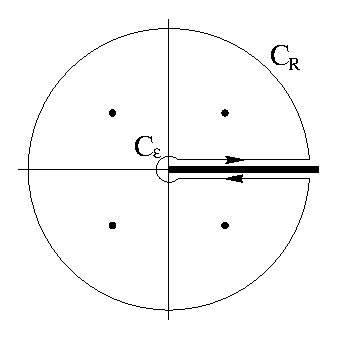
\includegraphics[width=0.25\textwidth]{fcv/residue/contepsrfourdot}
    \end{center}
    \caption{Possible path of integration.}
    \label{contepsrfourdot}
  \end{figure}

  Integrating on this contour would work because the value of the integrand
  below the branch cut is a constant times the value of the integrand above
  the branch cut.  After demonstrating that the integrals along $C_\epsilon$
  and $C_R$ vanish in the limits as $\epsilon \to 0$ and $R \to \infty$ we would
  see that the value of the integral is a constant times the sum of the residues
  at the four poles.  However, this is not the only, (and not the best), contour
  that can be used to evaluate the real integral.  Consider the value of
  the integral on the line $\arg(z) = \theta$.
  \[
  f( r \e^{\imath \theta} ) = \frac{ r^a \e^{\imath a \theta} }{ 1 + r^4 \e^{\imath 4 \theta} }
  \]
  If $\theta$ is a integer multiple of $\pi/2$ then the integrand is a
  constant multiple of
  \[
  f(x) = \frac{ r^a }{ 1 + r^4 }.
  \]
  Thus any of the contours in Figure~\ref{threechoice} can be used to
  evaluate the real integral.  The only difference is how many residues
  we have to calculate.  Thus we choose the first contour in
  Figure~\ref{threechoice}.
  We put a branch cut on the negative real axis
  and choose the branch $-\pi < \arg(z) < \pi$ to satisfy $f(1) = 1$.

  \begin{figure}[tb!]
    \begin{center}
      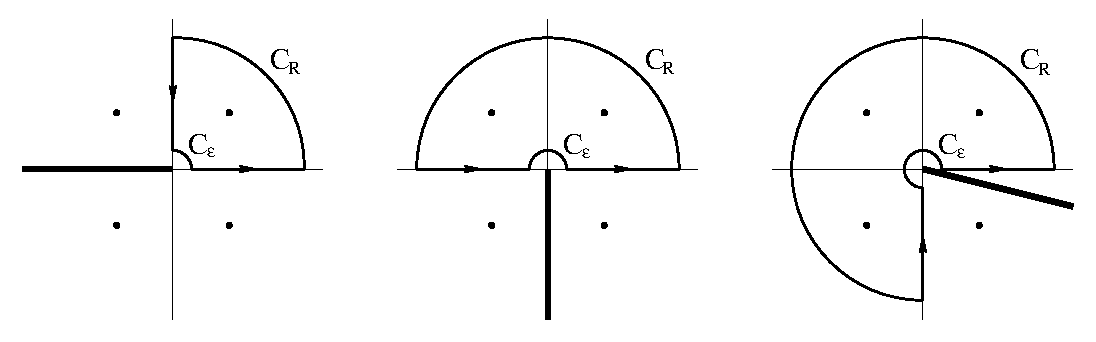
\includegraphics[width=\textwidth]{fcv/residue/threechoice}
    \end{center}
    \caption{Possible paths of integration.}
    \label{threechoice}
  \end{figure}

  We evaluate the integral along $C$ with the Residue Theorem.
  \[
  \int_C \frac{z^a}{1 + z^4} \,\dd z = \imath 2 \pi \Res \left( \frac{z^a}{1+z^4},
    z = \frac{1 + \imath}{\sqrt{2}} \right)
  \]
  Let $a = \alpha + \imath \beta$ and $z = r \e^{\imath \theta}$.  Note that
  \[
  |z^a| = | (r \e^{\imath \theta})^{\alpha + \imath \beta} | = r^{\alpha} \e^{- \beta \theta}.
  \]
  The integral on $C_\epsilon$ vanishes as $\epsilon \to 0$.  We demonstrate
  this with the maximum modulus integral bound.
  \begin{align*}
    \left| \int_{C_\epsilon} \frac{z^a}{1+z^4} \,\dd z \right|
    &\leq \frac{\pi \epsilon}{2} \max_{z \in C_\epsilon}
    \left| \frac{z^a}{1+z^4} \right| \\
    &\leq \frac{\pi \epsilon}{2} \frac{\epsilon^\alpha \e^{\pi |\beta|/2}}
    {1 - \epsilon^4} \\
    &\to 0 \quad \mathrm{as}\ \epsilon \to 0
  \end{align*}
  The integral on $C_R$ vanishes as $R \to \infty$.
  \begin{align*}
    \left| \int_{C_R} \frac{z^a}{1+z^4}\,\dd z \right|
    &\leq \frac{\pi R}{2} \max_{z \in C_R}
    \left| \frac{z^a}{1+z^4} \right| \\
    &\leq \frac{\pi R}{2} \frac{R^\alpha \e^{\pi |\beta| / 2}}
    { R^4 - 1 } \\
    &\to 0 \quad \mathrm{as}\ R \to \infty
  \end{align*}
  The value of the integrand on the positive imaginary axis,
  $z = x \e^{\imath \pi/2}$, is
  \[
  \frac{ (x \e^{\imath \pi/2} )^a }{ 1 + (x \e^{\imath \pi/2} )^4 }
  = \frac{ x^a \e^{\imath \pi a / 2} }{ 1 + x^4 }.
  \]
  We take the limit as $\epsilon \to 0$ and $R \to \infty$.
  \begin{gather*}
    \int_0^\infty \frac{x^a}{1 + x^4} \,\dd x
    + \int_\infty^0 \frac{ x^a \e^{\imath \pi a / 2} }{1 + x^4} \e^{\imath \pi/2} \,\dd x
    = \imath 2 \pi \Res \left( \frac{z^a}{1+z^4}, \e^{\imath \pi/4} \right) \\
    \left( 1 - \e^{\imath \pi (a+1) / 2} \right) \int_0^\infty \frac{x^a}{1 + x^4} \,\dd x
    = \imath 2 \pi \lim_{z \to \e^{\imath \pi/4} }
    \left( \frac{z^a (z - \e^{\imath \pi/2}) }{1+z^4} \right) \\
    \int_0^\infty \frac{x^a}{1 + x^4} \,\dd x
    = \frac{ \imath 2 \pi }{ 1 - \e^{\imath \pi (a+1) / 2} } \lim_{z \to \e^{\imath \pi/4} }
    \left( \frac{a z^a (z - \e^{\imath \pi/2}) + z^a }{4 z^3} \right) \\
    \int_0^\infty \frac{x^a}{1 + x^4} \,\dd x
    = \frac{\imath 2 \pi}{ 1 - \e^{\imath \pi (a+1) / 2} }  \frac{ \e^{\imath \pi a / 4} }{ 4 \e^{\imath 3 \pi / 4} } \\
    \int_0^\infty \frac{x^a}{1 + x^4} \,\dd x
    = \frac{ - \imath \pi }{ 2( \e^{ -\imath \pi (a+1) / 4} - \e^{ \imath \pi (a+1)/4} ) } \\
    \boxed{
      \int_0^\infty \frac{x^a}{1 + x^4} \,\dd x
      = \frac{\pi}{4} \csc \left( \frac{ \pi(a+1) }{ 4 } \right)
      }
  \end{gather*}
\end{Solution}


















%% \int_0^\infty \frac{x^{1/2} \log x}{(x+1)^2} \,\dd x 
\begin{Solution}
  \label{solution x^(1/2) log x / (x+1)^2}
  Consider the branch of $f(z) = z^{1/2} \log z / (z+1)^2$ with a 
  branch cut on the positive real axis and $0 < \arg z < 2 \pi$.  We integrate
  this function on the contour in Figure~\ref{contepsr}.

  We use the maximum modulus integral bound to show that the integral on 
  $C_\rho$ vanishes as $\rho \to 0$.
  \begin{align*}
    \left| \int_{C_\rho} \frac{ z^{1/2} \log z }{ (z+1)^2 } \,\dd z \right|
    &\leq 2 \pi \rho \max_{C_\rho} \left| 
      \frac{ z^{1/2} \log z }{ (z+1)^2 } \right| \\
    &= 2 \pi \rho \frac{\rho^{1/2} (2 \pi - \log \rho ) }
    { (1 - \rho)^2 } \\
    &\to 0\ \mathrm{as}\ \rho \to 0
  \end{align*}
  The integral on $C_R$ vanishes as $R \to \infty$.
  \begin{align*}
    \left| \int_{C_R} \frac{z^{1/2} \log z }{ (z+1)^2 } \,\dd z \right|
    &\leq 2 \pi R \max_{C_R} \left| 
      \frac{ z^{1/2} \log z }{ (z+1)^2 } \right| \\
    &= 2 \pi R \frac{ R^{1/2} (\log R + 2 \pi) }
    { (R-1)^2 } \\
    &\to 0\ \mathrm{as}\ R \to \infty
  \end{align*}

  Above the branch cut, ($z = x \e^{\imath 0}$), the integrand is,
  \[
  f(x \e^{\imath 0 }) = \frac{ x^{1/2} \log x }{ (x+1)^2 }.
  \]
  Below the branch cut, ($z = x \e^{\imath 2 \pi}$ ), we have,
  \[
  f(x \e^{\imath 2 \pi }) = \frac{ - x^{1/2} ( \log x + \imath \pi ) }{ (x+1)^2 }.
  \]
  Taking the limit as $\rho \to 0$ and $R \to \infty$, the residue theorem
  gives us
  \[
  \int_0^\infty \frac{ x^{1/2} \log x }{ (x+1)^2 } \,\dd x
  + \int_\infty^0 \frac{ - x^{1/2} ( \log x + \imath 2 \pi ) }{ (x+1)^2 } \,\dd x
  = \imath 2 \pi \Res \left( \frac{ z^{1/2} \log z }{ (z+1)^2 }, -1 \right).
  \]
  \[
  2 \int_0^\infty \frac{ x^{1/2} \log x }{ (x+1)^2 } \,\dd x
  + \imath 2 \pi \int_0^\infty \frac{ x^{1/2} }{ (x+1)^2 } \,\dd x
  = \imath 2 \pi \lim_{z \to -1} \frac{\dd}{\dd z} ( z^{1/2} \log z )
  \]
  \[
  2 \int_0^\infty \frac{ x^{1/2} \log x }{ (x+1)^2 } \,\dd x
  + \imath 2 \pi \int_0^\infty \frac{ x^{1/2} }{ (x+1)^2 } \,\dd x
  = \imath 2 \pi \lim_{z \to -1} \left( \frac{1}{2} z^{-1/2} \log z 
    + z^{1/2} \frac{1}{z} \right)
  \]
  \[
  2 \int_0^\infty \frac{ x^{1/2} \log x }{ (x+1)^2 } \,\dd x
  + \imath 2 \pi \int_0^\infty \frac{ x^{1/2} }{ (x+1)^2 } \,\dd x
  = \imath 2 \pi \left( \frac{1}{2} (-\imath) (\imath \pi)  - \imath \right)
  \]
  \[
  2 \int_0^\infty \frac{ x^{1/2} \log x }{ (x+1)^2 } \,\dd x
  + \imath 2 \pi \int_0^\infty \frac{ x^{1/2} }{ (x+1)^2 } \,\dd x
  = 2 \pi + \imath \pi^2
  \]
  Equating real and imaginary parts,
  \[
  \boxed{
    \int_0^\infty \frac{ x^{1/2} \log x }{ (x+1)^2 }\,\dd x = \pi, \qquad
    \int_0^\infty \frac{ x^{1/2} }{ (x+1)^2 }\,\dd x = \frac{\pi}{2}.
    }
  \]
\end{Solution}











%%-----------------------------------------------------------------------------
\begin{large}
  \noindent
  \textbf{Exploiting Symmetry}
\end{large}










%% I(a) = \pv\int_{-\infty}^\infty \frac{ \e^{a x} }{ \e^x - \e^{-x} } \,\dd x
\begin{Solution}
  \label{solution e ax / (e x - e -x)}
  \textbf{Convergence.}
  The integrand, 
  \[
  \frac{ \e^{a z} }{ \e^z - \e^{-z} } = \frac{ \e^{a z} }{ 2 \sinh( z ) },
  \]
  has first order poles at $z = \imath n \pi$, $n \in \mathbb{Z}$.  To study 
  convergence, we split the domain of integration.
  \[
  \int_{-\infty}^\infty = \int_{-\infty}^{-1} + \int_{-1}^1 + \int_1^\infty
  \]
  The principal value integral
  \[
  \pv\int_{-1}^1 \frac{ \e^{a x} }{ \e^x - \e^{-x} } \,\dd x
  \]
  exists for any $a$ because the integrand has only a first order pole 
  on the path of integration.

  Now consider the integral on $(1 \ldots \infty)$.
  \begin{align*}
    \left| \int_1^\infty \frac{ \e^{a x} }{ \e^x - \e^{-x} } \,\dd x \right|
    &= \int_1^\infty \frac{ \e^{(a-1) x} }{ 1 - \e^{-2x} } \,\dd x \\
    &\leq \frac{1}{1 - \e^{-2} } \int_1^\infty \e^{(a-1) x} \,\dd x
  \end{align*}
  This integral converges for $a-1 < 0$; $a < 1$.

  Finally consider the integral on $(-\infty \ldots -1)$.
  \begin{align*}
    \left| \int_{-\infty}^{-1} \frac{ \e^{a x} }{ \e^x - \e^{-x} } \,\dd x \right|
    &= \int_{-\infty}^{-1} \frac{ \e^{(a+1) x} }{ 1 - \e^{2x} } \,\dd x \\
    &\leq \frac{1}{1 - \e^{-2} } \int_{-\infty}^{-1} \e^{(a+1) x} \,\dd x
  \end{align*}
  This integral converges for $a+1 > 0$; $a > -1$.

  Thus we see that the integral for $I(a)$ converges for real $a$, $|a| < 1$.


  \textbf{Choice of Contour.}
  Consider the contour $C$ that is the boundary of the region:
  $-R < x < R$, $0 < y < \pi$.  The integrand has no singularities inside
  the contour.  There are first order poles on the contour at $z = 0$
  and $z = \imath \pi$.  The value of the integral along the contour is 
  $\imath \pi$ times the sum of these two residues.

  The integrals along the vertical sides of the contour vanish as 
  $R \to \infty$.
  \begin{align*}
    \left| \int_{R}^{R + \imath \pi} \frac{ \e^{a z} }{ \e^z - \e^{-z} } \,\dd z \right|
    &\leq \pi \max_{z \in (R \ldots R + \imath \pi)}
    \left| \frac{ \e^{a z} }{ \e^z - \e^{-z} } \right| \\
    &\leq \pi \frac{ \e^{a R} }{ \e^R - \e^{-R} } \\
    &\to 0\ \mathrm{as}\ R \to \infty
  \end{align*}
  \begin{align*}
    \left| \int_{-R}^{-R + \imath \pi} \frac{ \e^{a z} }{ \e^z - \e^{-z} } \,\dd z \right|
    &\leq \pi \max_{z \in (-R \ldots -R + \imath \pi)}
    \left| \frac{ \e^{a z} }{ \e^z - \e^{-z} } \right| \\
    &\leq \pi \frac{ \e^{-a R} }{ \e^{-R} - \e^R } \\
    &\to 0\ \mathrm{as}\ R \to \infty
  \end{align*}


  \textbf{Evaluating the Integral.}
  We take the limit as $R \to \infty$ and apply the residue theorem.
  \begin{multline*}
    \int_{-\infty}^\infty \frac{ \e^{a x} }{ \e^x - \e^{-x} } \,\dd x
    + \int_{\infty + \imath \pi}^{-\infty + \imath \pi} 
    \frac{ \e^{a z} }{ \e^z - \e^{-z} } \,\dd z \\
    = \imath \pi \Res \left( \frac{ \e^{a z} }{ \e^z - \e^{-z} }, z = 0 \right)
    + \imath \pi \Res \left( \frac{ \e^{a z} }{ \e^z - \e^{-z} }, 
      z = \imath \pi \right) 
  \end{multline*}
  \begin{gather*}
    \int_{-\infty}^\infty \frac{ \e^{a x} }{ \e^x - \e^{-x} } \,\dd x
    + \int_\infty^{-\infty} 
    \frac{ \e^{a (x + \imath \pi} }{ \e^{x + \imath \pi} - \e^{-x - \imath \pi} } \,\dd z
    = \imath \pi \lim_{z \to 0} \frac{ z \e^{a z} }{ 2 \sinh(z) }
    + \imath \pi \lim_{z \to \imath \pi} 
    \frac{ (z - \imath \pi) \e^{a z} }{ 2 \sinh(z) } \\
    (1 + \e^{\imath a \pi} )\int_{-\infty}^\infty \frac{ \e^{a x} }{ \e^x - \e^{-x} } \,\dd x
    = \imath \pi \lim_{z \to 0} \frac{ \e^{a z} + a z \e^{a z} }{ 2 \cosh(z) }
    + \imath \pi \lim_{z \to \imath \pi} 
    \frac{ \e^{a z} + a (z - \imath \pi) \e^{a z} }{ 2 \cosh(z) } \\
    (1 + \e^{\imath a \pi} )\int_{-\infty}^\infty \frac{ \e^{a x} }{ \e^x - \e^{-x} } \,\dd x
    = \imath \pi \frac{ 1 }{ 2 }
    + \imath \pi \frac{ \e^{\imath a \pi} }{ - 2 } \\
    \int_{-\infty}^\infty \frac{ \e^{a x} }{ \e^x - \e^{-x} } \,\dd x
    = \frac{ \imath \pi (1 - \e^{\imath a \pi}) }{ 2 (1 + \e^{\imath a \pi}) } \\
    \int_{-\infty}^\infty \frac{ \e^{a x} }{ \e^x - \e^{-x} } \,\dd x
    = \frac{\pi}{2} \frac{ \imath (\e^{-\imath a \pi / 2} - \e^{\imath a \pi / 2}) }
    { \e^{\imath a \pi / 2} + \e^{\imath a \pi / 2} } \\
    \boxed{
      \int_{-\infty}^\infty \frac{ \e^{a x} }{ \e^x - \e^{-x} } \,\dd x
      = \frac{\pi}{2} \tan \left( \frac{a \pi}{2} \right)
      }
  \end{gather*}
\end{Solution}












%% \int_0^\infty \frac{\dd x}{x^3+1}.
\begin{Solution}
  \label{solution 1/(x^3+1)}
  \begin{enumerate}
    %%
    %%
    %%
  \item
    \[
    \int_0^\infty \frac{\dd x}{ \left(1 + x^2 \right)^2 }
    = \frac{1}{2} \int_{-\infty}^\infty \frac{\dd x}{ \left(1 + x^2 \right)^2 }
    \]
    We apply Result~\ref{result int mii f(x)} to the integral on the real axis.
    First we verify that the integrand vanishes fast enough in the upper half 
    plane.
    \[
    \lim_{R \to \infty} \left( R \max_{z \in C_R} \left| \frac{1}{ \left( 1 + z^2 \right)^2 }
      \right| \right) 
    = \lim_{R \to \infty} \left( R \frac{1}{ \left( R^2 - 1 \right)^2 } \right)
    = 0
    \]
    Then we evaluate the integral with the residue theorem.
    \begin{align*}
      \int_{-\infty}^\infty \frac{\dd x}{ \left(1 + x^2 \right)^2 }
      &= \imath 2 \pi \Res \left( \frac{1}{ \left( 1 + z^2 \right)^2 }, z = \imath \right) \\
      &= \imath 2 \pi \Res \left( \frac{1}{ (z - \imath)^2 (z + \imath)^2 }, z = \imath \right) \\
      &= \imath 2 \pi \lim_{z \to \imath} \frac{\dd}{\dd z} \frac{1}{(z + \imath)^2} \\
      &= \imath 2 \pi \lim_{z \to \imath} \frac{-2}{(z + \imath)^3} \\
      &= \frac{\pi}{2}
    \end{align*}
    \[
    \boxed{
      \int_0^\infty \frac{\dd x}{ \left(1 + x^2 \right)^2 } = \frac{\pi}{4}
      }
    \]
    %%
    %%
    %%
  \item
    We wish to evaluate
    \[
    \int_0^\infty \frac{\dd x}{x^3 + 1}.
    \]
    Let the contour $C$ be the boundary of the region 
    $0 < r < R$, $0 < \theta < 2 \pi / 3$.
    We factor the denominator of the integrand to see that the contour 
    encloses the simple pole at $\e^{\imath \pi / 3}$ for $R > 1$.
    \[
    z^3 + 1 = (z - \e^{\imath \pi / 3}) (z + 1) (z - \e^{- \imath \pi / 3})
    \]
    We calculate the residue at that point.
    \begin{align*}
      \Res \left( \frac{1}{z^3 + 1}, z = \e^{\imath \pi / 3} \right)
      &= \lim_{z \to \e^{\imath \pi/3}} \left( (z - \e^{\imath \pi/3}) \frac{1}{z^3 + 1} \right) 
      \\
      &= \lim_{z \to \e^{\imath \pi/3}} \left( \frac{1}{(z + 1) (z- \e^{- \imath \pi / 3})} \right)
      \\
      &= \frac{1}{(\e^{\imath \pi/3} + 1) (\e^{\imath \pi/3} - \e^{- \imath \pi / 3})}
      \\
      &= - \frac{ \e^{\imath \pi/3} }{ 3 }
    \end{align*}
    We use the residue theorem to evaluate the integral.
    \[
    \oint_C \frac{\dd z}{z^3 + 1} = - \frac{ \imath 2 \pi \e^{\imath \pi/3} }{ 3 }
    \]

    Let $C_R$ be the circular arc portion of the contour.
    \begin{align*}
      \int_C \frac{\dd z}{z^3 + 1} 
      &= \int_0^R \frac{\dd x}{x^3 + 1} 
      + \int_{C_R} \frac{\dd z}{z^3 + 1} -
      \int_0^R \frac{\e^{\imath 2 \pi/3}\,\dd x}{x^3 + 1}  
      \\
      &= (1 + \e^{- \imath \pi / 3}) \int_0^R \frac{\dd x}{x^3 + 1}
      + \int_{C_R} \frac{\dd z}{z^3 + 1}
    \end{align*}

    We show that the integral along $C_R$ vanishes as $R \to \infty$ with the maximum
    modulus integral bound.
    \[
    \left| \int_{C_R} \frac{\dd z}{z^3 + 1} \right| 
    \leq \frac{2 \pi R}{3} \frac{1}{R^3 - 1} 
    \to 0 \quad \mathrm{as}\ R \to \infty
    \]
    We take $R \to \infty$ and solve for the desired integral.
    \begin{gather*}
      \left( 1 + \e^{-\imath \pi/3} \right) \int_0^\infty \frac{\dd x}{x^3 + 1} 
      = - \frac{ \imath 2 \pi \e^{\imath \pi/3} }{ 3 }
      \\
      \int_0^\infty \frac{\dd x}{x^3 + 1} = \frac{2 \pi}{3 \sqrt{3}}
    \end{gather*}
  \end{enumerate}
\end{Solution}










%% \int_0^\infty \frac{\dd x}{1 + x^6}
\begin{Solution}
  \label{solution 1/(1+x^6)}
  \textbf{Method 1: Semi-Circle Contour.}
  We wish to evaluate the integral
  \[
  I = \int_0^\infty \frac{\dd x}{1 + x^6}.
  \]
  We note that the integrand is an even function and express $I$ as an integral
  over the whole real axis.
  \[
  I = \frac{1}{2} \int_{-\infty}^\infty \frac{\dd x}{1 + x^6}
  \]
  Now we will evaluate the integral using contour integration.
  We close the path of integration in the upper half plane.
  Let $\Gamma_R$ be the semicircular arc from $R$ to $-R$ in the upper half plane.
  Let $\Gamma$ be the union of $\Gamma_R$ and the interval $[-R,R]$.
  (See Figure~\ref{semi_circle_1x6}.)
  \begin{figure}[tb!]
    \begin{center}
      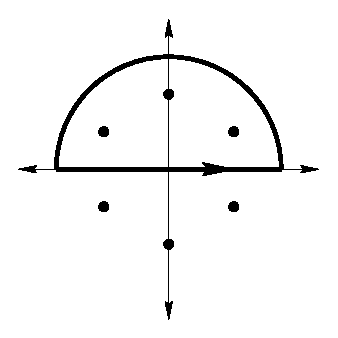
\includegraphics[width=0.25\textwidth]{fcv/residue/semi_circle_1x6}
    \end{center}
    \caption{The semi-circle contour.}
    \label{semi_circle_1x6}
  \end{figure}

  We can evaluate the integral along $\Gamma$ with the residue theorem.
  The integrand has first order poles at $z = \e^{\imath \pi (1 + 2 k) / 6}$, 
  $k = 0,1,2,3,4,5$.  Three of these poles are in the upper half plane.
  For  $R > 1$, we have
  \begin{align*}
    \int_\Gamma \frac{1}{z^6+1} \,\dd z
    &= \imath 2 \pi \sum_{k = 0}^2 
    \Res\left( \frac{1}{z^6+1}, \e^{\imath \pi (1 + 2 k) / 6} \right) \\
    &= \imath 2 \pi \sum_{k = 0}^2 
    \lim_{z \to \e^{\imath \pi (1 + 2 k) / 6} } 
    \frac{z - \e^{\imath \pi (1 + 2 k) / 6}}{z^6+1} \\
    \intertext{Since the numerator and denominator vanish, we apply 
      L'Hospital's rule.}
    &= \imath 2 \pi \sum_{k = 0}^2 
    \lim_{z \to \e^{\imath \pi (1 + 2 k) / 6} } \frac{1}{6 z^5} \\
    &= \frac{\imath \pi}{3} \sum_{k = 0}^2 \e^{- \imath \pi 5 (1 + 2 k) / 6} \\
    &= \frac{\imath \pi}{3} \left( \e^{- \imath \pi 5 / 6}
      + \e^{- \imath \pi 15 / 6} + \e^{- \imath \pi 25 / 6} \right) \\
    &= \frac{\imath \pi}{3} \left( \e^{- \imath \pi 5 / 6}
      + \e^{- \imath \pi / 2} + \e^{- \imath \pi / 6} \right) \\
    &= \frac{\imath \pi}{3} \left( \frac{-\sqrt{3} - \imath}{2}
      - \imath + \frac{\sqrt{3} - \imath}{2} \right) \\
    &= \frac{2 \pi}{3}
  \end{align*}
  Now we examine the integral along $\Gamma_R$.
  We use the maximum modulus integral bound to show that the value of the 
  integral vanishes as $R \to \infty$.
  \begin{align*}
    \left| \int_{\Gamma_R} \frac{1}{z^6+1} \,\dd z \right|
    &\leq \pi R \max_{z \in \Gamma_R} \left| \frac{1}{z^6+1} \right| \\
    &= \pi R \frac{1}{R^6-1} \\
    &\to 0 \quad \mathrm{as}\ R \to \infty.
  \end{align*}
  Now we are prepared to evaluate the original real integral.
  \begin{gather*}
    \int_\Gamma \frac{1}{z^6+1} \,\dd z = \frac{2 \pi}{3} \\
    \int_{-R}^R \frac{1}{x^6 + 1} \,\dd x +
    \int_{\Gamma_R} \frac{1}{z^6+1} \,\dd z = \frac{2 \pi}{3} \\
    \intertext{We take the limit as $R \to \infty$.}
    \int_{-\infty}^\infty \frac{1}{x^6 + 1} \,\dd x = \frac{2 \pi}{3} \\
    \int_0^\infty \frac{1}{x^6 + 1} \,\dd x = \frac{\pi}{3} 
  \end{gather*}
  We would get the same result by closing the path of integration in
  the lower half plane.  Note that in this case the closed contour would
  be in the negative direction.


  \textbf{Method 2: Wedge Contour.}
  Consider the contour $\Gamma$, which starts at the origin, goes to the point
  $R$ along the real axis, then to the point $R \e^{\imath \pi / 3}$ along
  a circle of radius $R$ and then back to the origin along the ray
  $\theta = \pi / 3$.  (See Figure~\ref{wedge_1x6}.)
  \begin{figure}[tb!]
    \begin{center}
      \includegraphics[width=0.25\textwidth]{fcv/residue/wedge_1x6}
    \end{center}
    \caption{The wedge contour.}
    \label{wedge_1x6}
  \end{figure}

  We can evaluate the integral along $\Gamma$ with the residue theorem.
  The integrand has one first order pole inside the contour at 
  $z = \e^{\imath \pi / 6}$.   For  $R > 1$, we have
  \begin{align*}
    \int_\Gamma \frac{1}{z^6+1} \,\dd z
    &= \imath 2 \pi \Res\left( \frac{1}{z^6+1}, \e^{\imath \pi / 6} \right) \\
    &= \imath 2 \pi \lim_{z \to \e^{\imath \pi / 6} } 
    \frac{z - \e^{\imath \pi / 6}}{z^6+1} \\
    \intertext{Since the numerator and denominator vanish, we apply 
      L'Hospital's rule.}
    &= \imath 2 \pi \lim_{z \to \e^{\imath \pi / 6} } \frac{1}{6 z^5} \\
    &= \frac{\imath \pi}{3} \e^{- \imath \pi 5 / 6} \\
    &= \frac{\pi}{3} \e^{- \imath \pi / 3} 
    %%        &= \frac{\imath \pi}{3} \frac{-\sqrt{3} - \imath}{2} \\
    %%       &= \frac{\pi}{6} (1 - \imath \sqrt{3})
  \end{align*}
  Now we examine the integral along the circular arc, $\Gamma_R$.
  We use the maximum modulus integral bound to show that the value of the 
  integral vanishes as $R \to \infty$.
  \begin{align*}
    \left| \int_{\Gamma_R} \frac{1}{z^6+1} \,\dd z \right|
    &\leq \frac{\pi R}{3} \max_{z \in \Gamma_R} 
    \left| \frac{1}{z^6+1} \right| \\
    &= \frac{\pi R}{3} \frac{1}{R^6-1} \\
    &\to 0 \quad \mathrm{as}\ R \to \infty.
  \end{align*}
  Now we are prepared to evaluate the original real integral.
  \begin{gather*}
    \int_\Gamma \frac{1}{z^6+1} \,\dd z = \frac{\pi}{3} \e^{- \imath \pi / 3} \\
    \int_0^R \frac{1}{x^6 + 1} \,\dd x
    + \int_{\Gamma_R} \frac{1}{z^6 + 1}\,\dd  z
    + \int_{R \e^{\imath \pi / 3}}^0 \frac{1}{z^6 + 1}\,\dd  z
    = \frac{\pi}{3} \e^{- \imath \pi / 3} \\
    \int_0^R \frac{1}{x^6 + 1} \,\dd x
    + \int_{\Gamma_R} \frac{1}{z^6 + 1}\,\dd  z
    + \int_R^0 \frac{1}{x^6 + 1} \e^{\imath \pi / 3} \,\dd x
    = \frac{\pi}{3} \e^{- \imath \pi / 3} \\
    \intertext{We take the limit as $R \to \infty$.}
    \left( 1 - \e^{\imath \pi / 3} \right) \int_0^\infty \frac{1}{x^6 + 1} \,\dd x
    = \frac{\pi}{3} \e^{- \imath \pi / 3} \\
    \int_0^\infty \frac{1}{x^6 + 1} \,\dd x 
    = \frac{\pi}{3} \frac{ \e^{- \imath \pi / 3} }{ 1 - \e^{\imath \pi / 3} } \\
    \int_0^\infty \frac{1}{x^6 + 1} \,\dd x 
    = \frac{\pi}{3} \frac{ (1 - \imath \sqrt{3})/2 }{ 1 - (1 + \imath \sqrt{3})/2 }\\
    \int_0^\infty \frac{1}{x^6 + 1} \,\dd x = \frac{\pi}{3} 
  \end{gather*}
\end{Solution}









%% \int_0^\infty \cos(x^2)\,\dd x 
\begin{Solution}
  \label{solution cos x^2}
  First note that 
  \[
  \cos(2 \theta) \geq 1 - \frac{4}{\pi} \theta, 
  \quad 0 \leq \theta \leq \frac{\pi}{4}.
  \]
  These two functions are plotted in Figure~\ref{bndcos2t}.
  To prove this inequality analytically, note that the two functions are 
  equal at the endpoints of the interval and that $\cos(2 \theta)$ is concave 
  downward on the interval,
  \[
  \frac{\dd^2}{\dd \theta^2} \cos(2 \theta) = - 4 \cos(2 \theta) \leq 0 \quad 
  \mathrm{for}\ 0 \leq \theta \leq \frac{\pi}{4},
  \]
  while $1 - 4 \theta / \pi$ is linear.

  \begin{figure}[tb!]
    \begin{center}
      \includegraphics[width=0.3\textwidth]{fcv/residue/bndcos2t}
    \end{center}
    \caption{The two functions.}
    \label{bndcos2t}
  \end{figure}

  Let $C_R$ be the quarter circle of radius $R$ from $\theta = 0$ to 
  $\theta = \pi/4$.  The integral along this contour vanishes as 
  $R \to \infty$.
  \begin{align*}
    \left| \int_{C_R} \e^{-z^2}\,\dd z \right|
    &\leq \int_0^{\pi/4} \left| \e^{-(R \e^{\imath \theta})^2} \right| 
    \left| R \imath \e^{\imath \theta} \right| \,\dd \theta \\
    &\leq \int_0^{\pi/4} R \e^{-R^2 \cos(2 \theta)} \,\dd \theta \\
    &\leq \int_0^{\pi/4} R \e^{-R^2 (1 - 4 \theta / \pi)} \,\dd \theta \\
    &= \left[ R  \frac{\pi}{4 R^2} \e^{-R^2 (1 - 4 \theta / \pi)} 
    \right]_0^{\pi/4} \\
    &= \frac{\pi}{4 R} \left( 1 - \e^{-R^2} \right) \\
    &\to 0\ \mathrm{as}\ R \to \infty
  \end{align*}
  Let $C$ be the boundary of the domain $0 < r < R$, $0 < \theta < \pi / 4$.
  Since the integrand is analytic inside $C$ the integral along $C$ is 
  zero.  Taking the limit as $R \to \infty$, the integral from $r = 0$ to $\infty$
  along $\theta = 0$ is equal to the integral from $r = 0$ to $\infty$
  along $\theta = \pi / 4$.
  \[
  \int_0^\infty \e^{-x^2}\,\dd x 
  = \int_0^\infty \e^{- \left(\frac{1 + \imath}{\sqrt{2}} x \right)^2 }
  \frac{1 + \imath}{\sqrt{2}} \,\dd x
  \]
  \[
  \int_0^\infty \e^{-x^2}\,\dd x 
  = \frac{1 + \imath}{\sqrt{2}} \int_0^\infty \e^{- \imath x^2 } \,\dd x
  \]
  \[
  \int_0^\infty \e^{-x^2}\,\dd x 
  = \frac{1 + \imath}{\sqrt{2}} \int_0^\infty \left( \cos(x^2) - \imath \sin(x^2) 
  \right)\,\dd x
  \]
  \[
  \int_0^\infty \e^{-x^2}\,\dd x 
  = \frac{1}{\sqrt{2}} 
  \left( \int_0^\infty \cos(x^2)\,\dd x + \int_0^\infty \sin(x^2)\,\dd x \right)
  + \frac{\imath}{\sqrt{2}}
  \left( \int_0^\infty \cos(x^2)\,\dd x - \int_0^\infty \sin(x^2)\,\dd x \right)
  \]
  We equate the imaginary part of this equation to see that the integrals 
  of $\cos(x^2)$ and $\sin(x^2)$ are equal.
  \[
  \int_0^\infty \cos(x^2)\,\dd x = \int_0^\infty \sin(x^2)\,\dd x
  \]
  The real part of the equation then gives us the desired identity.
  \[
  \boxed{
    \int_0^\infty \cos(x^2)\,\dd x = \int_0^\infty \sin(x^2)\,\dd x = \frac{1}{\sqrt{2}}
    \int_0^\infty \e^{-x^2}\,\dd x
    }
  \]
\end{Solution}



















%% $\frac{x}{\sinh x}$
\begin{Solution}
  \label{solution x/sinh x}
  Consider the box contour $C$ that is the boundary of the rectangle
  $-R \leq x \leq R$, $0 \leq y \leq \pi$.   There is a removable singularity
  at $z = 0$ and a first order pole at $z = \imath \pi$.  By the residue theorem,
  \begin{align*}
    \pv\int_C \frac{z}{\sinh z} \,\dd z
    &= \imath \pi \Res \left( \frac{z}{\sinh z}, \imath \pi \right) \\
    &= \imath \pi \lim_{z \to \imath \pi} \frac{ z (z - \imath \pi) }{ \sinh z } \\
    &= \imath \pi \lim_{z \to \imath \pi} \frac{ 2 z - \imath \pi }{ \cosh z } \\
    &= \pi^2
  \end{align*}
  The integrals along the side of the box vanish as $R \to \infty$.
  \begin{align*}
    \left| \int_{\pm R}^{\pm R + \imath \pi} \frac{z}{\sinh z} \,\dd z \right|
    &\leq \pi \max_{z \in [\pm R, \pm R + \imath \pi]}
    \left| \frac{z}{\sinh z} \right| \\
    &\leq \pi \frac{R + \pi}{ \sinh R } \\
    &\to 0\ \mathrm{as}\ R \to \infty
  \end{align*}
  The value of the integrand on the top of the box is
  \[
  \frac{x + \imath \pi}{\sinh(x + \imath \pi)} = - \frac{x + \imath \pi}{ \sinh x }.
  \]
  Taking the limit as $R \to \infty$,
  \[
  \int_{-\infty}^\infty \frac{x}{\sinh x} \,\dd x
  + \pv\int_{-\infty}^\infty - \frac{x + \imath \pi}{\sinh x} \,\dd x
  = \pi^2.
  \]
  Note that 
  \[
  \pv\int_{-\infty}^\infty \frac{1}{\sinh x} \,\dd x = 0
  \]
  as there is a first order pole at $x = 0$ and the integrand is odd.
  \[
  \boxed{
    \int_{-\infty}^\infty \frac{x}{\sinh x} \,\dd x = \frac{\pi^2}{2}
    }
  \]
\end{Solution}



%% \int_{-\infty}^\infty \frac{\e^{a x}}{\e^x + 1} \,\dd x = \frac{\pi}{\sin(\pi a)}
\begin{Solution}
  \label{solution e ax / (e x + 1)}
  First we evaluate
  \[
  \int_{-\infty}^\infty \frac{\e^{a x}}{\e^x + 1}\,\dd x.
  \]
  Consider the rectangular contour in the positive direction with corners
  at $\pm R$ and $\pm R + \imath 2 \pi$.  With the maximum modulus integral bound
  we see that the integrals on the vertical sides of the contour vanish as 
  $R \to \infty$.
  \begin{gather*}
    \left| \int_R^{R + \imath 2 \pi} \frac{\e^{a z}}{\e^z + 1}\,\dd z \right|
    \leq 2 \pi \frac{\e^{a R}}{\e^R - 1} \to 0\ \mathrm{as}\ R \to \infty \\
    \left| \int_{-R + \imath 2 \pi}^{-R} \frac{\e^{a z}}{\e^z + 1}\,\dd z \right|
    \leq 2 \pi \frac{\e^{-a R}}{1 - \e^{-R}} \to 0\ \mathrm{as}\ R \to \infty
  \end{gather*}
  In the limit as $R$ tends to infinity, the integral on the rectangular
  contour is the sum of the integrals along the top and bottom sides.
  \begin{gather*}
    \int_C \frac{\e^{a z}}{\e^z + 1} \,\dd z = 
    \int_{-\infty}^\infty \frac{\e^{a x}}{\e^x + 1}\,\dd x
    + \int_\infty^{-\infty} \frac{\e^{a (x + \imath 2 \pi)}}{\e^{x + \imath 2 \pi} + 1}\,\dd x \\
    \int_C \frac{\e^{a z}}{\e^z + 1} \,\dd z = 
    (1 - \e^{- \imath 2 a \pi}) \int_{-\infty}^\infty \frac{\e^{a x}}{\e^x + 1}\,\dd x
  \end{gather*}
  The only singularity of the integrand inside the contour is a first order
  pole at $z = \imath \pi$.  We use the residue theorem to evaluate the 
  integral.
  \begin{align*}
    \int_C \frac{\e^{a z}}{\e^z + 1} \,\dd z 
    &= \imath 2 \pi \Res \left( \frac{\e^{a z}}{\e^z + 1}, \imath \pi \right) \\
    &= \imath 2 \pi \lim_{z \to \imath \pi} \frac{(z - \imath \pi) \e^{a z}}{\e^z+1} \\
    &= \imath 2 \pi \lim_{z \to \imath \pi} 
    \frac{a (z - \imath \pi) \e^{a z} + \e^{a z}}{\e^z} \\
    &= - \imath 2 \pi \e^{\imath a \pi}
  \end{align*}
  We equate the two results for the value of the contour integral.
  \begin{gather*}
    (1 - \e^{- \imath 2 a \pi}) \int_{-\infty}^\infty \frac{\e^{a x}}{\e^x + 1} \,\dd x = - \imath 2 \pi \e^{\imath a \pi} \\
    \int_{-\infty}^\infty \frac{\e^{a x}}{\e^x + 1} \,\dd x = \frac{\imath 2 \pi}{\e^{\imath a \pi} - \e^{- \imath a \pi}} \\
    \boxed{
      \int_{-\infty}^\infty \frac{\e^{a x}}{\e^x + 1} \,\dd x = \frac{\pi}{\sin(\pi a)}
      }
  \end{gather*}

  Now we derive the value of,
  \[
  \int_{-\infty}^\infty \frac{\cosh(b x)}{\cosh x} \,\dd x.
  \]
  First make the change of variables $x \to 2 x$ in the previous result.
  \begin{gather*}
    \int_{-\infty}^\infty \frac{\e^{2 a x}}{\e^{2 x} + 1} 2 \,\dd x = \frac{\pi}{\sin(\pi a)} \\
    \int_{-\infty}^\infty \frac{\e^{(2 a - 1) x}}{\e^x + \e^{-x}}\,\dd x = \frac{\pi}{\sin(\pi a)}
  \end{gather*}
  Now we set $b = 2 a - 1$.
  \[
  \int_{-\infty}^\infty \frac{\e^{b x}}{\cosh x}\,\dd x = \frac{\pi}{\sin(\pi (b+1)/2)}
  = \frac{\pi}{\cos(\pi b/2)} \quad \mathrm{for}\ -1 < b < 1
  \]
  Since the cosine is an even function, we also have,
  \[
  \int_{-\infty}^\infty \frac{\e^{-b x}}{\cosh x}\,\dd x 
  = \frac{\pi}{\cos(\pi b/2)} \quad \mathrm{for}\ -1 < b < 1
  \]
  Adding these two equations and dividing by 2 yields the desired result.
  \[
  \boxed{
    \int_{-\infty}^\infty \frac{\cosh(b x)}{\cosh x} \,\dd x
    = \frac{\pi}{\cos(\pi b/2)} \quad \mathrm{for}\ -1 < b < 1
    }
  \]
\end{Solution}










%% F(a,b) = \int_0^\pi \frac{ d \theta }{ (a + b \cos \theta)^2 }
\begin{Solution}
  \label{solution 1/(a + b cos theta)^2}
  \textbf{Real-Valued Parameters.}
  For $b = 0$, the integral has the value: $\pi / a^2$.  If $b$ is nonzero,
  then we can write the integral as
  \[
  F(a,b) = \frac{1}{b^2} \int_0^\pi \frac{ \dd \theta }{ (a/b + \cos \theta)^2 }.
  \]
  We define the new parameter $c = a/b$ and the function,
  \[
  G(c) = b^2 F(a,b)
  = \int_0^\pi \frac{ \dd \theta }{ (c + \cos \theta)^2 }.
  \]
  If $-1 \leq c \leq 1$ then the integrand has a double pole on the path 
  of integration.  The integral diverges.  Otherwise the integral exists.
  To evaluate the integral, we extend the range of integration to $(0..2 \pi)$
  and make the change of variables, $z = \e^{\imath \theta}$ to integrate along 
  the unit circle in the complex plane. 
  \[
  G(c) = \frac{1}{2} \int_0^{2 \pi} \frac{ \dd \theta }{ (c + \cos \theta)^2 }
  \]
  For this change of variables, we have,
  \[
  \cos \theta = \frac{z + z^{-1}}{2}, \qquad \dd \theta = \frac{\dd z}{\imath z}.
  \]
  \begin{align*}
    G(c)    &=  \frac{1}{2} \int_C \frac{ \dd z / (\imath z) }
    { (c + (z + z^{-1}) / 2)^2 } \\
    &=  - \imath 2 \int_C \frac{ z }
    { (2 c z + z^2 + 1)^2 } \,\dd z \\
    &=  - \imath 2 \int_C \frac{ z }
    { (z + c + \sqrt{c^2 - 1})^2 (z + c - \sqrt{c^2 - 1})^2 } 
    \,\dd z 
  \end{align*}

  If $c > 1$, then $-c - \sqrt{c^2 - 1}$ is outside the unit circle and 
  $-c + \sqrt{c^2 - 1}$ is inside the unit circle.  The integrand 
  has a second order pole inside the path of integration.  We evaluate the 
  integral with the residue theorem.
  \begin{align*}
    G(c)    &= - \imath 2 \imath 2 \pi \Res \left(
      \frac{ z }{ (z + c + \sqrt{c^2 - 1})^2 (z + c - \sqrt{c^2 - 1})^2 },
      z = -c + \sqrt{c^2 - 1} \right) \\
    &= 4 \pi \lim_{ z \to -c + \sqrt{c^2 - 1} } 
    \frac{\dd}{\dd z} \frac{ z }{ (z + c + \sqrt{c^2 - 1})^2 } \\
    &= 4 \pi \lim_{ z \to -c + \sqrt{c^2 - 1} } \left(
      \frac{ 1 }{ (z + c + \sqrt{c^2 - 1})^2 } 
      - \frac{ 2 z }{ (z + c + \sqrt{c^2 - 1})^3 } \right) \\
    &= 4 \pi \lim_{ z \to -c + \sqrt{c^2 - 1} } 
    \frac{ c + \sqrt{c^2-1} - z }{ (z + c + \sqrt{c^2 - 1})^3 } \\
    &= 4 \pi \frac{ 2 c }{ (2 \sqrt{c^2 - 1})^3 } \\
    &= \frac{ \pi c }{ \sqrt{(c^2 - 1)^3} } 
  \end{align*}

  If $c < 1$, then $-c - \sqrt{c^2 - 1}$ is inside the unit circle and 
  $-c + \sqrt{c^2 - 1}$ is outside the unit circle.  
  \begin{align*}
    G(c)    &= -\imath 2 \imath 2 \pi \Res \left(
      \frac{ z }{ (z + c + \sqrt{c^2 - 1})^2 (z + c - \sqrt{c^2 - 1})^2 },
      z = -c - \sqrt{c^2 - 1} \right) \\
    &= 4 \pi \lim_{ z \to -c - \sqrt{c^2 - 1} } 
    \frac{\dd}{\dd z} \frac{ z }{ (z + c - \sqrt{c^2 - 1})^2 } \\
    &= 4 \pi \lim_{ z \to -c - \sqrt{c^2 - 1} } \left(
      \frac{ 1 }{ (z + c - \sqrt{c^2 - 1})^2 }
      - \frac{ 2 z }{ (z + c - \sqrt{c^2 - 1})^3 } \right) \\
    &= 4 \pi \lim_{ z \to -c - \sqrt{c^2 - 1} } 
    \frac{ c - \sqrt{c^2-1} - z }{ (z + c - \sqrt{c^2 - 1})^3 } \\
    &= 4 \pi \frac{ 2 c }{ (- 2 \sqrt{c^2 - 1})^3 } \\
    &= - \frac{ \pi c }{ \sqrt{(c^2 - 1)^3} } 
  \end{align*}

  Thus we see that
  \[
  G(c)
  \begin{cases}
    = \frac{ \pi c }{ \sqrt{(c^2 - 1)^3} } &\mathrm{for}\ c > 1, \\
    = - \frac{ \pi c }{ \sqrt{(c^2 - 1)^3} } &\mathrm{for}\ c < 1, \\
    \mathrm{is divergent} &\mathrm{for}\ -1 \leq c \leq 1.
  \end{cases}
  \]
  In terms of $F(a,b)$, this is
  \[
  F(a,b)
  \begin{cases}
    = \frac{ a \pi }{ \sqrt{(a^2 - b^2)^3} } &\mathrm{for}\ a/b > 1, \\
    = - \frac{ a \pi }{ \sqrt{(a^2 - b^2)^3} } &\mathrm{for}\ a/b < 1, \\
    \mathrm{is divergent} &\mathrm{for}\ -1 \leq a/b \leq 1.
  \end{cases}
  \]




  \textbf{Complex-Valued Parameters.}
  Consider
  \[
  G(c) = \int_0^\pi \frac{ d \theta }{ (c + \cos \theta)^2 },
  \]
  for complex $c$.  
  Except for real-valued $c$ between $-1$ and $1$, the integral converges
  uniformly.  We can interchange differentiation and integration.
  The derivative of $G(c)$ is
  \begin{align*}
    G'(c)   &= \frac{\dd}{\dd c} \int_0^\pi \frac{ d \theta }{ (c + \cos \theta)^2 } \\
    &= \int_0^\pi \frac{ -2 }{ (c + \cos \theta)^3 } \,\dd \theta 
  \end{align*}
  Thus we see that $G(c)$ is analytic in the complex plane with a cut
  on the real axis from $-1$ to $1$.  The value of the function on 
  the positive real axis for $c > 1$ is 
  \[
  G(c) = \frac{ \pi c }{ \sqrt{(c^2 - 1)^3} }.
  \]
  We use analytic continuation to determine $G(c)$ for complex $c$.  By 
  inspection we see that $G(c)$ is the branch of 
  \[
  \frac{ \pi c }{ (c^2 - 1)^{3/2} },
  \]
  with a branch cut on the real axis from $-1$ to $1$ and which is 
  real-valued and positive for real $c > 1$.
  Using $F(a,b) = G(c) / b^2$ we can determine $F$ for complex-valued 
  $a$ and $b$.
\end{Solution}







%% \int_{-\infty}^\infty \frac{\cos x}{\e^x + \e^{-x} } \,\dd x 
\begin{Solution}
  \label{solution cos x / (e x + e -x)}
  First note that 
  \[
  \int_{-\infty}^\infty \frac{\cos x}{\e^x + \e^{-x} } \,\dd x 
  = \int_{-\infty}^\infty \frac{ \e^{\imath x} }{\e^x + \e^{-x} } \,\dd x
  \]
  since $\sin x / (\e^x + \e^{-x})$ is an odd function.  For the function
  \[
  f(z) = \frac{ \e^{\imath z} }{ \e^{z} + \e^{-z} }
  \]
  we have
  \[
  f(x + \imath \pi) = \frac{ \e^{\imath x - \pi} }{ \e^{x + \imath \pi} + \e^{-x - \imath \pi} }
  = - \e^{- \pi} \frac{ \e^{\imath x} }{ \e^x + \e^{-x} }
  = - \e^{- \pi} f(x).
  \]
  Thus we consider the integral
  \[
  \int_C \frac{ \e^{\imath z} }{ \e^{z} + \e^{-z} } \,\dd z
  \]
  where $C$ is the box contour with corners at $\pm R$ and $\pm R + \imath \pi$.
  We can evaluate this integral with the residue theorem.
  We can write the integrand as
  \[
  \frac{ \e^{\imath z} }{ 2 \cosh z }.
  \]
  We see that the integrand has first order poles at $z = \imath \pi (n + 1/2)$. 
  The only pole inside the path of integration is at $z = \imath \pi / 2$.
  \begin{align*}
    \int_C \frac{ \e^{\imath z} }{ \e^{z} + \e^{-z} } \,\dd z
    &= \imath 2 \pi \Res \left( \frac{ \e^{\imath z} }{ \e^{z} + \e^{-z} },
      z = \frac{ \imath \pi }{ 2 } \right) \\
    &= \imath 2 \pi \lim_{z \to \imath \pi / 2}
    \frac{ (z - \imath \pi / 2) \e^{\imath z} }{ \e^{z} + \e^{-z} } \\
    &= \imath 2 \pi \lim_{z \to \imath \pi / 2}
    \frac{ \e^{\imath z} + \imath (z - \imath \pi / 2) \e^{\imath z} }
    { \e^{z} - \e^{-z} } \\
    &= \imath 2 \pi \frac{ \e^{-\pi / 2} }{ \e^{\imath \pi/2} - \e^{-\imath \pi/2} } \\
    &= \pi \e^{-\pi / 2}
  \end{align*}
  The integrals along the vertical sides of the box vanish as $R \to \infty$.
  \begin{align*}
    \left| \int_{\pm R}^{\pm R + \imath \pi} \frac{ \e^{\imath z} }{ \e^{z} + \e^{-z} } 
      \,\dd z \right|
    &\leq \pi \max_{z \in [\pm R \ldots \pm R + \imath \pi] }
    \left| \frac{ \e^{\imath z} }{ \e^{z} + \e^{-z} } \right| \\
    &\leq \pi \max_{y \in [0 \ldots \pi] }
    \left| \frac{ 1 }{ \e^{R + \imath y} + \e^{-R - \imath y} } \right| \\
    &\leq \pi \max_{y \in [0 \ldots \pi] }
    \left| \frac{ 1 }{ \e^{R} + \e^{-R - \imath 2 y} } \right| \\
    &= \pi \frac{1}{2 \sinh R} \\
    &\to 0\ \mathrm{as}\ R \to \infty
  \end{align*}
  Taking the limit as $R \to \infty$, we have
  \begin{gather*}
    \int_{-\infty}^\infty \frac{ \e^{\imath x} }{ \e^{x} + \e^{-x} } \,\dd x
    + \int_{\infty + \imath \pi}^{-\infty + \imath \pi} 
    \frac{ \e^{\imath z} }{ \e^{z} + \e^{-z} } \,\dd z
    = \pi \e^{-\pi / 2} \\
    (1 + \e^{- \pi}) \int_{-\infty}^\infty \frac{ \e^{\imath x} }{ \e^{x} + \e^{-x} } \,\dd x
    = \pi \e^{-\pi / 2} \\
    \int_{-\infty}^\infty \frac{ \e^{\imath x} }{ \e^{x} + \e^{-x} } \,\dd x
    = \frac{ \pi }{ \e^{\pi/2} + \e^{-\pi/2} }
  \end{gather*}
  Finally we have,
  \[
  \boxed{
    \int_{-\infty}^\infty \frac{ \cos x }{ \e^{x} + \e^{-x} } \,\dd x
    = \frac{ \pi }{ \e^{\pi/2} + \e^{-\pi/2} }.
    }
  \]
\end{Solution}








%%-----------------------------------------------------------------------------
\begin{large}
  \noindent
  \textbf{Definite Integrals Involving Sine and Cosine}
\end{large}







\begin{Solution}
  \label{solution dq 1+sin2 q}
  \begin{enumerate}
  \item 
    To evaluate the integral we make the change of variables $z = \e^{\imath \theta}$.
    The path of integration in the complex plane is the positively oriented
    unit circle.
    \begin{align*}
      \int_{-\pi}^\pi \frac{\dd \theta}{1 + \sin^2 \theta}
      &= \int_C \frac{1}{ 1 - \left( z - z^{-1} \right)^2 / 4 }  \frac{\dd z}{\imath z}
      \\
      &= \int_C \frac{\imath 4 z}{ z^4 - 6 z^2 + 1 }\,\dd z
      \\
      &= \int_C \frac{\imath 4 z}{ 
        \left( z - 1 - \sqrt{2} \right)
        \left( z - 1 + \sqrt{2} \right)
        \left( z + 1 - \sqrt{2} \right)
        \left( z + 1 + \sqrt{2} \right)
        }\,\dd z
    \end{align*}
    There are first order poles at $z = \pm 1 \pm \sqrt{2}$.  The poles at 
    $z = -1 + \sqrt{2}$ and $z = 1 - \sqrt{2}$ are inside the path of 
    integration.  We evaluate the integral with Cauchy's Residue Formula.
    \begin{align*}
      \int_C \frac{\imath 4 z}{ z^4 - 6 z^2 + 1 }\,\dd z
      &= \imath 2 \pi \bigg( 
      \Res \left( \frac{\imath 4 z}{ z^4 - 6 z^2 + 1 }, z = -1 + \sqrt{2} \right)
      \\
      &\qquad 
      + \Res \left( \frac{\imath 4 z}{ z^4 - 6 z^2 + 1 }, z = 1 - \sqrt{2} \right)
      \bigg)
      \\
      &= - 8 \pi \Bigg(
      \left. \frac{z}{ 
          \left( z - 1 - \sqrt{2} \right)
          \left( z - 1 + \sqrt{2} \right)
          \left( z + 1 + \sqrt{2} \right)
          } \right|_{z = -1 + \sqrt{2}}
      \\
      &\qquad + \left. \frac{z}{ 
          \left( z - 1 - \sqrt{2} \right)
          \left( z + 1 - \sqrt{2} \right)
          \left( z + 1 + \sqrt{2} \right)
          } \right|_{z = 1 - \sqrt{2}}
      \Bigg)
      \\
      &= - 8 \pi \left( - \frac{1}{8 \sqrt{2}} - \frac{1}{8 \sqrt{2}} \right)
      \\
      &= 
      \sqrt{2} \pi
    \end{align*}
  \item 
    First we use symmetry to expand the domain of integration.
    \[
    \int_0^{\pi/2} \sin^4 \theta\,\dd \theta
    = \frac{1}{4} \int_0^{2 \pi} \sin^4 \theta\,\dd \theta
    \]
    Next we make the change of variables $z = \e^{\imath \theta}$.
    The path of integration in the complex plane is the positively oriented
    unit circle.  We evaluate the integral with the residue theorem.
    \begin{align*}
      \frac{1}{4} \int_0^{2 \pi} \sin^4 \theta\,\dd \theta
      &= \frac{1}{4} \int_C \frac{1}{16}
      \left( z - \frac{1}{z} \right)^4 \frac{\dd z}{\imath z}
      \\
      &= \frac{1}{64} \int_C - \imath \frac{ (z^2 - 1)^4 }{ z^5 } \,\dd z
      \\
      &= \frac{- \imath}{64} \int_C \left( z^3 - 4 z + \frac{6}{z} - \frac{4}{z^3} 
        + \frac{1}{z^5} \right) \,\dd z
      \\
      &= \imath 2 \pi \frac{- \imath}{64} 6
      \\
      &= \frac{3 \pi}{16}
    \end{align*}
    
  \end{enumerate}
\end{Solution}








%% \int_0^{2\pi}\frac{\dd\theta}{2+\sin(\theta)}
\begin{Solution}
  \label{solution 1/(2 + sin theta)}
  \begin{enumerate}
    %%
    %%
  \item
    Let $C$ be the positively oriented unit circle about the origin.  We 
    parametrize this contour.
    \[
    z = \e^{\imath \theta}, \quad \dd z = \imath \e^{\imath \theta} \,\dd \theta, \quad \theta \in (0 \ldots 2 \pi)
    \]
    We write $\sin \theta$ and the differential $\dd \theta$ in terms of $z$.
    Then we evaluate the integral with the Residue theorem.
    \begin{align*}
      \int_0^{2 \pi} \frac{1}{2 + \sin \theta} \,\dd \theta
      &= \oint_C \frac{1}{2 + (z - 1/z) / (\imath 2)}  \frac{\dd z}{\imath z} \\
      &= \oint_C \frac{2}{z^2 + \imath 4 z - 1} \,\dd z \\
      &= \oint_C \frac{2}{ \left(z + \imath \left(2 + \sqrt{3}\right)\right)
        \left(z + \imath \left(2 - \sqrt{3}\right)\right)} \,\dd z \\
      &=  \imath 2 \pi \Res \left( \left(z + \imath \left(2 + \sqrt{3}\right)\right)
        \left(z + \imath \left(2 - \sqrt{3}\right)\right),
        z = \imath \left(-2 + \sqrt{3}\right) \right) \\
      &= \imath 2 \pi \frac{2}{\imath 2 \sqrt{3}} \\
      &= \frac{2 \pi}{\sqrt{3}}
    \end{align*}
    %%
    %%
  \item
    First consider the case $a = 0$.  
    \[
    \int_{-\pi}^{\pi} \cos(n \theta) \,\dd \theta = 
    \begin{cases}
      0 &\mathrm{for}\ n \in \mathbb{Z}^+ \\
      2 \pi &\mathrm{for}\ n = 0
    \end{cases}
    \]
    Now we consider $|a| < 1$, $a \neq 0$.  Since
    \[
    \frac{\sin(n \theta)}{1 - 2 a \cos \theta + a^2}
    \]
    is an even function,
    \[
    \int_{-\pi}^{\pi}\frac{\cos(n \theta)}{1 - 2 a \cos \theta + a^2} \,\dd \theta
    = \int_{-\pi}^{\pi}\frac{\e^{\imath n \theta}}{1 - 2 a \cos \theta + a^2} \,\dd \theta
    \]
    Let $C$ be the positively oriented unit circle about the origin.  We 
    parametrize this contour.
    \[
    z = \e^{\imath \theta}, \quad \dd z = \imath \e^{\imath \theta} \,\dd \theta, \quad \theta \in (-\pi \ldots \pi)
    \]
    We write the integrand and the differential $\dd \theta$ in terms of $z$.
    Then we evaluate the integral with the Residue theorem.
    \begin{align*}
      \int_{-\pi}^{\pi}\frac{\e^{\imath n \theta}}{1 - 2 a \cos \theta + a^2} \,\dd \theta
      &= \oint_C \frac{ z^n }{ 1 - a (z + 1/z) + a^2 }  \frac{\dd z}{\imath z} \\
      &= - \imath \oint_C \frac{ z^n }{ -a z^2 + (1+a^2) z - a} \,\dd z \\
      &= \frac{\imath}{a} \oint_C \frac{ z^n }{ z^2 - (a + 1/a) z + 1} \,\dd z \\
      &= \frac{\imath}{a} \oint_C \frac{ z^n }{(z-a)(z-1/a)} \,\dd z \\
      &= \imath 2 \pi \frac{\imath}{a} \Res \left( \frac{ z^n }{(z-a)(z-1/a)},
        z = a \right) \\
      &= - \frac{2 \pi}{a} \frac{a^n}{a - 1/a} \\
      &= \frac{2 \pi a^n}{1 - a^2}
    \end{align*}
    We write the value of the integral for $|a| < 1$ and $n \in \mathbb{Z}^{0+}$.
    \[
    \boxed{
      \int_{-\pi}^{\pi}\frac{\cos(n \theta)}{1 - 2 a \cos \theta + a^2} \,\dd\theta = 
      \begin{cases}
        2 \pi &\mathrm{for}\ a = 0, n = 0 \\
        \frac{2 \pi a^n}{1 - a^2}  &\mathrm{otherwise}
      \end{cases}
      }
    \]
  \end{enumerate}
\end{Solution}










%% \pv\int_0^\pi \frac{ \cos(n \theta) }{ \cos \theta - \cos \alpha }\,\dd \theta
\begin{Solution}
  \label{solution cos(n t)/(cos t - cos a)}
  \textbf{Convergence.}
  We consider the integral
  \[
  I(\alpha) = \pv\int_0^\pi \frac{ \cos(n \theta) }{ \cos \theta - \cos \alpha }
  \,\dd \theta = \pi \frac{ \sin(n \alpha) }{ \sin \alpha }.
  \]
  We assume that $\alpha$ is real-valued.
  If $\alpha$ is an integer, then the integrand has a second order pole 
  on the path of integration, the principal value of the integral does
  not exist.  If $\alpha$ is real, but not an integer, then the integrand
  has a first order pole on the path of integration.  The integral diverges,
  but its principal value exists.  


  \textbf{Contour Integration.}
  We will evaluate the integral for real, non-integer $\alpha$. 
  \begin{align*}
    I(\alpha) 
    &= \pv\int_0^\pi \frac{ \cos(n \theta) }{ \cos \theta - \cos \alpha }
    \,\dd \theta \\
    &= \frac{1}{2} \pv\int_0^{2 \pi} \frac{ \cos(n \theta) }
    { \cos \theta - \cos \alpha } \,\dd \theta \\
    &= \frac{1}{2} \Re \pv\int_0^{2 \pi} \frac{ \e^{\imath n \theta} }
    { \cos \theta - \cos \alpha } \,\dd \theta 
  \end{align*}
  We make the change of variables: $z = \e^{\imath \theta}$.
  \begin{align*}
    I(\alpha) 
    &= \frac{1}{2} \Re \pv\int_C \frac{ z^n }
    { (z + 1/z)/2 - \cos \alpha }  \frac{\dd z}{\imath z} \\
    &= \Re \pv\int_C \frac{ - \imath z^n }
    { (z - \e^{\imath \alpha})(z - \e^{- \imath \alpha}) } \,\dd z \\
    \intertext{Now we use the residue theorem.}
    &= \Re \Big( \imath \pi (-\imath) \Big(
    \Res \left( \frac{ z^n }{ (z - \e^{\imath \alpha})
        (z - \e^{- \imath \alpha}) }, z = \e^{\imath \alpha} \right) \\
    &\qquad + \Res \left( \frac{ z^n }{ (z - \e^{\imath \alpha})
        (z - \e^{- \imath \alpha}) }, z = \e^{-\imath \alpha} \right)
    \Big) \Big) \\
    &= \pi \Re \left(
      \lim_{z \to \e^{\imath \alpha}}
      \frac{ z^n }{ z - \e^{- \imath \alpha} }
      +\lim_{z \to \e^{-\imath \alpha}}
      \frac{ z^n }{ z - \e^{\imath \alpha} }
    \right) \\
    &= \pi \Re \left(
      \frac{ \e^{\imath n \alpha} }{ \e^{\imath \alpha} - \e^{- \imath \alpha} }
      + \frac{ \e^{-\imath n \alpha} }{ \e^{-\imath \alpha} - \e^{\imath \alpha} }
    \right) \\
    &= \pi \Re \left(
      \frac{ \e^{\imath n \alpha} - \e^{-\imath n \alpha} }
      { \e^{\imath \alpha} - \e^{- \imath \alpha} }
    \right) \\
    &= \pi \Re \left( \frac{ \sin(n \alpha) } { \sin(\alpha) } \right) 
  \end{align*}
  \[
  \boxed{
    I(\alpha) = \pv\int_0^\pi \frac{ \cos(n \theta) }{ \cos \theta - \cos \alpha }
    \,\dd \theta = \pi \frac{ \sin(n \alpha) }{ \sin \alpha }.
    }
  \]
\end{Solution}









%% \int_0^1 \frac{ x^2 }{ (1+x^2) \sqrt{1-x^2} } \,\dd x.
\begin{Solution}
  \label{solution x^2/((1+x^2)sqrt(1-x^2))}
  Consider the integral
  \[
  \int_0^1 \frac{ x^2 }{ (1+x^2) \sqrt{1-x^2} } \,\dd x.
  \]
  We make the change of variables $x = \sin \xi$ to obtain,
  \[
  \int_0^{\pi/2} \frac{ \sin^2 \xi }{ (1+\sin^2 \xi) \sqrt{1-\sin^2 \xi} }
  \cos \xi \,\dd \xi
  \]
  \[
  \int_0^{\pi/2} \frac{ \sin^2 \xi }{ 1+\sin^2 \xi } \,\dd \xi
  \]
  \[
  \int_0^{\pi/2} \frac{ 1 - \cos (2 \xi) }{ 3 - \cos (2 \xi) } \,\dd \xi
  \]
  \[
  \frac{1}{4} \int_0^{2 \pi} \frac{ 1 - \cos \xi }{ 3 - \cos \xi } \,\dd \xi
  \]
  Now we make the change of variables $z = \e^{\imath \xi}$ to obtain a contour
  integral on the unit circle.
  \[
  \frac{1}{4} \int_C \frac{ 1 - ( z + 1/z )/2 }{ 3 - ( z + 1/z )/2 } 
  \left( \frac{-\imath}{z} \right) \,\dd z
  \]
  \[
  \frac{-\imath}{4} \int_C \frac{ (z-1)^2 } 
  { z ( z - 3 + 2 \sqrt{2} ) ( z - 3 - 2 \sqrt{2} ) } \,\dd z
  \]
  There are two first order poles inside the contour.  The value of the 
  integral is
  \[
  \imath 2 \pi \frac{-\imath}{4} \left(
    \Res \left( \frac{ (z-1)^2 }
      { z ( z - 3 + 2 \sqrt{2} ) ( z - 3 - 2 \sqrt{2} ) }, 0 \right) 
    + \Res \left( \frac{ (z-1)^2 }
      { z ( z - 3 + 2 \sqrt{2} ) ( z - 3 - 2 \sqrt{2} ) }, 
      z = 3 - 2 \sqrt{2}  \right) \right)
  \]
  \[
  \frac{\pi}{2} \left(
    \lim_{z \to 0} 
    \left( \frac{ (z-1)^2 } { ( z - 3 + 2 \sqrt{2} ) ( z - 3 - 2 \sqrt{2} )}\right)
    + \lim_{z \to 3 - 2 \sqrt{2} }
    \left( \frac{ (z-1)^2 } { z ( z - 3 - 2 \sqrt{2} ) } \right) \right).
  \]
  \[
  \boxed{
    \int_0^1 \frac{ x^2 }{ (1+x^2) \sqrt{1-x^2} } \,\dd x
    = \frac{ (2 - \sqrt{2}) \pi }{ 4 }
    }
  \]
\end{Solution}



%%-----------------------------------------------------------------------------
\begin{large}
  \noindent
  \textbf{Infinite Sums}
\end{large}



%% \sum_{n=1}^\infty \frac{1}{n^4}.
\begin{Solution}
  \label{solution sum 1/n^4}
  From Result~\ref{contint_summii} we see that the sum of the residues of
  $\pi \cot (\pi z) / z^4$ is zero.  This function has simples poles at 
  nonzero integers $z = n$ with residue $1/n^4$.  There is a fifth order
  pole at $z = 0$.  Finding the residue with the formula
  \[
  \frac{1}{4!} \lim_{z \to 0} \frac{\dd^4}{\dd z^4} (\pi z \cot(\pi z))
  \]
  would be a real pain.  After doing the differentiation, we would have to
  apply L'Hospital's rule multiple times.  A better way of finding the 
  residue is with the Laurent series expansion of the function.
  Note that
  \begin{align*}
    \frac{1}{\sin(\pi z)}
    &= \frac{1}{\pi z - (\pi z)^3 / 6 + (\pi z)^5 / 120 - \cdots } \\
    &= \frac{1}{\pi z} \frac{1}
    { 1 - (\pi z)^2 / 6 + (\pi z)^4 / 120 - \cdots } \\
    &= \frac{1}{\pi z} \left( 1 + 
      \left( \frac{\pi^2}{6} z^2 - \frac{\pi^4}{120} z^4 + \cdots \right)
      +\left( \frac{\pi^2}{6} z^2 - \frac{\pi^4}{120} z^4 + \cdots \right)^2
      + \cdots \right).
  \end{align*}
  Now we find the $z^{-1}$ term in the Laurent series expansion of
  $\pi \cot(\pi z) / z^4$.
  \begin{align*}
    \frac{ \pi \cos(\pi z) }{ z^4 \sin(\pi z) }
    &= \frac{\pi}{z^4} 
    \left( 1 - \frac{\pi^2}{2} z^2 + \frac{\pi^4}{24} z^4 - \cdots \right)
    \frac{1}{\pi z} \left( 1 + 
      \left( \frac{\pi^2}{6} z^2 - \frac{\pi^4}{120} z^4 + \cdots \right)
      +\left( \frac{\pi^2}{6} z^2 - \frac{\pi^4}{120} z^4 + \cdots \right)^2
      + \cdots \right) \\
    &= \frac{1}{z^5} \left( \cdots + \left( - \frac{\pi^4}{120}
        + \frac{\pi^4}{36} - \frac{\pi^4}{12} + \frac{\pi^4}{24}
      \right) z^4 + \cdots \right) \\
    &= \cdots - \frac{\pi^4}{45} \frac{1}{z} + \cdots
  \end{align*}
  Thus the residue at $z = 0$ is $- \pi^4 / 45$.  Summing the residues,
  \[
  \sum_{n = - \infty}^{-1} \frac{1}{n^4} - \frac{\pi^4}{45}
  + \sum_{n=1}^\infty \frac{1}{n^4} = 0.
  \]
  \[
  \boxed{
    \sum_{n=1}^\infty \frac{1}{n^4} = \frac{\pi^4}{90}
    }
  \]
\end{Solution}















%% \sum_{n = -\infty}^\infty \frac{1}{n^2 - \alpha^2}
\begin{Solution}
  \label{solution sum 1/(n^2-a^2)}
  For this problem we will use the following result:
  If
  \[
  \lim_{|z| \to \infty} \left| z f(z) \right| = 0,
  \]
  then the sum of all the residues of $\pi \cot(\pi z) f(z)$ is zero.  If
  in addition, $f(z)$ is analytic at $z = n \in \mathbb{Z}$ then
  \[
  \sum_{n = -\infty}^\infty f(n) = -( \mathrm{sum of the residues of}\ 
    \pi \cot(\pi z) f(z)\ \mathrm{at the poles of}\ f(z) ).
  \]

  We assume that $\alpha$ is not an integer, otherwise the sum is not 
  defined.  Consider $f(z) = 1/(z^2 - \alpha^2)$.  Since
  \[
  \lim_{|z| \to \infty} \left| z \frac{ 1 }{ z^2 - \alpha^2 } \right| = 0,
  \]
  and $f(z)$ is analytic at $z = n$, $n \in \mathbb{Z}$, we have
  \[
  \sum_{n = -\infty}^\infty \frac{1}{n^2 - \alpha^2} = 
  -( \mathrm{sum of the residues of}\ 
    \pi \cot(\pi z) f(z)\ \mathrm{at the poles of}\ f(z) ).
  \]
  $f(z)$ has first order poles at $z = \pm \alpha$.
  \begin{align*}
    \sum_{n = -\infty}^\infty \frac{1}{n^2 - \alpha^2}
    &= - \Res \left( \frac{ \pi \cot(\pi z) }{ z^2 - \alpha^2 },
      z = \alpha \right)
    - \Res \left( \frac{ \pi \cot(\pi z) }{ z^2 - \alpha^2 },
      z = -\alpha \right) \\
    &= - \lim_{z \to \alpha} \frac{ \pi \cot(\pi z) }{ z + \alpha }
    - \lim_{z \to -\alpha} \frac{ \pi \cot(\pi z) }{ z - \alpha }\\
    &= - \frac{ \pi \cot(\pi \alpha) }{ 2 \alpha }
    - \frac{ \pi \cot(- \pi \alpha) }{ - 2 \alpha }
  \end{align*}
  \[
  \boxed{
    \sum_{n = -\infty}^\infty \frac{1}{n^2 - \alpha^2}
    = - \frac{ \pi \cot(\pi \alpha) }{ \alpha }
    }
  \]
\end{Solution}













\raggedbottom

}
